\documentclass[a4paper, 12pt, openany]{book} %chose the paper size and font size. Openany ensures that all all chapters and similar may begin at any page, not only odd pages. For the introductory pages and appendices we want openany, but for chapter pages in the main content we want chapters to begin only on odd pages (right hand side). The book class ensures that the margins are automatically adjusted such that left hand pages are slightly moved to the left and vice versa at the right, which makes the thesis very readable and good looking when printed in bound book format.
\usepackage[utf8]{inputenc} %to manage special characters
\usepackage[T1]{fontenc} %to manage special characters
\usepackage[Bjarne]{fncychap} %fancy chapter style (many more available, like Sonny or Lenny etc.)
\usepackage{fancyhdr} %to customize the headers
\usepackage[lmargin=1.5in, rmargin=1in, tmargin=1in, bmargin=1in]{geometry} %sets the margins for the pages
\setcounter{tocdepth}{2} %table of contents number depth for subsections (2 = x.x.x)
\setcounter{secnumdepth}{4} %numbering depth for headers for subsections in the text(4 = x.x.x.x)
\usepackage{url} %to include urls
\usepackage{listings, listings-rust} %include this if you want to include code in the thesis
\usepackage{amsmath,amssymb} %mathematical package
\usepackage{siunitx} %includes SI-units
\usepackage[labelfont=bf,
   justification=justified,
   format=plain]{caption}  %makes float captions bold
\usepackage{array, booktabs} %to make better tables
\usepackage{graphicx} %to include graphics
\usepackage{float} %to include floats
\usepackage[export]{adjustbox} %to adjust floats
\usepackage{subfigure} %to include subfigures
\usepackage{chngcntr} %will make it possible to change the counter for tables, figures etc. such as below
\counterwithin{figure}{section} %change counter for figures within sections (also possible to choose for each chapter
\counterwithin{table}{section} %change counter for tables within sections
\usepackage{color, xcolor} %edit e.g. text colors

\usepackage[backend = biber,
            style = numeric,
            date = long,     % Long: 24th Mar. 1997 | Short: 24/03/1997
            sorting = none,
            maxcitenames = 3,   % max names to include before et. al.
            ]{biblatex} %customize the look of your citations and bibliography
\addbibresource{bibliography.bib} %declare the bibliography resource
\usepackage{comment} %to be able to comment out sections in the .tex files
\usepackage{afterpage} %to customize page commands such as below
\newcommand\myemptypage{
    \null
    \thispagestyle{empty}
    \addtocounter{page}{-1}
    \newpage
    } %sets new page command to insert an empty page without adding to the page counter or having a page number

%%% ADDED BY ME
\raggedbottom
\usepackage[bottom]{footmisc}
\interfootnotelinepenalty=10000

\usepackage{tikz}

\usepackage[para,online,flushleft]{threeparttable}

\usepackage[hidelinks]{hyperref}
\hypersetup{
    colorlinks=false,
    linkcolor=blue,
    filecolor=magenta,      
    urlcolor=cyan,
    pdftitle={Overleaf Example},
    pdfpagemode=FullScreen,
}
\usepackage[noabbrev,nameinlink,capitalise]{cleveref}

% from: nasa-LaTeX-docs 
\definecolor{backcolour}{rgb}{0.95,0.95,0.92}
\definecolor{codegreen}{rgb}{0,0.6,0}

% Define a custom style
\lstdefinestyle{myStyle}{
    backgroundcolor=\color{backcolour},   
    commentstyle=\color{codegreen},
    captionpos=b,
    basicstyle=\ttfamily\footnotesize,
    breakatwhitespace=false,         
    breaklines=true,                 
    keepspaces=true,                 
    numbers=none,       
    numbersep=5pt,                  
    showspaces=false,                
    showstringspaces=false,
    showtabs=false,                  
    tabsize=2,
}

% Use \lstset to make myStyle the global default
\lstset{style=myStyle}

%%%%%


\begin{document}

\begin{titlepage}
\newgeometry{left=1.6in, right=2in}
\vspace*{1cm}

\begin{figure}[h]
    
\includegraphics[height=0.32\textwidth]{Figures/logo_polito.jpg}
    \centering
\end{figure}

\vspace*{1.2cm}

\noindent  \textcolor{gray}{\large Davide Aimar} \\
\vspace{0.4cm}

\noindent \textbf{\Large Extraction, indexing and analysis of Ethereum smart contracts data} \\
\vspace{5cm}


\noindent Master's Thesis in Computer Engineering \\
Supervisor: Prof.ssa Valentina Gatteschi \\
Co-supervisor: Prof. Mariusz Nowostawski \\
Academic Year 2022/2023 \\

\vspace{0.2cm}
\noindent Politecnico di Torino \\

\vspace{0.2cm}
\noindent In collaboration with\\
Norwegian University of Science and Technology

\end{titlepage}
\restoregeometry
\myemptypage %empty page such that the abstract starts at the first right hand side after the title page

%%%%%%%%%%%%%%%%%%%%%%%%%%%%%%%%%%%%%%%%%%%%%%%%%%%%%%%%

% The pre-chapters
\chapter*{Abstract} %pre-chapters should not be numbered, hence the "*"
\pagenumbering{roman} %introductory pages should be roman
\setcounter{page}{1}
\addcontentsline{toc}{chapter}{\protect\numberline{}Abstract} %add the chapter to the table of contents, this is not automatically added when creating unnumbered chapters (*). Add it in a chapter style, and keep all chapters on the same numberline indent regardless of number or not on the chapter
Blockchain technology has gained popularity in the last decade. New protocols allow developers to build decentralized applications thanks to the usage of smart contracts. Ethereum is one of the most popular blockchain networks of this kind. Every twelve seconds, a new block is appended to this chain. Each block contains information that describes a market worth billions of dollars. Since Ethereum is a permissionless blockchain, this data is publicly available to anyone, but without proper tools, it is not easy to analyse.

This master's thesis focuses on extracting semantics from raw Ethereum data and making it easily available to users by indexing it with Dgraph, an open-source distributed graph database. 

A review of the state-of-the-art tools showed that relevant work in this field has been done by private companies whose source code and methodology are not available. Many open-source and public projects resulted in being outdated or slow. This poses the risk of centralizing access to blockchain data in the hands of a few companies.

Part of this master's thesis was dedicated to analyzing the semantics that can be extracted from the blockchain and building a data schema around it that is optimized for graph databases. A custom software, called~\textit{eth2dgraph}, was developed to perform the extraction of data. It is an open-source tool written in \textit{Rust} that maps Ethereum data to Dgraph format. It integrates a decompiler to extract and index the ABI of smart contracts. Eth2dgraph was developed with a focus on performance. This was done to scale the extraction process to the history of the Ethereum blockchain. At the end of the thesis, the data indexed in Dgraph has been analyzed to show the current state of the Ethereum blockchain.

This work provides a novel solution to the problem of blockchain data analysis. The open-source nature of the project allows other developers to build on top of it. Performing the actual extraction and indexing came close to hitting the limit of what can be done on a single machine. This highlights the fact that, in the future, distributed approaches will be the only possible way of handling the increasing amount of data that comes from the Ethereum blockchain. This is already evident with layer 2 protocols, which are generating data at a faster pace than Ethereum.

 %insert the chapter text from the files

\chapter*{Acknowledgement}
\addcontentsline{toc}{chapter}{\protect\numberline{}Acknowledgement} 



\chapter*{Ringraziamenti}
\addcontentsline{toc}{chapter}{\protect\numberline{}Ringraziamenti} 
Desidero esprimere un profondo ringraziamento al Prof. Nowostawski per avermi offerto l'opportunità di lavorare su questa tesi e per il suo costante e prezioso sostegno. Inoltre, ringrazio la NTNU per avermi accolto durante l'ultimo anno del mio percorso universitario.

Un sentito grazie anche alla Prof.ssa Gatteschi per la sua preziosa disponibilità nel seguirmi in questo lavoro di tesi.

Grazie di cuore a tutte le persone che mi hanno accompagnato in questi anni di università. I miei compagni di corso, i colleghi del team Policumbent, gli amici con cui ho condiviso l’Erasmus in Norvegia e gli amici di una vita. 

Un grosso grazie va ai miei genitori, che hanno sempre creduto in me e mi hanno dato tutti i mezzi possibili per perseguire i miei sogni.

Infine, grazie a  Greta, la mia compagna di viaggio in questi difficili, ma bellissimi, anni universitari.

\tableofcontents
\addcontentsline{toc}{chapter}{\protect\numberline{}Contents}

%add to table of contents list of figures and tables, and insert list of figures and tables
\addcontentsline{toc}{chapter}{\protect\numberline{}\listfigurename}
\listoffigures
\addcontentsline{toc}{chapter}{\protect\numberline{}\listtablename}
\listoftables


\chapter*{Abbreviations}
\addcontentsline{toc}{chapter}{\protect\numberline{}Abbreviations}
% Put in your abbreviations here

List of all abbreviations in alphabetic order:

\begin{itemize}
    \item \textbf{ABI} Application Binary Interface
    \item \textbf{CHF} Cryptographic hash function
    \item \textbf{dApp} Decentralized Application
    \item \textbf{DQL} Dgraph Query Language
    \item \textbf{EOA} Externally Owned Account
    \item \textbf{EVM} Ethereum Virtual Machine
    \item \textbf{SC} Smart Contract
    \item \textbf{RPC} Remote Procedure Call
    \item \textbf{NFT} Non Fungible Token
\end{itemize}
\newpage
\myemptypage
%add an empty non-counted page by the command below in order to get the first chapter on the left hand side, if needed (check your page number so that the first chapter is on an odd page)


%%%%%%%%%%%%%%%%%%%%%%%%%%%%%%%%%%%%%%%%%%%%%%%%%%%%%%%%
%Customize the layout of the main content of your thesis

\pagestyle{fancy} %set customized page style for header
\fancyhf{} %clear header and footer fields
\renewcommand{\headrulewidth}{0pt} %set to no rule
\fancyhead[LE, RO]{\thepage} %set the page number at left for even, right for odd pages
\fancyhead[RE, LO]{\leftmark} %set the chapter name at right for even, left for odd pages
%is is possible to design the header with the chapter as you wish, e.q. only the chapter or only the name, all lowercase instead etc.
%you could also design the footer if you wish, for example:
%\fancyfoot[LE, RO]{\thepage}
\setlength{\headheight}{14.49998pt} %set the header height


%%%%%%%%%%%%%%%%%%%%%%%%%%%%%%%%%%%%%%%%%%%%%%%%%%%%%%%%
%main content 

\pagenumbering{arabic}
\chapter{Introduction}

% The subsections written are only suggestions, to display how sections and subsections may look for your thesis

Lorem ipsum dolor sit amet, consectetur adipiscing elit, sed do eiusmod tempor incididunt ut labore et dolore magna aliqua. Ut enim ad minim veniam, quis nostrud exercitation ullamco laboris nisi ut aliquip ex ea commodo consequat. Duis aute irure dolor in reprehenderit in voluptate velit esse cillum dolore eu fugiat nulla pariatur. Excepteur sint occaecat cupidatat non proident, sunt in culpa qui officia deserunt mollit anim id est laborum.

\section{Motivation}

Sed ut perspiciatis unde omnis iste natus error sit voluptatem accusantium doloremque laudantium, totam rem aperiam, eaque ipsa quae ab illo inventore veritatis et quasi architecto beatae vitae dicta sunt explicabo. Nemo enim ipsam voluptatem quia voluptas sit aspernatur aut odit aut fugit, sed quia consequuntur magni dolores eos qui ratione voluptatem sequi nesciunt. Neque porro quisquam est, qui dolorem ipsum quia dolor sit amet, consectetur, adipisci velit, sed quia non numquam eius modi tempora incidunt ut labore et dolore magnam aliquam quaerat voluptatem. Ut enim ad minima veniam, quis nostrum exercitationem ullam corporis suscipit laboriosam, nisi ut aliquid ex ea commodi consequatur? Quis autem vel eum iure reprehenderit qui in ea voluptate velit esse quam nihil molestiae consequatur, vel illum qui dolorem eum fugiat quo voluptas nulla pariatur? \\

\noindent At vero eos et accusamus et iusto odio dignissimos ducimus qui blanditiis praesentium voluptatum deleniti atque corrupti quos dolores et quas molestias excepturi sint occaecati cupiditate non provident, similique sunt in culpa qui officia deserunt mollitia animi, id est laborum et dolorum fuga. Et harum quidem rerum facilis est et expedita distinctio. Nam libero tempore, cum soluta nobis est eligendi optio cumque nihil impedit quo minus id quod maxime placeat facere possimus, omnis voluptas assumenda est, omnis dolor repellendus. Temporibus autem quibusdam et aut officiis debitis aut rerum necessitatibus saepe eveniet ut et voluptates repudiandae sint et molestiae non recusandae. Itaque earum rerum hic tenetur a sapiente delectus, ut aut reiciendis voluptatibus maiores alias consequatur aut perferendis doloribus asperiores repellat.

\section{Project description}

Lorem ipsum dolor sit amet, consectetur adipiscing elit, sed do eiusmod tempor incididunt ut labore et dolore magna aliqua. Ut enim ad minim veniam, quis nostrud exercitation ullamco laboris nisi ut aliquip ex ea commodo consequat. Duis aute irure dolor in reprehenderit in voluptate velit esse cillum dolore eu fugiat nulla pariatur. Excepteur sint occaecat cupidatat non proident, sunt in culpa qui officia deserunt mollit anim id est laborum.


\subsection{Stakeholders}

Lorem ipsum dolor sit amet, consectetur adipiscing elit, sed do eiusmod tempor incididunt ut labore et dolore magna aliqua. Ut enim ad minim veniam, quis nostrud exercitation ullamco laboris nisi ut aliquip ex ea commodo consequat. Duis aute irure dolor in reprehenderit in voluptate velit esse cillum dolore eu fugiat nulla pariatur. Excepteur sint occaecat cupidatat non proident, sunt in culpa qui officia deserunt mollit anim id est laborum.
\cleardoublepage
%the cleardoublepage command ensures that the next text page is on the right-hand side (odd page) and produces a blank page if necessary to achieve that, as all chapters should begin on the right hand side


\chapter{Background}

Outline(TODO): In this chapter I will describe the fundamentals of blockchain technology. I will also briefly describe Graph databases and Rust since they'll be used in this thesis.

\section{Cryptographic background}

\subsection{Hash Functions}

A \textit{Hash Function} is a function that deterministically maps an input message $m$ into an output $O=H(m)$ that has a fixed length. $O$ is often called \textit{digest} or simply the \textit{hash of m}.\

\textit{Cryptographic hash functions} (CHF) is a family of hash functions used in many information security applications, such as digital signatures. They are defined as hash functions that satisfy the following properties:

\begin{enumerate}
    \item Efficiency: given a message $m$ it's computationally quick to calculate its digest $H(m)$.
    \item Pre-image resistance: given the digest $H(m)$ it's computationally infeasible to find $m$. $H$ is a one way function.
    \item Second pre-image resistance: given a message $m$ and its digest $H(m)$ it is computationally infeasible to find another message $m'$ such that $H(m)=H(m')$.
\end{enumerate}

This is also the formal definition of One Way Hash Function (OWHF) given by Merkle~\cite{chf}. \

In addition to these three properties, a CHF can also be \textit{collision resistant}. This last property implies that it's computationally infeasible to find two messages $(m,m')$ -- with $m\neq m'$ -- such that $H(m)=H(m')$. A hash function that satisfy this property is called Collision Resistant Hash Function (CRHF).

Hash functions are one of the fundation layers of the concept of blockchain. Typically, eachprotocol decides a cryptographic hash function that is used everytime hashing is needed. Bitcoin uses SHA-256, while Ethereum uses KECCAK-256, a more recent alternative~\cite{bitcoin,Ethereum}.

\subsection{Hash chains}

A hash chain is the sequential application of a cryptographic hash function to a message $m$. For example, $H(H(H(H(H(m)))))$ is a hash chain of length five applied to the string $m$ using the cryptographic hash function $H$, it can be shortened as $H^5(m)$. Image \ref{fig:hash-chain-1} visualize this idea.

\begin{figure}[H]
  \centering
  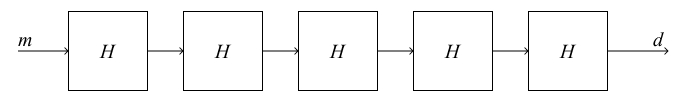
\includegraphics[width=1\textwidth]{Figures/background/hashchain_1.jpg}
  \caption[Hash chain]{}
  \label{fig:hash-chain-1}
\end{figure}

This concept was proposed by Lamport as a way to securely store passwords on servers~\cite{hashchain}. In his proposed protocol, the server just stores $H^n(p)$, where $p$ is the password and $n$ is relatively big number (for example, 1000). When the user wants to authenticate, she sends $H^{n-1}(p)$ and the server computes $H(H^{n-1}(p))$ and checks if it corresponds to $H^n(p)$. If this check succeeds, the user is authenticated and the server replace the stored value with $H^{n-1}(p)$. Next time she wants to authenticate again, she'll need to send $H^{n-2}(p)$ and this value will be checked against the previously sent digest $H^{n-1}(p)$. In this protocol, even if the transmission or the storage of the password is not secure, the user is safe.

Blockchain technology uses this idea to form the immutable chain of blocks: each block contains the hash of the previous one. Modifying a block would result in changing its hash, this would break the chain since all the following blocks would have to be recomputed, changing each digest. As shown in \ref{fig:hash-chain-2}, it's a slightly different concept than the plain hash chain, since on each step, the hashing is done on the previous digest linked to raw data of the current block, so $d_{n}=H(b_n~||~d_{n-1})$

\begin{figure}[H]
  \centering
  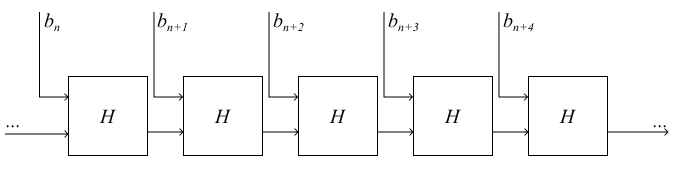
\includegraphics[width=1\textwidth]{Figures/background/hashchain_2.jpg}
  \caption[Hash chain in blockchain]{}
  \label{fig:hash-chain-2}
\end{figure}

\subsection{Merkle trees}

A Merkle tree is a data structure that generalizes the hash chain to efficiently prove membership of data. It's a binary tree in which each leaf node represents the hash of data, while intermediate nodes are computed as the hash of the two child nodes. Figure \ref{fig:merkle-tree} is an example of a Merkle tree with 4 leaf nodes.

\begin{figure}[H]
  \centering
  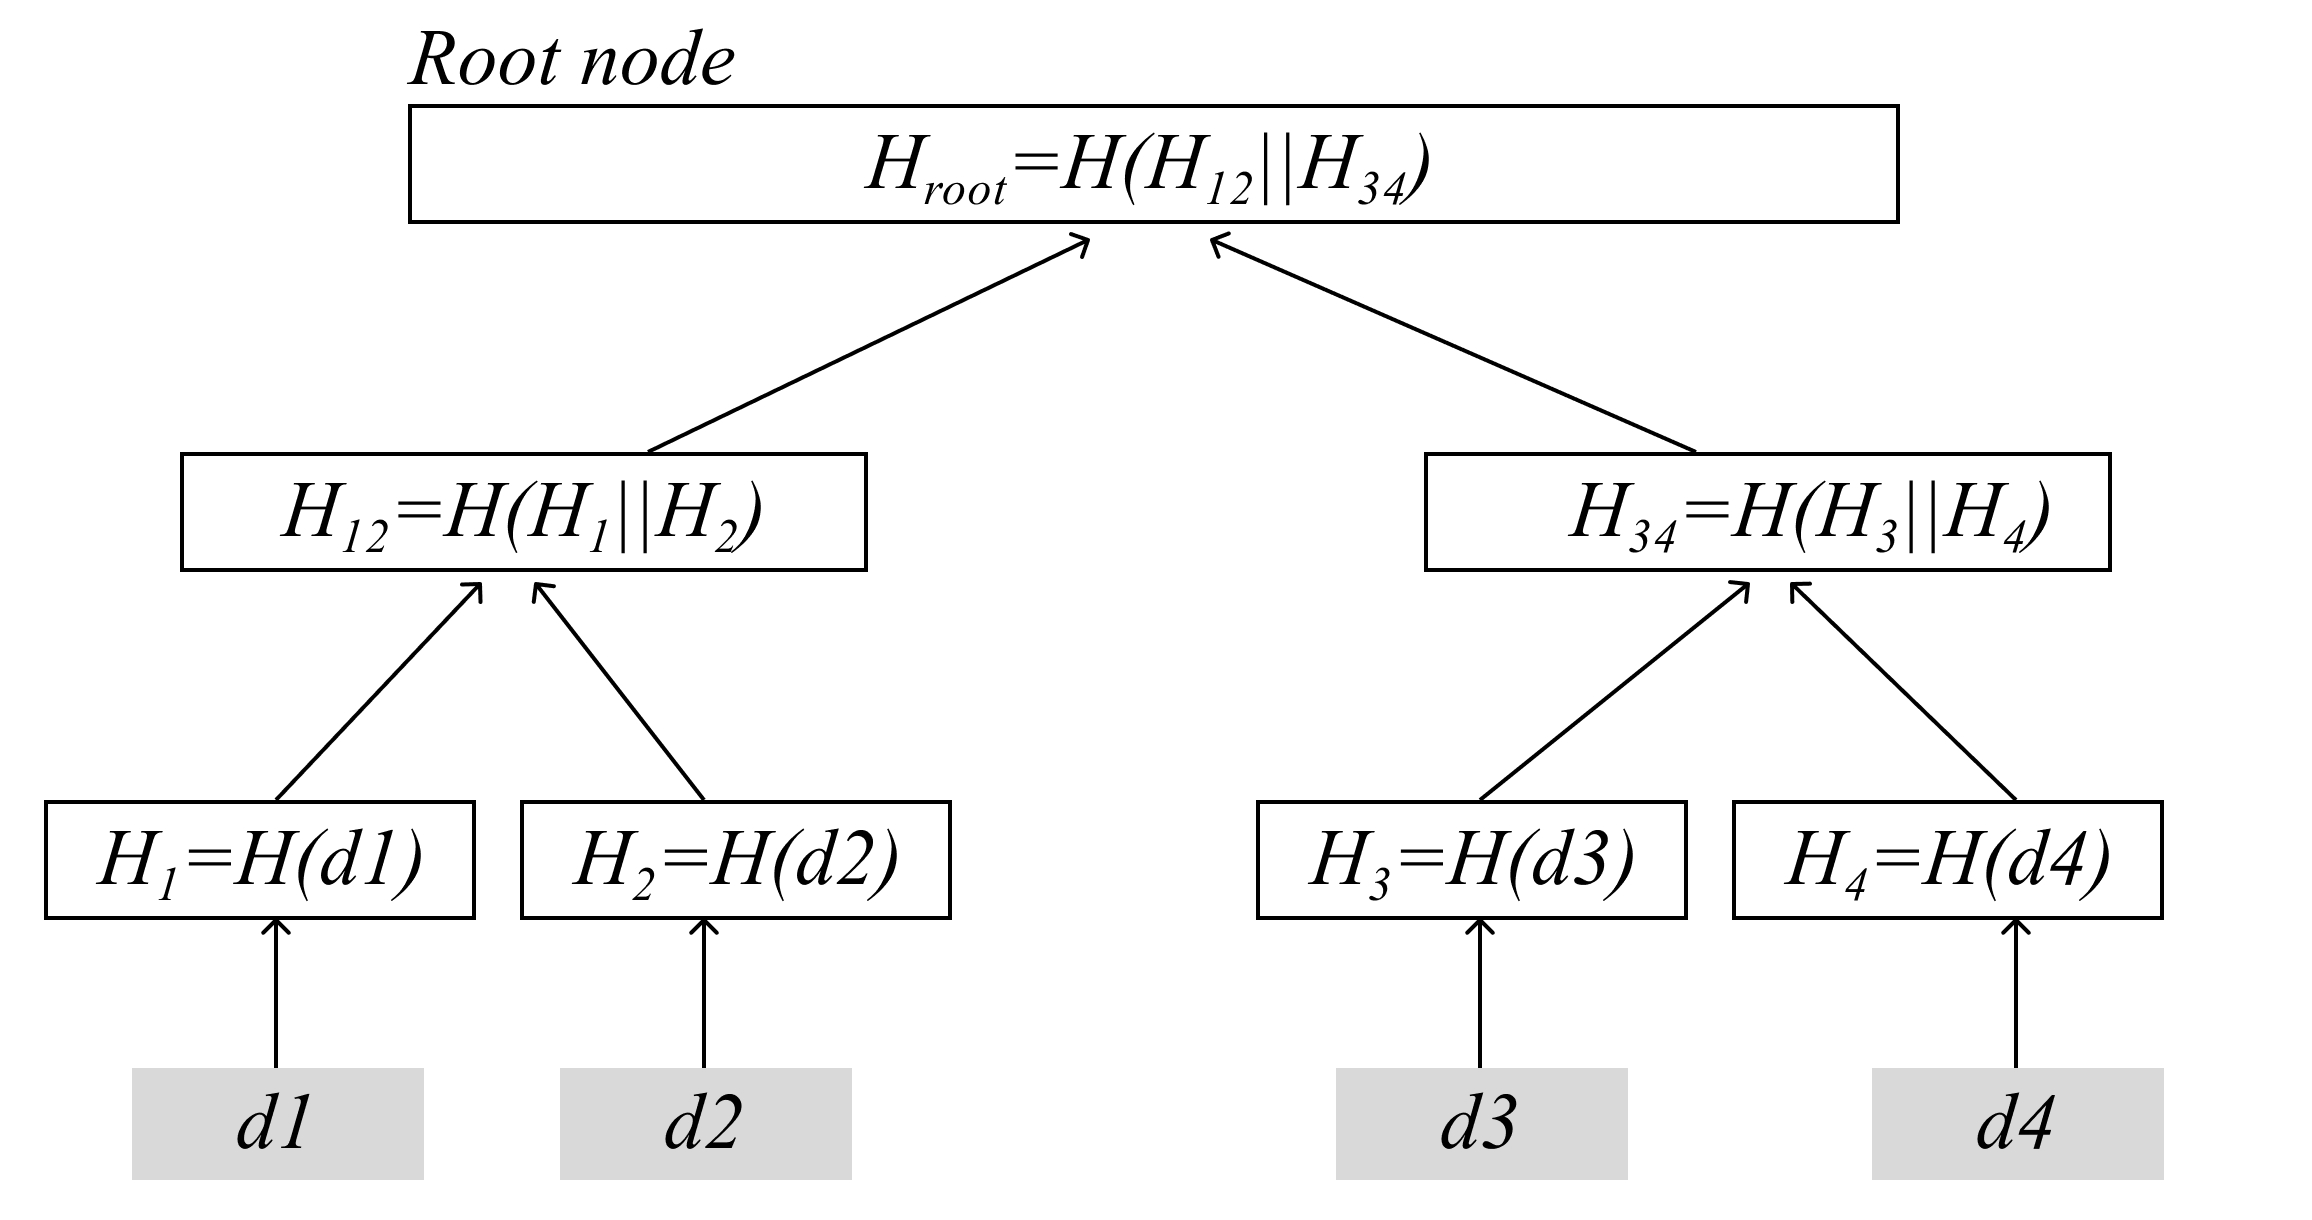
\includegraphics[width=1\textwidth]{Figures/background/merkle_tree.jpg}
  \caption[Merkle tree]{}
  \label{fig:merkle-tree}
\end{figure}

Proving membership of data to a tree with $2^n$ leaves just requires $n$ steps and $n$ intermediate nodes. The algorithm simply reconstructs the tree starting from the node that must be checked, recalculating again the root node. Data is proved to be part of the tree if the recalculated root node is equal to the given root node of the tree.

\subsection{Digital signatures}


\section{The blockchain}

What problem it's solving

\subsection{Double spending problem}

\subsection{Blockchain properties}

\subsection{Consensus layer}

\subsubsection{Proof of work}

\subsubsection{Proof of Stake}

\subsection{51\% attack}

\section{Ethereum}

\subsection{Ethereum as a state machine}

\subsection{Ethereum node}

\subsection{Smart Contracts}

\subsection{EVM}

\subsection{Solidity}

\subsection{ERC20 and ERC721}

% Eventually talk about Dgraph

% section{Graph databases}

% \subsection{Dgraph}




\cleardoublepage



\chapter{Previous work}

Data extraction and indexing from various blockchains is an essential topic for making Web3 and dApps working, there are different projects that have tried to address this problem. A lot of work has been done by companies, whose source code and methodology are not publicly available. There are also some open source or academic attempts that I will use as a comparison with my work. \\

\noindent These projects target three main categories:

\begin{itemize}
  \item Web3 and dApps developers, that need data to feed their applications.
  \item Data analysts, that need to analyse historical blockchain data. 
  \item Blockchain users, that need to see the results of transactions.
\end{itemize}

\noindent In the next sections I'll list the state of the art tools available.

\section{Etherscan}

Etherscan \footnote{https://etherscan.io/} is the reference point for accessing data about the Ethereum blockchain. It’s the most used explorer that lets people browse historical data trough a web interface. Here users can easily explore transactions, internal calls, token transfers and everything else related to the Ethereum protocol. It’s useful for inspecting singular operations, but it can’t be used for large scale analysis.

One of the most important service they offer is the verification of smart contracts, they host 461,261\footnote{This data was calculated using the CSV file exported from https://etherscan.io/chart/verified-contracts} source codes (as of 17 May 2023) that have been verified to match exactly the deployed bytecode on the  Ethereum chain. 

The process of verification consists in providing Etherscan the exact source code of a Smart Contract, the version of the compiler used, the license selected and the contract address to verify. With this information, Etherscan will try to compile the given data and check if the resulting bytecode equals the one deployed on the blockchain. There are plugins for the most used development tools like Remix or Hardhat that ease this process of verification.

This data is extremely helpful for understanding the semantic of the code deployed, since it's very hard to get useful insights by just looking at the raw bytecode. Many studies are based on these verified contracts.

Etherscan has evolved from being just an Ethereum explorer. They used the huge amount of data they have to create API endpoints and offer these data to users for a fee. These API endpoints include the standard Ethereum JSON-RPC interface and many more advanced methods, like tokens logic and specific indexes not supported by the standard RPC. 

On top of that, they also provide live and interactive charts\footnote{Available at https://etherscan.io/charts} about historical Ethereum data.

The same company that is behind the Ethereum Etherscan explorer applied the same logic and technology to other EVM compatible chains, like Polygon\footnote{https://polygonscan.com/} or BNB Smart Chain\footnote{https://bscscan.com/}.

It's important to note that, although they provide almost all the possible available Ethereum data, they haven't shared technical details about how this data is extracted or how it is indexed, users need to trust the company. Another problem is that using their data via the API for large scale analysis is unfeasible since it would be too expensive.


\section{The Graph}

The Graph~\cite{the-graph} is a decentralized indexing protocol for blockchain data. It allows users to get structured on-chain data from other users via a GraphQL\footnote{GraphQL is an open source query language created by Facebook.} interface. 

All the data is organized is so called \textbf{subgraphs} that are independent data collections that index a small subset of a blockchain network. A common pattern is that a subgraph indexes data from one or a set of few smart contracts all part of a common protocol, like Uniswap\footnote{\url{https://uniswap.org/}}. All the available subgraphs can be found on the explorer\footnote{https://thegraph.com/explorer}.

The underlying protocol is composed of multiple actors:

\begin{itemize}
  \item Developers: people with technical knowledge that develop the needed code for creating and maintaining the indexes. As of now, the most important pieces of code needed are the mappings from Ethereum events to the stored data (written in AssemblyScript\footnote{https://www.assemblyscript.org/}, a Typescript-like language that is compiled to WebAssembly) and the subgraph manifest, a structured description of all the parts needed by the subgraph in YAML format.  
  \item Indexers: they are responsible for operating a node, this implies indexing the data following a subgraph specification and serving queries.
  \item Curators: they are in charge of finding the best subgraphs to be indexed.
  \item Delegators: they secure the network by locking economical value to certain indexers they choose, giving them the possibility to serve more queries.
\end{itemize}

All these actors are economically motivated to perform well, this is achieved via a token economy where the GRT is the currency. It is implemented on the Ethereum chain with a standard ERC20 smart contract\footnote{https://etherscan.io/token/0xc944e90c64b2c07662a292be6244bdf05cda44a7}.

In order to index and serve queries, indexers have to stake at least 100,000 GRT tokens (roughly equal to 12K USD with the current change). These tokens can be slashed in case the indexer behaves maliciously. The more tokens the indexer stakes and the more queries it can serve. At the same time, indexers are rewarded with GRT tokens in two ways: query fees and annual rewards based on amount of queries served.

According to the specification of the subgraph file\footnote{https://github.com/graphprotocol/graph-node/blob/master/docs/subgraph-manifest.md\#15-data-source}, the only allowed source of data are Ethereum contracts and mappings are restricted to Events. Image \ref{fig:the-graph-data-flow} shows the flow of data in the protocol. In most cases, this is enough for dApps, since typically all the smart contracts are written in such a way that they emit events when things happen. 

On the other hand, it is not possible to index all the other kind of information for performing other analysis, such as block data, contract deployments, transactions, contracts destruction, etc. It is also not possible to extract data that was not meant to be extracted, since the emitted events are pieces of information that the developers of the smart contracts explicitly wanted to expose and index. 


\begin{figure}[H]
  \centering
  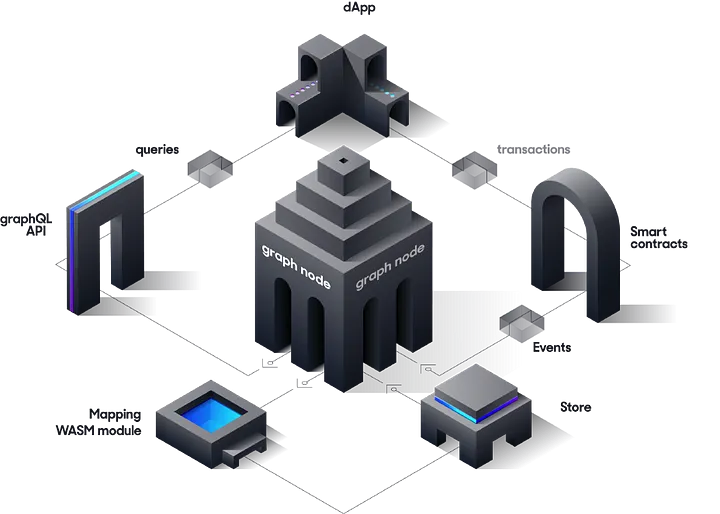
\includegraphics[width=1\textwidth]{Figures/graph-dataflow.png}
  \caption[The Graph data flow]{Data flow of The Graph indexing protocol\protect\footnotemark.}
  \label{fig:the-graph-data-flow}
\end{figure}

\footnotetext{Source: https://thegraph.com/docs/en/about/}


As of today, the protocol still relies on a central hosted service that uses the subgraphs logic and code to index data, but queries are served from this centralized server for free. This should change in 2023, the network should slowly migrate from this centralized service to the decentralized protocol once the quality of the service will be comparable \footnote{https://thegraph.academy/developers/sunsetting-the-hosted-service/}.

The Graph is the first attempt to decentralize indexing of blockchain data, it's still a project with a lot of work behind the scene. It's the most promising mechanism to make Web3 and dApps not dependant from centralized data ingestion services.


\section{Ethereum-ETL}

Ethereum-ETL\footnote{https://github.com/blockchain-etl/ethereum-etl} is an open source tool for extracting data from the Ethereum blockchain following the \textbf{Extract-Transform-Load} pattern. It's written in Python and can be used trough a CLI.

\noindent Raw data can be extracted to CSV or JSON files using these commands:

\begin{itemize}
    \item \verb|export_blocks_and_transactions|: it calls \verb|eth_getBlockByNumber| RPC and maps the response to two files containing blocks and transactions.
    \item \verb|export_token_transfers|: it calls \verb|eth_getFilterlogs| applying a filter with the first topic set to \verb|0xddf252...23b3ef|, the Keccak-256 hash of the ERC20 and ERC721 Transfer event signature. Transfers are stored in a single file without distinction between ERC20 or ERC721.   
    \item \verb|export_traces|: it stores the internal transactions calling the \verb|trace_block| method.
\end{itemize}

\noindent All other kind of data can be extracted starting from the files that these previous commands store. It is possible to further extract:

\begin{itemize}
    \item Transaction receipts and logs starting from transaction hashes exported from \verb|export_blocks_and_transactions|.
    \item Contracts data, starting from the traces stored with \verb|export_traces|.
    \item Token contracts with metadata, starting from contracts (this requires two previous step of extraction). 
\end{itemize}

\subsection{Google BigQuery public dataset}

\noindent Ethereum-ETL also allows for streaming these data from an Ethereum node to the console. This functionality is used to ingest data into the popular Ethereum Google BigQuery public dataset\footnote{https://cloud.google.com/blog/products/data-analytics/ethereum-bigquery-public-dataset-smart-contract-analytics}. This dataset is organized in six tables that I'll report here since it's a good representation of the raw data that can be extracted from an Ethereum node.

\begin{table}[H]
\centering
    \begin{tabular}  { m{6cm} m{3cm} m{3cm} } 
    \toprule
    \textbf{Attribute} & \textbf{Type} & \textbf{Required} \\
    \midrule
    timestamp & Timestamp & Yes\\ %& The timestamp for when the block was collated	\\
    number & Integer & Yes\\ %& & The block number \\
    hash & String & Yes\\ %& & Hash of the block \\
    parent\_hash & String & No\\ %& & Hash of the parent block\\
    nonce & String & Yes\\ %& Hash of the generated proof-of-work \\
    sha3\_uncles & String & No\\ %& & SHA3 of the uncles data in the block \\
    logs\_bloom & String & No\\ %& & The bloom filter for the logs of the block \\
    transaction\_root & String & No\\ %& & The root of the transaction trie of the block \\
    state\_root& String & No\\ %& & The root of the final state trie of the block \\
    receipt\_root & String & No\\ %& & The root of the receipts trie of the block \\
    miner & String & No\\ %& & The address of the beneficiary to whom the mining rewards were given \\
    difficulty & Numeric & No\\ %& & Integer of the difficulty for this block\\
    total\_difficulty & Numeric & No\\ %& & Integer of the total difficulty of the chain until this block\\
    size & Integer & No\\ %& & The size of this block in bytes\\
    extra\_data & String & No\\ %& & The extra data field of this block\\
    gas\_limit & Integer & No\\ %& & The maximum gas allowed in this block\\
    gas\_used & Integer & No\\ %& & The total used gas by all transactions in this block \\
    transaction\_count & Integer & No\\ %& & The number of transactions in the block \\
    base\_fee\_per\_gas & Integer & No\\ %& & Protocol base fee per gas, which can move up or down \\
    withdrawals\_root & String & No\\ %& & The root of the withdrawal trie of the block\\
    withdrawals & Record & Repeated\\ %& & Validator withdrawals \\
    \quad- index & \quad- Integer & \quad- No\\ %& &  \\
    \quad- validator\_index & \quad- Integer & \quad- No\\ %& & \\
    \quad- address & \quad- Integer & \quad- No\\ %& & \\
    \quad- amount & \quad- Integer & \quad- No\\ %& & \\
    \bottomrule
\end{tabular}
\caption[Google BigQuery \texttt{Blocks} table]{Description of table Blocks on the Google BigQuery public dataset, from the official docs.}
\label{table:bigquery-blocks}
\end{table}

\begin{table}[H]
\centering
    \begin{tabular}  { m{6cm} m{3cm} m{3cm} } 
    \toprule
    \textbf{Attribute} & \textbf{Type} & \textbf{Required} \\
    \midrule
    log\_index & Integer	& Yes \\
    transaction\_hash & String & Yes \\
    transaction\_index & Integer & Yes	\\		
    address & String & No \\
    data & String & No \\
    topics & String & Repeated \\
    block\_timestamp & Timestamp & Yes \\ 
    block\_number & Integer & Yes \\
    block\_hash & String & Yes \\
    \bottomrule
\end{tabular}
\caption[Google BigQuery \texttt{Logs} table]{Description of table Logs on the Google BigQuery public dataset, from the official docs.}
\label{table:bigquery-logs}
\end{table}

\begin{table}[H]
\centering
    \begin{tabular}  { m{6cm} m{3cm} m{3cm} } 
    \toprule
    \textbf{Attribute} & \textbf{Type} & \textbf{Required} \\
    \midrule
    address & String & Yes \\
    bytecode & String & No \\
    function\_signature & String & repeated \\
    is\_erc20 & Boolean & No \\
    is\_erc721 & Boolean & No \\
    block\_timestamp & Timestamp & Yes \\
    block\_number & Integer & Yes \\
    block\_hash & String & Yes \\
    \bottomrule
\end{tabular}
\caption[Google BigQuery \texttt{Contracts} table]{Description of table Contracts on the Google BigQuery public dataset, from the official docs.}
\label{table:bigquery-contracts}
\end{table}

\begin{table}[H]
\centering
    \begin{tabular}  { m{6cm} m{3cm} m{3cm} } 
    \toprule
    \textbf{Attribute} & \textbf{Type} & \textbf{Required} \\
    \midrule
    transaction\_hash & String &	No	\\			
    transaction\_index & Integer	& No	\\			
    from\_address & String &	No \\	
    to\_address & String & No \\				
    value & Numeric &	No		\\		
    input & String &	No		\\		
    output & String	& No		\\		
    trace\_type & String &	Yes		\\		
    call\_type & String	& No	\\
    reward\_type & String	& No\\
    gas & Integer	& No\\
    gas\_used & Integer	& No\\
    subtraces & Integer	& No\\
    trace\_address & String	& No		\\
    error & String	& No		\\
    status & Integer	& No	\\		
    block\_timestamp & Timestamp	& Yes		\\		
    block\_number & Integer	& Yes			\\	
    block\_hash & String	& Yes	\\			
    trace\_id & String	& No \\
    \bottomrule
\end{tabular}
\caption[Google BigQuery \texttt{Traces} table]{Description of table Traces on the Google BigQuery public dataset, from the official docs.}
\label{table:bigquery-traces}
\end{table}

\begin{table}[H]
\centering
    \begin{tabular}  { m{6cm} m{3cm} m{3cm} } 
    \toprule
    \textbf{Attribute} & \textbf{Type} & \textbf{Required} \\
    \midrule
    token\_address & String & Yes	 \\			
    from\_address & String & No \\
    to\_address & String	& No	\\			
    value & String	& No	\\
    \bottomrule
\end{tabular}
\caption[Google BigQuery \texttt{Token\_transfers} table]{Description of table Token\_transfers on the Google BigQuery public dataset, from the official docs.}
\label{table:bigquery-transfers}
\end{table}

\begin{table}[H]
\centering
    \begin{tabular}  { m{6cm} m{3cm} m{3cm} } 
    \toprule
    \textbf{Attribute} & \textbf{Type} & \textbf{Required} \\
    \midrule
    hash & String	& Yes		\\		
    nonce & Integer	& Yes \\				
    transaction\_index & Integer	& Yes		\\		
    from\_address & String	& Yes			\\	
    to\_address & String	& No		\\		
    value & Numeric	& No \\				
    gas &  Integer	& No \\				 
    gas\_price &  Integer &	No \\				
    input &  String	& No \\				
    receipt\_cumulative\_gas\_used & Integer & 	No \\				
    receipt\_gas\_used  & Integer	& No \\				
    receipt\_contract\_address & String	& No \\				
    receipt\_root &  String & 	No \\				
    receipt\_status  & Integer & 	No \\				
    block\_timestamp  & Timestamp	 & Yes \\				
    block\_number  & Integer & 	Yes \\				
    block\_hash & String &	Yes \\				
    max\_fee\_per\_gas & Integer	& No \\	
    max\_priority\_fee\_per\_gas & Integer	& No \\		
    transaction\_type & Integer	& No				\\
    receipt\_effective\_gas\_price & Integer	& No	\\
    \bottomrule
\end{tabular}
\caption[Google BigQuery \texttt{Transactions} table]{Description of table Transactions on the Google BigQuery public dataset, from the official docs.}
\label{table:bigquery-transactions}
\end{table}

It is possible to query these tables using SQL syntax, they can be joined on equal fields. There is the possibility to query this database for free up to a certain monthly limit of processing storage and amount of data extracted. 

I'll compare Ethereum-ETL with my work in the next chapters.

\section{Dune analytics}

Dune Analytics\footnote{https://dune.com/home} is a company that provides tools to query and visualize data from multiple blockchains. They support Bitcoin, Solana, Ethereum and other 8 EVM chains.\\

Their application is web-based, from there it is possible to create queries using SQL syntax and visualize results in interactive charts. Multiple queries can be collected together to create dashboards\footnote{Example of a dashboard about history of Ethereum: https://dune.com/hildobby/ethereum}.  

\subsection{Data architecture}

Blockchain data was initially managed using PostgreSQL and SparkSQL until 2022, year in which they released their own engine called DuneSQL \footnote{https://dune.com/blog/dune-engine-v2}, migration to this technology is currently ongoing. \\

They started storing and indexing data with PostgreSQL.
In this DBMS entries are stored in pages following a row-oriented strategy, which means that all the attributes of a row are stored adjacently. This is beneficial when it's necessary to retrieve all the attributes of a row while querying. However, it leads to poor performance when filtering for specific attributes, since the database has to load many bytes containing irrelevant data (i.e., all the other attributes of the row that are not used). To optimize this, it is possible to create indexes on columns. These indexes will provide very good performance, but can be hard and slow to maintain, specially with huge amount of data. At Dune Analytics they tried this approach with traditional relational database combined with indexes, but they had to drop it stating that "the size of the datasets were so huge that the database was struggling to fully support them"\footnote{Source: https://dune.com/blog/introducing-dune-sql}. \\

So they came up with DuneSQL, a query engine built specifically for managing blockchain data. It's a fork of Trino, an open source distributed SQL query engine designed to query data from heterogeneous sources. The DuneSQL fork is not open source, so technical information can only be deducted from their blog articles or statements on the support community. The main features they added are \textit{varbinary} data type for storing addresses and hashes, as well as \textit{uint256} support for EVM data. \\

Data is physically stored on AWS S3 buckets using the Apache Parquet storage format\footnote{https://github.com/apache/parquet-format}. This storage system is a mix between column and row oriented. Data is split in files based on rows, inside these files, there are further row groups and inside these groups data is divided by columns. Image \ref{fig:parquet-structure} visualize this concept. \\

\begin{figure}[H]
  \centering
  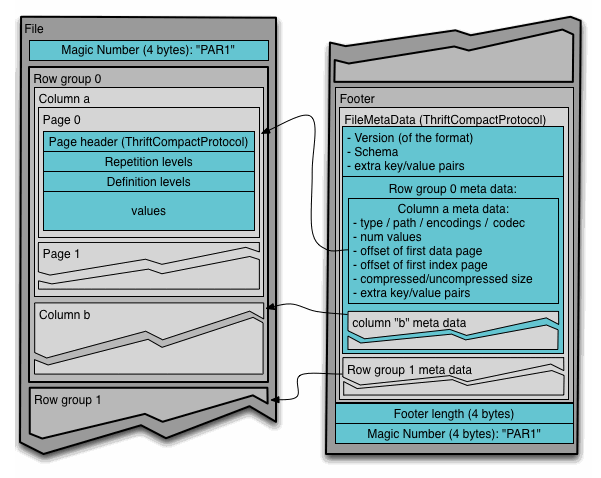
\includegraphics[width=1\textwidth]{Figures/parquet-structure.png}
  \caption[Parquet storage format structure]{File structure in the Parquet storage format\protect\footnotemark.}
  \label{fig:parquet-structure}
\end{figure}

\footnotetext{Source: https://github.com/apache/parquet-format}

Indexing is done using the Parquet file's metadata. At the end of each file there's a part in which are stored min/max values of all the column values inside a page, as shown in image \ref{fig:parquet-index}. This information allows the database to skip reading the whole chunk if values are not in the desired range. While working great for certain types of data, it isn't very useful with strings, especially if they are not sorted. That's the reason why even a simple query like \ref{lst:dune-query} can take several minutes to run. \\

\begin{figure}[H]
  \centering
  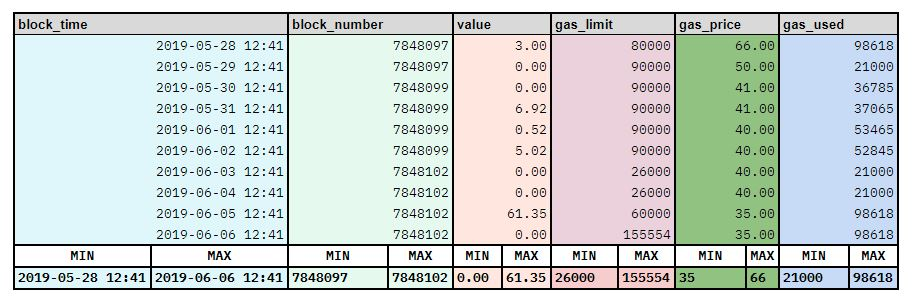
\includegraphics[width=1\textwidth]{Figures/parquet-index.jpg}
  \caption[Parquet ColumnIndex on Dune Analytics]{Parquet min/max column index structure \protect\footnotemark. }
  \label{fig:parquet-index}
\end{figure}

\footnotetext{Source: https://dune.com/docs/query/storage/}

\begin{lstlisting}[language=SQL,caption={Shortened simple query on DuneSQL that took 3 minutes to run},label={lst:dune-query},captionpos=b]
Select * from ethereum.transactions
where hash = 0x9ef65fe51...ff74219e
\end{lstlisting}

\subsection{Available data}

On Dune Analytics, blockchain data is available in multiple layers:

\begin{itemize}
    \item \textit{Raw tables}: these tables contain raw data as it is stored on the various blockchains, without modifications. For EVM chains this means Blocks, Logs, Traces and Transactions.
    \item \textit{Decoded tables}: verified contracts receive their own tables on which data is stored in a more readable way. Each event and function that is present in the contract's ABI corresponds to a table on Dune with the following name pattern: \texttt{project\_chain.contract\_[evt/call]\_evtOrCallName}. Inside this table there will be columns for each of the event or function attributes, with the relative names. For example, all the \textit{cryptokitties} \texttt{Transfer} events are stored in a table called \texttt{cryptokitties\_ethereum.KittyCore\_evt\_Transfer} that will have, among other contextual information, three columns: \textit{from}/\textit{to} addresses and \textit{tokenId}.
    \item \textit{Spellbooks}: these tables are abstractions over raw and decoded data that give users an easy way to retrieve information without diving into the technicalities of complex decentralized protocols. They're open source and the community can contribute creating new spellbooks on the Github Repository\footnote{https://github.com/duneanalytics/spellbook}. The main power of spellbooks is to put together data from heterogeneous sources to gather useful insights. The most clear example is the \texttt{dex.trades}\footnote{https://github.com/duneanalytics/spellbook/blob/main/models/dex/dex\_trades.sql} spellbook, that puts together all the trades made on all decentralized exchanges of all the blockchains present on Dune Analytics.
\end{itemize}

\section{XBlock-ETH}

Zheng et al.~\cite{xblock-eth} released a dataset containing raw Ethereum data and described the framework used for getting it, called XBlock-ETH. It was released in 2019 and data is periodically updated in chunks of 500,000 blocks, currently it covers blocks from 0 to 16,499,999. It is divided in different smaller datasets: \textit{Block}, \textit{Block Transaction}, \textit{Internal Transaction}, \textit{Contract Info}, \textit{ERC20 Transaction}, \textit{ERC721 Transaction}, \textit{Token Info}. Data can be downloaded from their website\footnote{https://xblock.pro/xblock-eth.html} in CSV format.

This is a useful resource for getting Ethereum data without having the possibility to run a node; however it lacks important information such as logs and receipts. 

It's not easy to use, since the massive amount of data in the CSV files must be parsed and cannot be easily queried or indexed, further transformation steps are needed. There are some Python scripts available on Github\footnote{https://github.com/tczpl/XBlock-ETH} for downloading and analysing the data, but the code used for the extraction is not open source, so it's not possible to know exactly how information was retrieved.

\section{Data-ether}

DateEther \cite{dataether} is a framework presented by Chen et al. for extracting and indexing Ethereum data. They tried a different approach for executing this task: they modified a Geth\footnote{https://geth.ethereum.org/} node to record and store data during the initial synchronization phase. They used ElasticSearch\footnote{https://www.elastic.co/} for indexing and exploring data, but by the time of their research the size of data was relatively small compared to now.

While extracting data by modifying a node source code was efficient back in 2019, now Ethereum nodes have evolved and there are different and faster RPCs for getting internal transactions. Their way of extracting data was compared against \texttt{debug\_traceTransaction} RPC of Geth, claiming to be 18.6x faster, but it wasn't compare against \texttt{debug\_traceBlock} or \texttt{trace\_block} of Erigon\footnote{https://github.com/ledgerwatch/erigon}. From my work, using Erigon's \texttt{trace\_block} RPC, I managed to get and loop trough all the internal transactions in around 9 hours (40 including transactions and logs). Doing that while synchronizing a node would have required at least 3-4 days. 

Extracting data by modifying source code has another drawback: maintainability. Just Geth itself received 173 releases\footnote{https://github.com/ethereum/go-ethereum/releases}, modifying its source code would mean having to merge the code and resolving eventual conflicts every time a new release is published. This is not a problem using Ethereum RPC APIs since they don't change after upgrades of the nodes.

\section{Web3 providers}

The term "Web3 provider" is commonly used to refer to companies that offer access to Ethereum RPC API, avoiding developers of Web3 dApps the costs of running a node. They're included in this chapter since the majority of them also provide access to indexed and interpreted data. Some popular web3 providers include Alchemy\footnote{https://www.alchemy.com/}, Infura\footnote{https://www.infura.io/}, Quicknode\footnote{https://www.quicknode.com/} and Chainstack\footnote{https://chainstack.com/}.

All of them have endpoints for getting NFTs data, it's possible to get all NFTs owned by an address by just calling an API instead of having to analyze all the chain. Chainstack also hosts on their servers all the supgraphs of "The Graph" protocol, offering users the possibility to use a more stable service instead of the decentralized alterntive.

It is important to note that the web3 providers are profit-oriented companies. While they provide an important service in the world of dApps, it's essential to consider their cost implications. Using their services for analyzing historical data can be very expensive, since billing is done based on number of API requests to their server.

Another important aspect to consider is the transparency of these services. As profit-oriented entities, these web3 providers do not necessarily make their source code and methodology open source. This means that developers relying on their services need to trust the data they receive. 

Depending on centralized companies poses also a risk to the actual decentralization of the web3. Access to the blockchain infrastructure is concentrated on a few companies, as noted by Wang et al.~\cite{wang2022exploring}.

\section{Comparison}

I summarized in table \ref{table:tools-comparison} the main differences between the tools in terms of \textit{primary target}, \textit{transparency} and \textit{price}.

\begin{table}[ht!]
\centering
    \begin{threeparttable}
    \begin{tabular}  { m{3cm} m{3cm} m{1.5cm} m{5cm} } 
    \toprule
    \textbf{Tool} & \textbf{Target} & \textbf{Open source} & \textbf{Price}  \\
    \midrule
    Etherscan    & Blockchain users  & No & Free explorer, paid apis  \\[2.3ex]
    The Graph     & Web3 developers & Yes & Billing based on usage  \\[1.3ex]
    Ethereum-ETL     & Data analysts & Yes & Free  \\[1.3ex]
    Dune Analytics      & Data analysts & No & Based on query credits, it has free plan \\[2.6ex]
    XBlock-ETH  & Data analysts & No\tnote{*} & Free   \\[1.3ex]
    DataEther  & Data analysts & No\tnote{*} & Free   \\[1.3ex]
    Web3 providers      & Web3 developers & No & Billing on usage, they have free plans   \\[1.6ex]
    \bottomrule
    \end{tabular}
    \begin{tablenotes}
      \item[*] Source code not available, but they released technical papers describing the software.
      \end{tablenotes}
    \end{threeparttable}
\caption[State of the art tools comparison]{Comparison of state-of-the art tools for management of blockchain data.}
\label{table:tools-comparison}
\end{table}

\cleardoublepage



\chapter{Methods}

\noindent In this chapter, I introduce {\tt eth2dgraph}, the new open-source software designed to facilitate the extraction and indexing of Ethereum data in Dgraph.

Eth2dgraph is developed using Rust, a system programming language that prioritizes both speed and safety. Rust was chosen mainly for two reasons. Firstly, for its emphasis on performance and parallelism, crucial for scaling the data extraction process and achieving good performance. Secondly, Rust benefits from a rich ecosystem of libraries specifically designed for handling Ethereum data, easing the process of development.

One of the key features of eth2dgraph is its integration with a decompiler, enabling the extraction at scale of the Application Binary Interface (ABI) from the bytecode stored on the Ethereum blockchain. 

The following sections provide details about the architecture of eth2dgraph, give a comprehensive overview of how the software operates, and how it has been constructed.

\section{Data flow}

Extracting and indexing Ethereum Smart Contract data is a process of moving and transforming bytes. Raw data stored in the Ethereum node must be taken, transformed and ingested into a database, Dgraph in this case, in order to be indexed. 

The first attempt was to do this step through transactions. I ran a Dgraph cluster and instructed eth2dgraph to add data via DQL mutations. DQL stands for \textbf{Dgraph Query Language} and it is the language used to write Dgraph queries. This data flow was working but it was too slow for thinking about applying it to all the history of the Ethereum chain. I also had problems to parallelize data insertion, too many concurrent transactions were failing due to read-write conflicts. \cref{fig:data-flow-1} visualizes this data flow.

\begin{figure}[H]
\centering
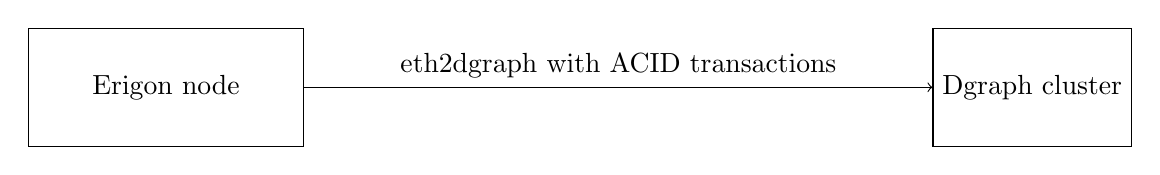
\begin{tikzpicture}
    \node[draw,minimum width=35mm,minimum height=15mm] (erigon) at (0,0) {Erigon node};
    \node[draw, minimum width=25mm,minimum height=15mm] (dgraph) at (11,0) {Dgraph cluster};
    \draw[->] (erigon) edge node[sloped, above] {eth2dgraph with ACID transactions} (dgraph);
\end{tikzpicture}
\caption[First attempt of data ingestion into Dgraph]{First attempt of data ingestion into Dgraph}
\label{fig:data-flow-1}
\end{figure}

To solve these problems, I changed the approach and followed an ETL (Extract, Transform, Load) process. Extraction and transformation are done in the same step by eth2dgraph. The output is stored in JSON files that can be later loaded into Dgraph using the Bulk Loader.

The Bulk Loader\footnote{Detailed description of the Bulk Loader: \url{https://dgraph.io/blog/post/bulkloader/}} is a tool provided by Dgraph. It is designed for performing the initial load of data into the database. It takes JSON or RDF N-Quads\footnote{N-Quads is a serialization format for RDF graphs data \url{https://www.w3.org/TR/n-quads/}.} data and stores it directly in Badger, the underlying key-value database used by Dgraph. This is the fastest way to ingest data into Dgraph. It maximizes concurrency and avoid problems related to ACID constraints since it is not operating on a live database. \cref{fig:data-flow-2} visualizes the final data flow chosen for eth2dgraph.

\begin{figure}[H]
\centering
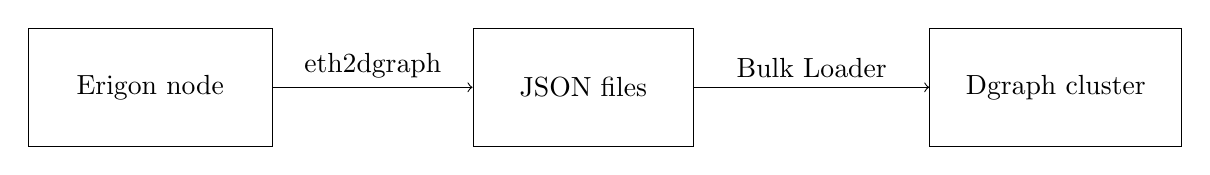
\begin{tikzpicture}
    \node[draw,minimum width=31mm,minimum height=15mm] (erigon) at (0,0) {Erigon node};
    \node[draw, minimum width=28mm,minimum height=15mm] (json) at (5.5,0) {JSON files};
    \node[draw, minimum width=32mm,minimum height=15mm] (dgraph) at (11.5,0) {Dgraph cluster};
    \draw[->] (erigon) edge node[sloped, above] {eth2dgraph} (json);
    \draw[->] (json) edge node[sloped, above] {Bulk Loader} (dgraph);
\end{tikzpicture}
\caption[Second and final data flow]{Second and final data flow}
  \label{fig:data-flow-2}
\end{figure}

\section{Data model}

After seeing how data is indexed in other works, I decided to design the schema in a slightly different way. In eth2dgraph, raw data is interpreted to create a schema around the semantics that can be extracted from the blockchain. This semantics is indexed alongside the raw Ethereum data. \cref{fig:schema} shows the whole schema that was created. All the edges have the {\tt @reverse} index, that means they can be traversed in both directions. Some of the attributes are indexed at load time, but it is easy to add indexes once the database is running. The complete description of both DQL and GraphQL schemas are described in~\cref{app-b}.

% TODO: update schema with final version

\begin{figure}[H]
  \centering
  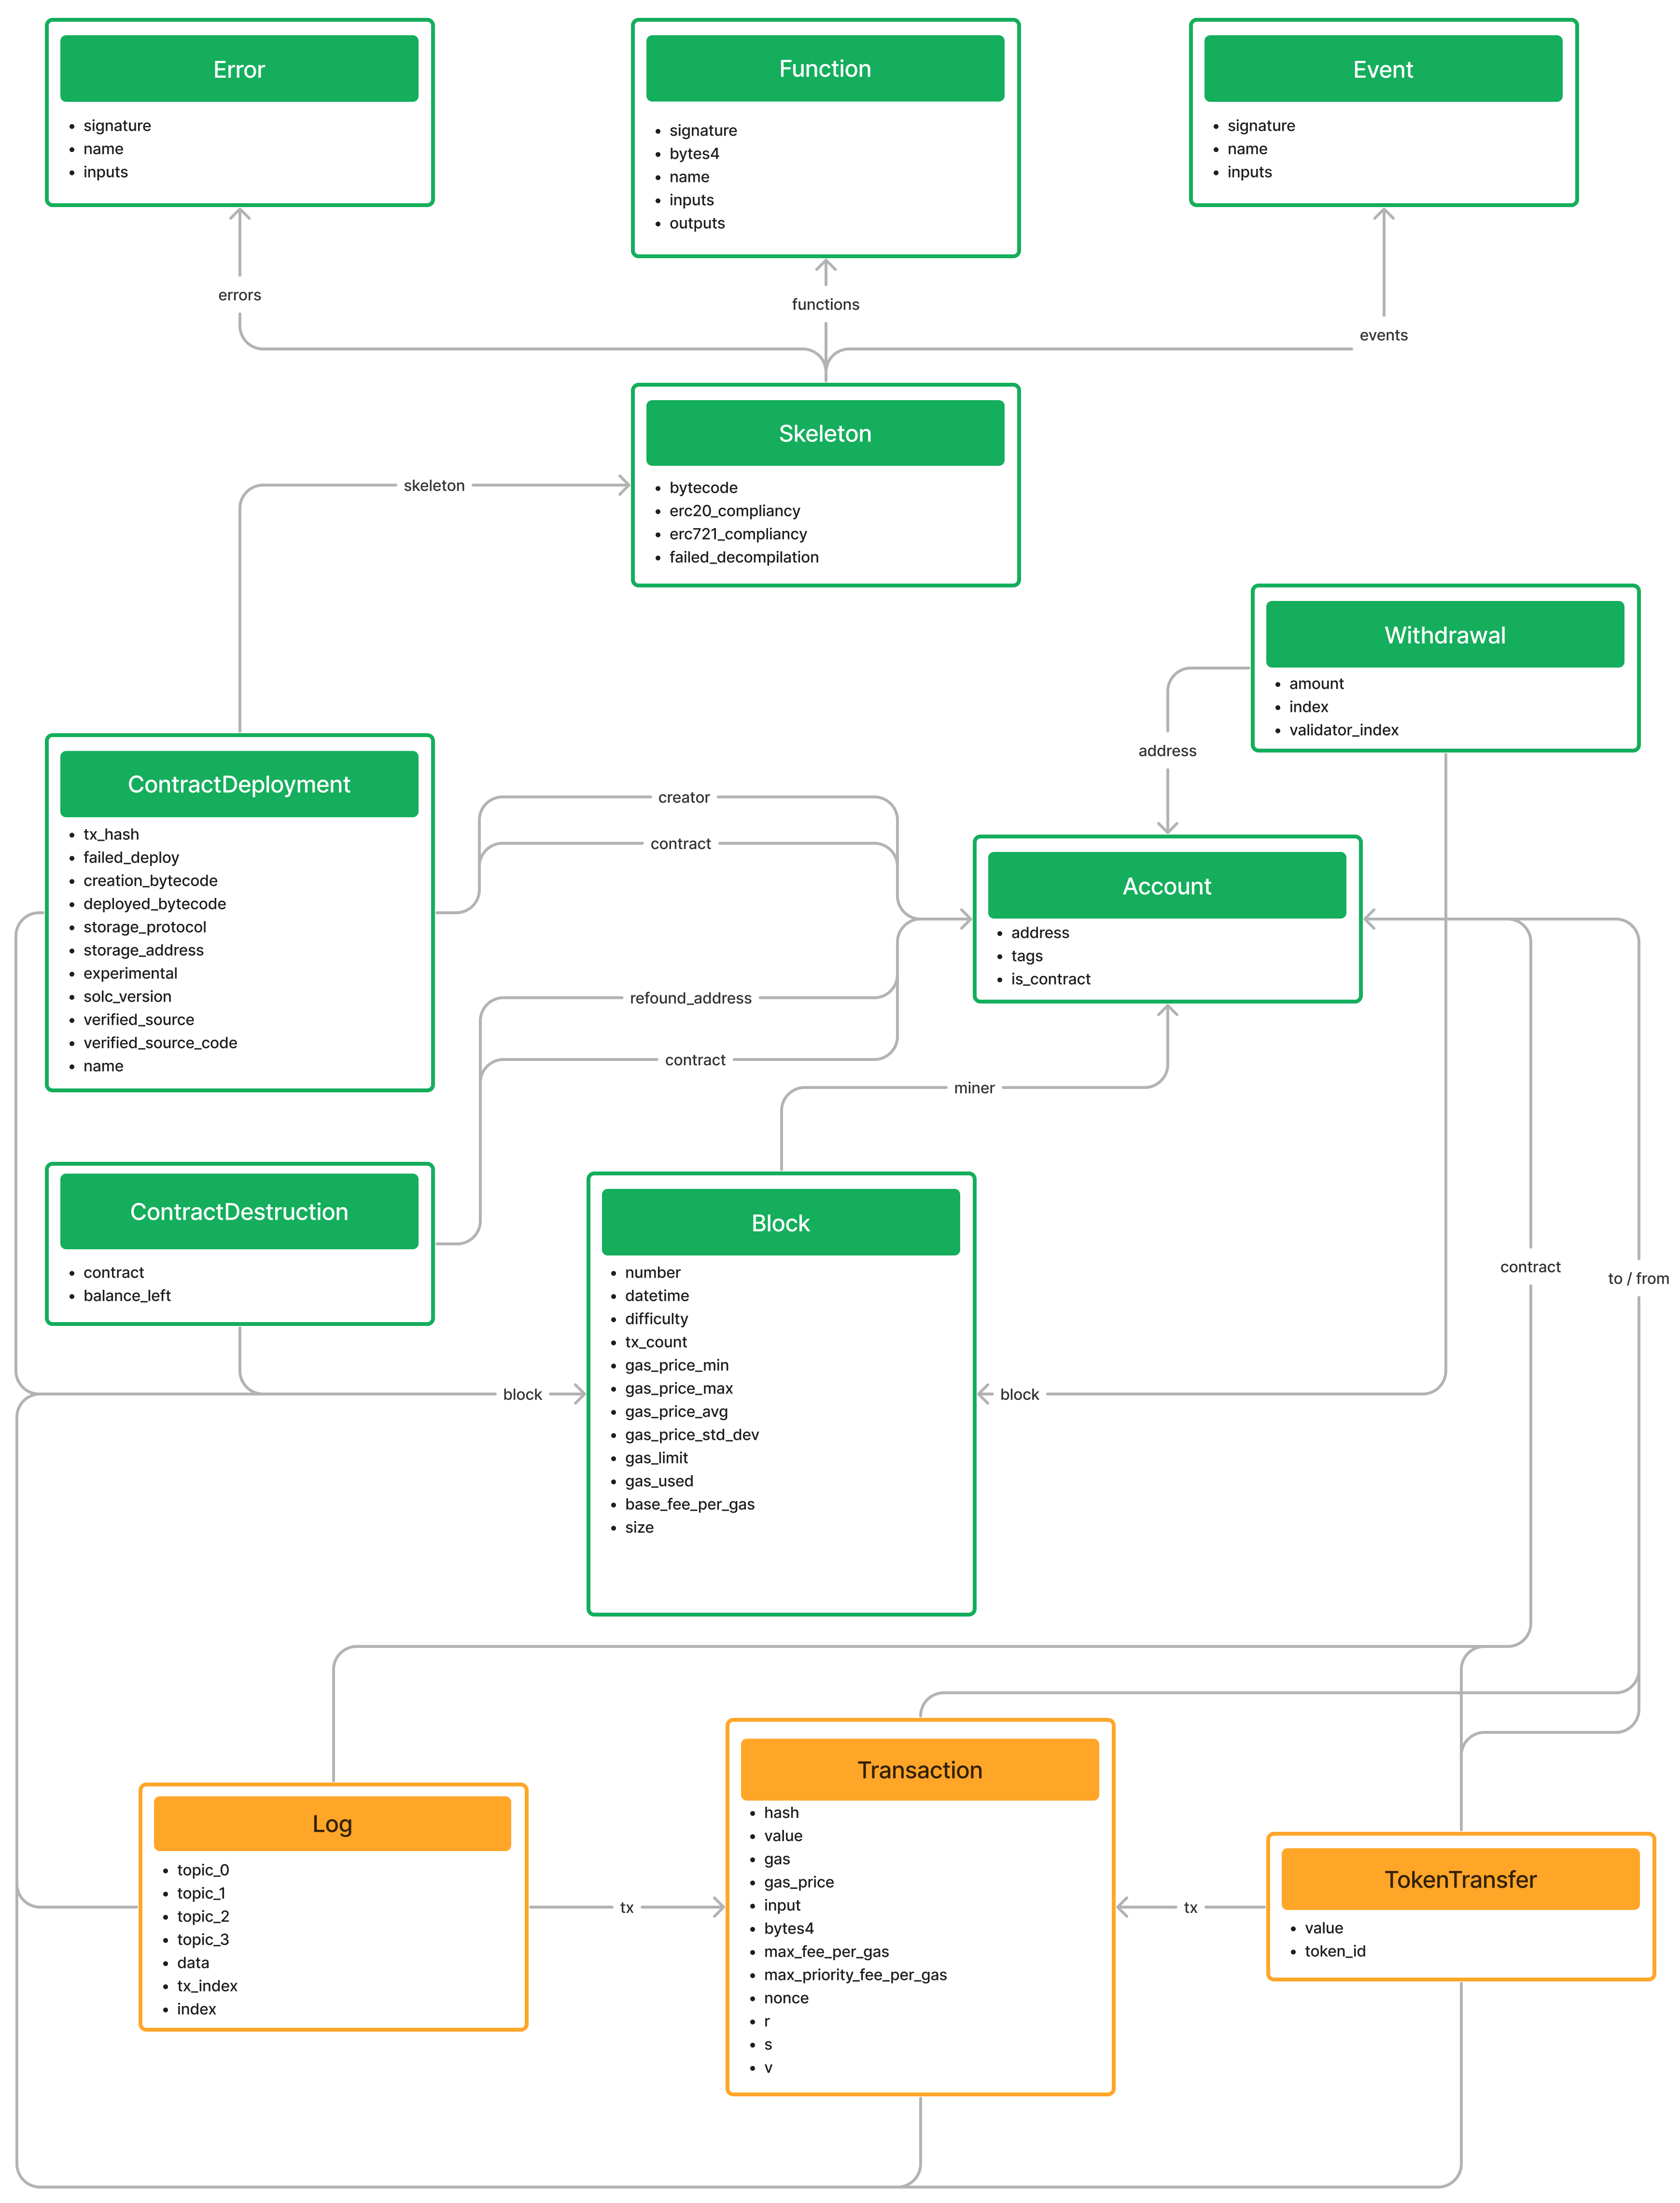
\includegraphics[width=1\textwidth]{Figures/methods/schema.png}
  \caption[Schema of Ethereum indexed data in Dgraph]{Schema of Ethereum indexed data in Dgraph}
  \label{fig:schema}
\end{figure}

Data is modeled as a graph with many edges. This was done since Dgraph is designed and optimized to perform joins and traversals.

Entities in yellow (\textit{Transaction}, \textit{TokenTransfer} and \textit{Log}), also called \textit{dynamic}, are optional and can be skipped during data extraction. Excluding data about smart contracts usage allows the creation of a much smaller dataset that provides a static description of these contracts. The reason of this choice is that the volume of dynamic data is around 30-40x bigger than static data. Having the option to extract a smaller dataset enables analysis on less powerful computers, improving the accessibility of the research. \\

\noindent Here is a brief description of the schema:

\begin{itemize}

    \item \textit{Transaction} and \textit{Log} are stored as they are retrieved from the Ethereum node. References to other entities are stored as edges for allowing graph traversal in queries. A \textit{Transaction} represents a transfer of value between two EOAs or an invocation of a Smart Contract from an EOA. A \textit{Log} is the result of an invocation of an Event in the code of a Smart Contract.

    \item \textit{TokenTransfer} represents both an ERC20 or an ERC721 token transfer between two accounts. Value is stored as a string since Dgraph does not handle 256 bit integers.
    
    \item \textit{Block} contains all the information related to a single Ethereum block. It includes data related to the withdrawals of validators. This entity is connected to many others: \textit{ContractDeployment}, \textit{ContractDestruction}, \textit{Transaction}, \textit{TokenTransfer} and \textit{Log}. 
    
    The indexed attribute \textit{datetime} is the only reference to time in the database, so it is possible to query it for specific dates and times and then get all the connected data from there. 

    \item \textit{Account} represents an Externally Owned Account or a Contract Account. Its fundamental attribute is the \textit{Address} of the account. There is also a boolean field \textit{is\_contract} indicating whether the account is a contract or not. This entity is extremely useful for querying data, since with the standard Ethereum RPC interface it is not possible to query data based on account addresses. So, for example, it is impossible to get all the transactions from/to an address without having to download and filter all the transactions in the history of Ethereum.

    \item \textit{ContractDeployment} and \textit{ContractDestruction} represent respectively the birth and the death of the code of a Smart Contract. I decided to store them in this way since I found, analyzing the data, that a single Ethereum Address can receive more than one code deployment, contrary to what it may appear because of the theoretical immutability of Smart Contracts. An address can receive both a deployment with the same old code or with new different code, in which case it is called \textit{morphic} or \textit{metamorphic}~\cite{create2-metamorphic}.

    \item I introduced the concept of \textit{Skeleton} directly in the schema since it is a useful way of aggregating similar contracts together. A \textit{Skeleton} is the bytecode of a contract without all the arguments of the PUSH opcodes. Having it directly in the schema allows to easily find contracts sharing the same skeleton.

    \item \textit{Event}, \textit{Function} and \textit{Error} are the parts that, together, form the ABI of the contracts. There is just one entity for each signature, so all the contracts implementing the same function/event/error point to the same entity. Having them indexed in this way allows to search contracts based on the functionalities they implement.
    
\end{itemize}

\section{Data extraction}

Data is extracted using the Ethereum \textit{Remote Procedure Call} (RPC) interface\footnote{Official specification of the Ethereum RPC interface: \url{https://ethereum.github.io/execution-apis/api-documentation/}}. Eth2dgraph extracts data block by block. It needs three API calls per block to get all the data: \texttt{eth\_getBlockByNumber}, \texttt{eth\_getLogs} and \texttt{trace\_block}. 

To call these RPCs, I used the library \texttt{ethers-rs}\footnote{\url{https://docs.rs/ethers/latest/ethers/}}, which provides, among other functionalities, a full client implementation in Rust that wraps the standard Ethereun interface and provides easy methods to interact with it in an asynchronous runtime.

At high level, data returned from these RPC endpoints is parsed into Rust structs and later serialized into JSON files using the \textit{serde}\footnote{Serde is a Rust framework for easily serializing and de-serializing data structures \url{https://github.com/serde-rs/serde}} crate. To implement this, all the Rust structs that must be serialized to Dgraph format implement a trait called \textit{SerializeDgraph}. In Rust, a trait defines a collection of methods. A struct that implements a trait is guaranteed to have that methods implemented. It is a concept similar to the Interfaces in object oriented programming (OOP) languages.

The trait \textit{SerializeDgraph} requires one method to be implemented:\\ \texttt{serialize\_dgraph}. As the name suggests, it is a function that serializes a generic struct to the JSON format accepted by the Dgraph Bulk Loader.

The entities produced by eth2dgraph are linked together using the Dgraph's \textit{blank nodes}. It is a way of referencing to an entity that has yet to be created. Dgraph will resolve all the references to a blank node generating and using the same \texttt{uid}.

The next sections explain how each piece of data is extracted.

\subsection{Blocks and transactions}

Blocks and transactions are both extracted from the data returned by the RPC \texttt{eth\_getBlockByNumber}. 
This method accepts two parameters:

\begin{itemize}
    \item \textit{Block number} specifies the target block that is extracted
    \item \textit{Hydrated transactions} is a boolean indicating whether to return or not all the details of the transactions in that block.
\end{itemize}

Eth2dgraph calls this RPC sequentially for each block with \textit{Hydrated transactions} set to \texttt{true}. All raw transactions data is stored without modifications, same for the withdrawals. For the blocks I added a summary about the gas price, this is not returned by  default from the RPC. These fields have been added: 

\begin{itemize}
    \item \textit{gas\_price\_min}: the cheapest gas price of all the transactions included in the block, in Gwei.
    \item \textit{gas\_price\_max}: the maximum amount paid for gas in the transactions included in the block, in Gwei.
    \item \textit{gas\_price\_avg}: the average price of gas in Gwei of that block.
    \item \textit{gas\_price\_std\_dev}: the standard deviation of gas price in that block, in Gwei.
\end{itemize}

Gas price varies between each transaction. Sticking to the official RPC docs, it should be possible to obtain data about it just from the transaction receipts. This would imply getting more data and slowing down the process of data extraction.

Looking at the data returned from the Erigon node and analyzing its source code\footnote{\url{https://github.com/ledgerwatch/erigon/blob/35422986645832d1c9ce1107a59dbaf4e12f55dd/turbo/adapter/ethapi/api.go\#L450}}, I noticed that gas price was present even if not required by the protocol. I compared it to the data returned from the receipts and it matched, so I decided to use it and store this information in the database.

\subsection{Logs}

Logs are retrieved using the \texttt{eth\_getLogs} RPC. This remote procedure call accepts an object as parameter, it can be used as a filter to refine the call and get just the logs needed. It is possible to filter by topics, contract address and blocks range. 

All the logs are already indexed in the Ethereum nodes by the fields on which it is possible to filter. It is the standard way to extract semantics from the chain. When specifics conditions happen inside a call to a smart contract, it can emit a log with up to four indexed 256 bits words that will be stored by all the Ethereum nodes. These logs can represent any kind of information, e.g.~token transfers, and token swaps.

Eth2dgraph is getting logs downloading them block by block. The RPC \textit{eth\_getLog} is called for each block with a filter on the blocks range, with matching \textit{fromBlock} and \textit{toBlock} parameters.

\subsection{Smart contracts}

There are two ways for deploying a smart contract on the Ethereum blockchain: 

\begin{itemize}
    \item From EOAs, with a transaction to the address \texttt{0x0} containing as input data the deployment code of the smart contract.
    \item From other smart contracts, calling the EVM opcode \texttt{CREATE} or \texttt{CREATE2}, after having pushed on the stack the deployment code of the smart contract to deploy.
\end{itemize}

There is no RPC to directly get the list of contracts. Smart contracts are not indexed by the Ethereum nodes.

It is relatively easy to extract smart contracts deployed in the first way, it is enough to loop trough transactions and see the ones sent to the address \texttt{0x0}. The resulting transactions are potential contract deployments. To confirm this, it is possible to download their receipts, which contain the address of the newly created contract in case the deployment is successful. After finding the address, it is possible to get the deployed bytecode calling the RPC \texttt{eth\_getCode}, which returns the actual code stored on the blockchain.

This way of extracting contracts has two drawbacks: it requires two extra calls to RPCs for each deployment and it misses all the contracts deployed by other contracts. Contracts are more likely to be deployed by other contracts rather than by users~\cite{ethereum-sc-topology}, so it is clear that this way is not ideal.

To extract all the contract deployments, it is necessary to inspect each individual interaction done on the blockchain, both between users and contract (via transactions) and between contracts and other contracts (via \textit{internal transactions}). 

Internal transactions (also known as \textit{traces}) are the result of a call to a smart contract, they describe each single operation performed in that call. They are not described in the Ethereum Yellow Paper~\cite{ethereum-yellow} and they do not need to be stored by the nodes. They are just a detailed description of a transaction execution. They can be calculated having the transaction data, the bytecode to be executed and the state of the blockchain at the time of the transaction execution. 

Erigon provides a RPC to collect all the traces of all the transactions in a block, it is called \texttt{trace\_block}. Traces returned can be of four types: \textit{Call}, \textit{Create}, \textit{Suicide} and \textit{Reward}. They are structured as a directed graph: an internal transaction can generate many other internal transactions. To get deployments and destructions, it is sufficient to go through the traces graph and filter the Create and Suicide traces, they contain all the needed information.

Eth2dgraph is using the \texttt{trace\_block} RPC to collect all the deployments and destructions of smart contracts.

\subsection{Error propagation in traces}

An Ethereum transaction can be successfully executed even if some of its parts have failed. An error in one internal transaction implies that all its child traces have no effect on the blockchain. 

\cref{fig:traces} gives an example of the structure of traces in the transaction {\tt 0x7b4968c606e...4d941d66977}\footnote{Full tx hash: 0x7b4968c606e100d05158456d66d620ff6e96f00d68e3b6a426b774d941d66977}. Supposing that {\tt call\_1} failed, all its child calls ({\tt call\_1\_0}, {\tt staticcall\_1\_1} and {\tt staticcall\_1\_2}) will not change the state of the blockchain, despite being included in the traces returned by {\tt trace\_block}. Contracts deployed or destructed in an internal transaction that is part of a failed branch will not be effectively deployed or destroyed. 

\begin{figure}[H]
  \centering
  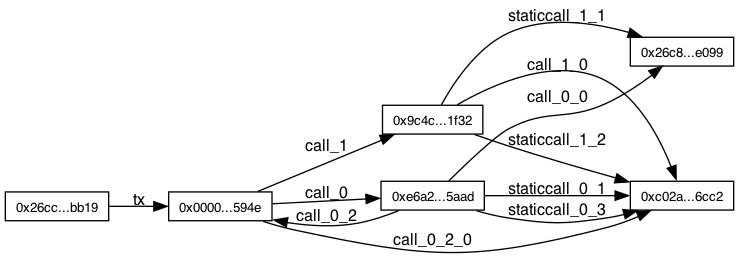
\includegraphics[width=1\textwidth]{Figures/methods/traces.png}
  \caption{Example of the structure of traces in a transaction.}
  \label{fig:traces}
\end{figure}

The only reference to the error is present in the single trace that failed, with an {\tt error} field. To understand if a deployment or the destruction successfully completed, it is necessary to propagate the error from the failed traces to all its children. Eth2dgraph does so with the algorithm reported in \cref{lst:error-propagation}. It first groups traces of a block based on transaction hash. Then, for each transaction, it gets its failed traces. Then it loops again on all the traces of the transaction to see if any of them is a child of a failed one. This is done by searching a failed trace that has a matching starting address, e.g. a trace with address {\tt 1, 0, 0} has a matching starting address of the trace {\tt 1, 0, 0, 2}.

Contract deployments and destructions found in failed traces are stored in the output of eth2dgraph with a boolean field indicating it.

\begin{lstlisting}[language=Rust,caption={Algorithm for errors propagation in traces.},label={lst:error-propagation},captionpos=b, style=boxed]
fn propagate_errors(traces: &mut Vec<Trace>) {
    // group traces by transaction hash
    let mut txs: HashMap<TxHash, Vec<&mut Trace>> = HashMap::new();
    traces.iter_mut().for_each(|t| {
        if t.transaction_hash.is_some() {
            let group = txs
                .entry(t.transaction_hash.unwrap().clone())
                .or_insert(vec![]);
            group.push(t);
        }
    });
    // inside each transaction, mark trace as failed if a parent trace has failed
    txs.iter_mut().for_each(|(_, grouped_traces)| {
        // collect trace addresses of failed traces
        let failed = grouped_traces
            .iter()
            .filter(|t| t.error.is_some())
            .map(|t| t.trace_address.clone())
            .collect::<Vec<Vec<usize>>>();
        // loop again traces to flag ones whose parent failed
        grouped_traces.iter_mut().for_each(|t| {
            let address = t.trace_address.as_slice();
            let parent_failed = failed.iter().any(|f| address.starts_with(f));
            if parent_failed {
                t.error = Some("Parent failed".to_string());
            }
        });
    });
}
\end{lstlisting}

\subsection{Accounts}

As for the smart contracts, there is no RPC to get the list of accounts used on the Ethereum blockchain. They must be extracted as they are used.

Being a permissionless blockchain implies that there is not an initial phase of registration or an official opening of an account. Users simply generate an address and start using it. 

Eth2dgraph stores accounts every time they are used in the following cases:

\begin{itemize}
    \item Senders or receivers of transactions.
    \item Receivers of validator withdrawals.
    \item Authors of blocks (miners).
    \item Receivers of SELFDESTRUCT reward.
    \item Deployer of a smart contract.
    \item Senders or receivers of token transfers.
    \item Addresses of contract deployment or destruction, marked as contracts.
    \item Addresses of contract emitting logs, marked as contracts.
    \item Addresses of a contract emitting a token transfer, marked as contract.
\end{itemize}

\section{Semantics extraction}

The previous section described how raw Ethereum data is extracted. In this section, I describe how eth2dgraph extracts semantics from this data.

The semantics extracted are meant to give a more comprehensive description of the smart contracts stored on the blockchain. The only information that can be taken from the Ethereum protocol about smart contracts is their EVM bytecode. The EVM bytecode is the byte representation of the contracts' compiled code that can be run by the Ethereum Virtual Machine implemented in all the nodes. While it is fundamental to the functioning of the protocol, it does not give any meaningful description of the smart contract for a human analysis. 

Eth2dgraph tries to put together pieces of information to allow for an easier analysis of such smart contracts.

\subsection{ABI extraction}

\label{decompilation-section}
Smart contracts are described by an \textbf{Application Binary Interface} (ABI) that lists all the functions and events that are implemented. 

Smart contracts can be seen as REST APIs. The application status is stored in the contract's private code, similar to a database.
The public functions exposed by the contract are like the API endpoints that can be used by users to interact with the application. This is done via stateless transactions (in the blockchain) and via API calls (in the traditional REST API pattern). The ABI is the description of the exposed functions, similarly to the specification of an API. 

It is clear that having the ABI of a smart contract gives many useful insights about what it does. It can also be used to decode transactions and logs. In the ABI, there are the types of functions and events arguments. These types can be used to decode the bytes present in the transactions and logs data. It is possible to understand if they represent addresses, numbers, strings, bytes, etc..

To extract the ABI, eth2dgraph integrates heimdall-rs\footnote{EVM decompiler written in Rust, source code available at: \url{https://github.com/Jon-Becker/heimdall-rs}}, an open-source EVM decompiler. Heimdall-rs uses symbolic execution to create the control flow graph (CFG) of the EVM bytecode. This is done via a custom implementation of the EVM. From the CFG, and looking at the function dispatcher part of the code, it is possible to locate functions and extract their inputs and outputs parameter types.

It is possible to extract function names using a database of reverse hashes. Function selectors are stored in the bytecode as the first four bytes of the hash of the functions' signature. It is possible to read these four bytes and see if there are matching signature that were previously reverse hashed. Heimdall-rs does this using the public etherface\footnote{Etherface is a database of Ethereum functions and event signatures, with related hashes, available at: \url{https://www.etherface.io/}} database. 
Unfortunately, it is not possible to extract parameters name from the bytecode stored on the blockchain. This piece of information is removed during the compilation of the code. 

Heimdall-rs is integrated in eth2graph using separate processes. Each time there is the need of running the decompiler, eth2dgraph creates a new process. This is done for isolation. For the nature of how the decompiler works, it can run in infinite loops during the symbolic execution. To avoid that, eth2dgraph has a parameter to set the maximum time spent waiting for de-compilation. The default is  five seconds.

The output or the heimdall-rs process is stored to text files. When decompilation is done, these files are de-serialized by eth2dgraph into Rust data structures. \cref{fig:decompilation-architecture} shows how decompilation in handled in eth2dgraph.

\begin{figure}[H]
  \centering
  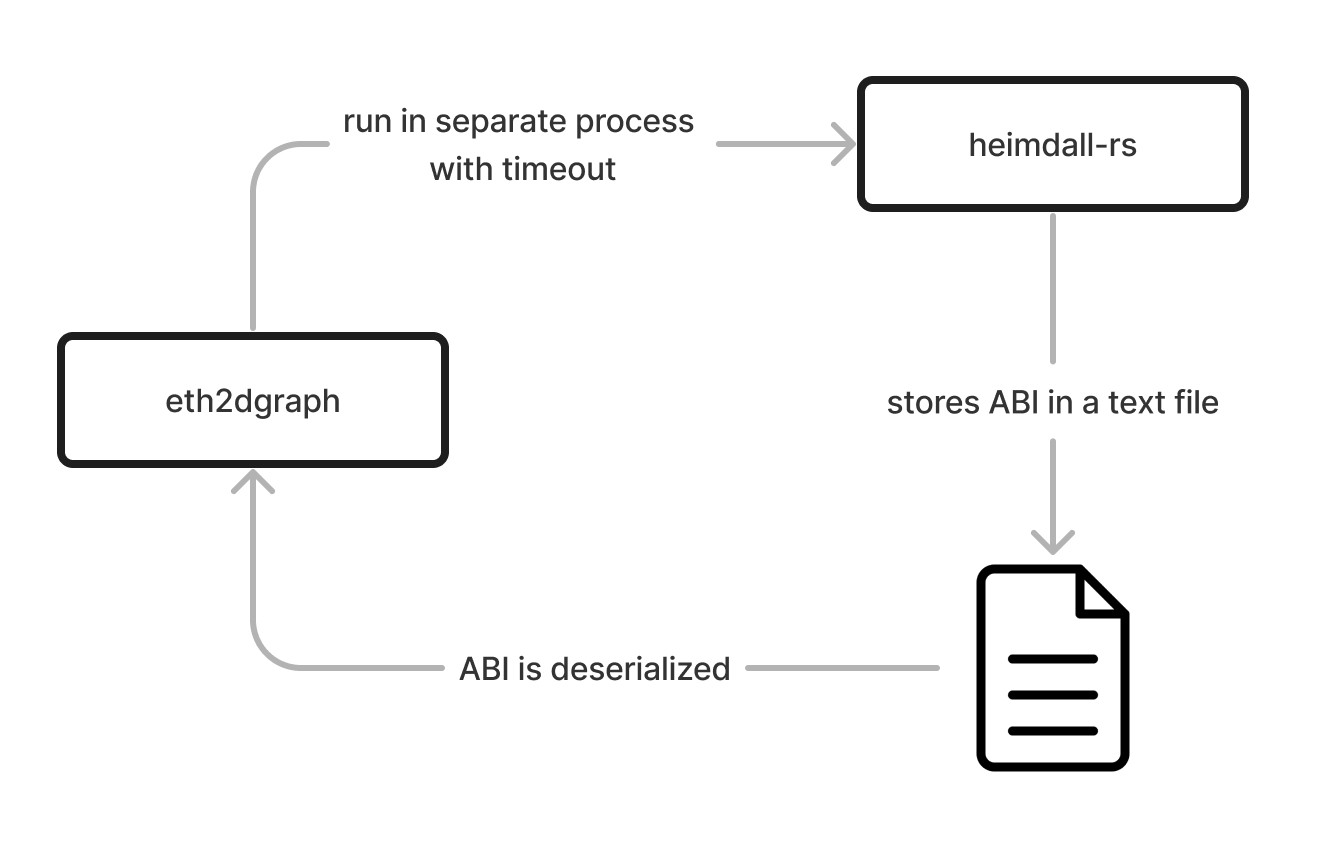
\includegraphics[width=1\textwidth]{Figures/methods/decompilation-architecture.jpg}
  \caption[Heimdall-rs integration into eth2dgraph]{Heimdall-rs integration into eth2dgraph}
  \label{fig:decompilation-architecture}
\end{figure}

\subsection{Contracts skeleton and metadata}
\label{skeleton-section}
The \textit{skeleton} of an EVM bytecode is the bytecode itself with all the arguments of the PUSH opcode set to zero. It allows to find bytecodes that are functionally identical between them. The concept of skeleton is used in many studies to reduce the total number of contracts to analyze~\cite{token-contracts}\cite{wallet-contracts}.

Removing the PUSH arguments to the bytecode deployed on the blockchain is not enough to extract the skeletons. The Solidity compiler can add metadata at the end of the bytecode that must be removed before getting the skeleton.  

Eth2dgraph identifies this part using a regular expression. Metadata is stored as CBOR\footnote{CBOR is a binary data serialization format standardized in RFC8949 \url{https://www.rfc-editor.org/rfc/rfc8949.html}} encoded data. After being splitted, the \textit{runtime} part of the bytecode is processed for the skeleton extraction, while the metadata part is decoded. Metadata are also stored in the indexed data, these are the field included:

\begin{itemize}
    \item \textit{storage\_protocol}: distributed file system protocol where the developer can eventually store the source code of the contract.
    \item \textit{storage\_hash}: location on the contract's data in the distributed file system.
    \item \textit{compiler}: the version of the Solidity compiler used.
    \item \textit{experimental}: whether the compilation was performed with experimental features activated.
\end{itemize}

The skeleton extraction is performed by looping trough the bytes of the EVM bytecode. A byte between \texttt{0x60} and \texttt{0x7f} represents a PUSH instruction. If a byte is found in that range, the next bytes are replaced with zeros depending on the kind of PUSH found. 

\subsection{Verified source code}

It is possible to link contracts to their verified source code using the repository of \textit{Smart Contract Sanctuary}~\cite{smart_contract_sanctuary}. After cloning the repository locally, eth2dgraph can be ran with an option to include source code of the discovered contracts in the indexed data.

This allows querying the contracts based on text inside the source code. Dgraph supports text matching with stemming stop words removal. Data can be queried with two query functions: \texttt{anyoftext} and \texttt{alloftext}.

\subsection{Token transfers}

The ERC20 and ERC721 token standards states that when a token ownership is transferred an event MUST be emitted. \cref{lst:erc20-transfer} shows the event emitted for fungible token transfers, \cref{lst:erc721-transfer} shows the one emitted for NFT transfers. Emitting an event means generating a log that is indexed by Ethereum nodes.

\begin{lstlisting}[caption={Event emitted for ERC20 token transfer},label={lst:erc20-transfer},captionpos=b]
event Transfer(address indexed _from, address indexed _to, uint256 _value)
\end{lstlisting}

\begin{lstlisting}[caption={Event emitted for ERC721 token transfer},label={lst:erc721-transfer},captionpos=b]
event Transfer(address indexed _from, address indexed _to, uint256 indexed _tokenId)
\end{lstlisting}

Both events share the same name and types. The only difference is in the last parameter. It is indexed in case of ERC721 and not indexed in case of ERC20. The signature of the event is not influenced by this difference, so all the logs that are describing token transfers share the same signature.

Logs with the first topic matching the keccak256 hash of the Transfer event signature are treated as token transfer by eth2dgraph.

After finding a matching log, the bytes composing the data field are split into 256 bit words and merged to the 256 words of the indexed topics.

The 256 bit words are then treated and decoded as follows:

\begin{itemize}
    \item First word is the \textit{from} address.
    \item Second word is the \textit{to} address.
    \item Third word is the \textit{value}. It represent the amount in case of ERC20 or the token ID in case of ERC721.
\end{itemize}

If the decoding succeeds, the log is parsed and later stored as a token transfer.

Distinction between ERC20 and ERC721 transfers is done based on length of the topics array. Since ERC20 has the last parameter not indexed, the topics length is three words. For the ERC721 the topics length is four. This information is used to discriminate between storing the third word as \textit{value} or as \textit{token\_id}.

The same way of semantics extraction can be used for other kind of logs, e.g. token swaps. Eth2dgraph implements the code for parsing token transfer since it is the most common log emitted on the Ethereum chain.

\section{Software architecture}

The Ethereum network stores data in the order of billions of entries. The process of extraction must be as efficient as possible to be able to get this data in reasonable time. At the time of writing, Ethereum has 17.5M blocks. Performing each single action described in the previous sections sequentially for each block results in executions that take many days or even weeks. 

A lot of time is spent waiting for network data (the calls to the RPCs) or for the decompiler process to complete the decompilation. While it is not possible to make these steps faster, it is possible to parallelize them. Eth2dgraph has been developed to maximize concurrency of the machine where it is ran to minimize the time needed for data extraction.

This was done using async Rust and the \textit{Tokio asyncronous runtime}\footnote{Tokio provides a multi-threaded runtime for executing asynchronous Rust code \url{https://tokio.rs/}.}. \cref{fig:eth2dgraph-architecture} gives a general overview of how tasks are used and how they communicate.

\begin{figure}[H]
  \centering
  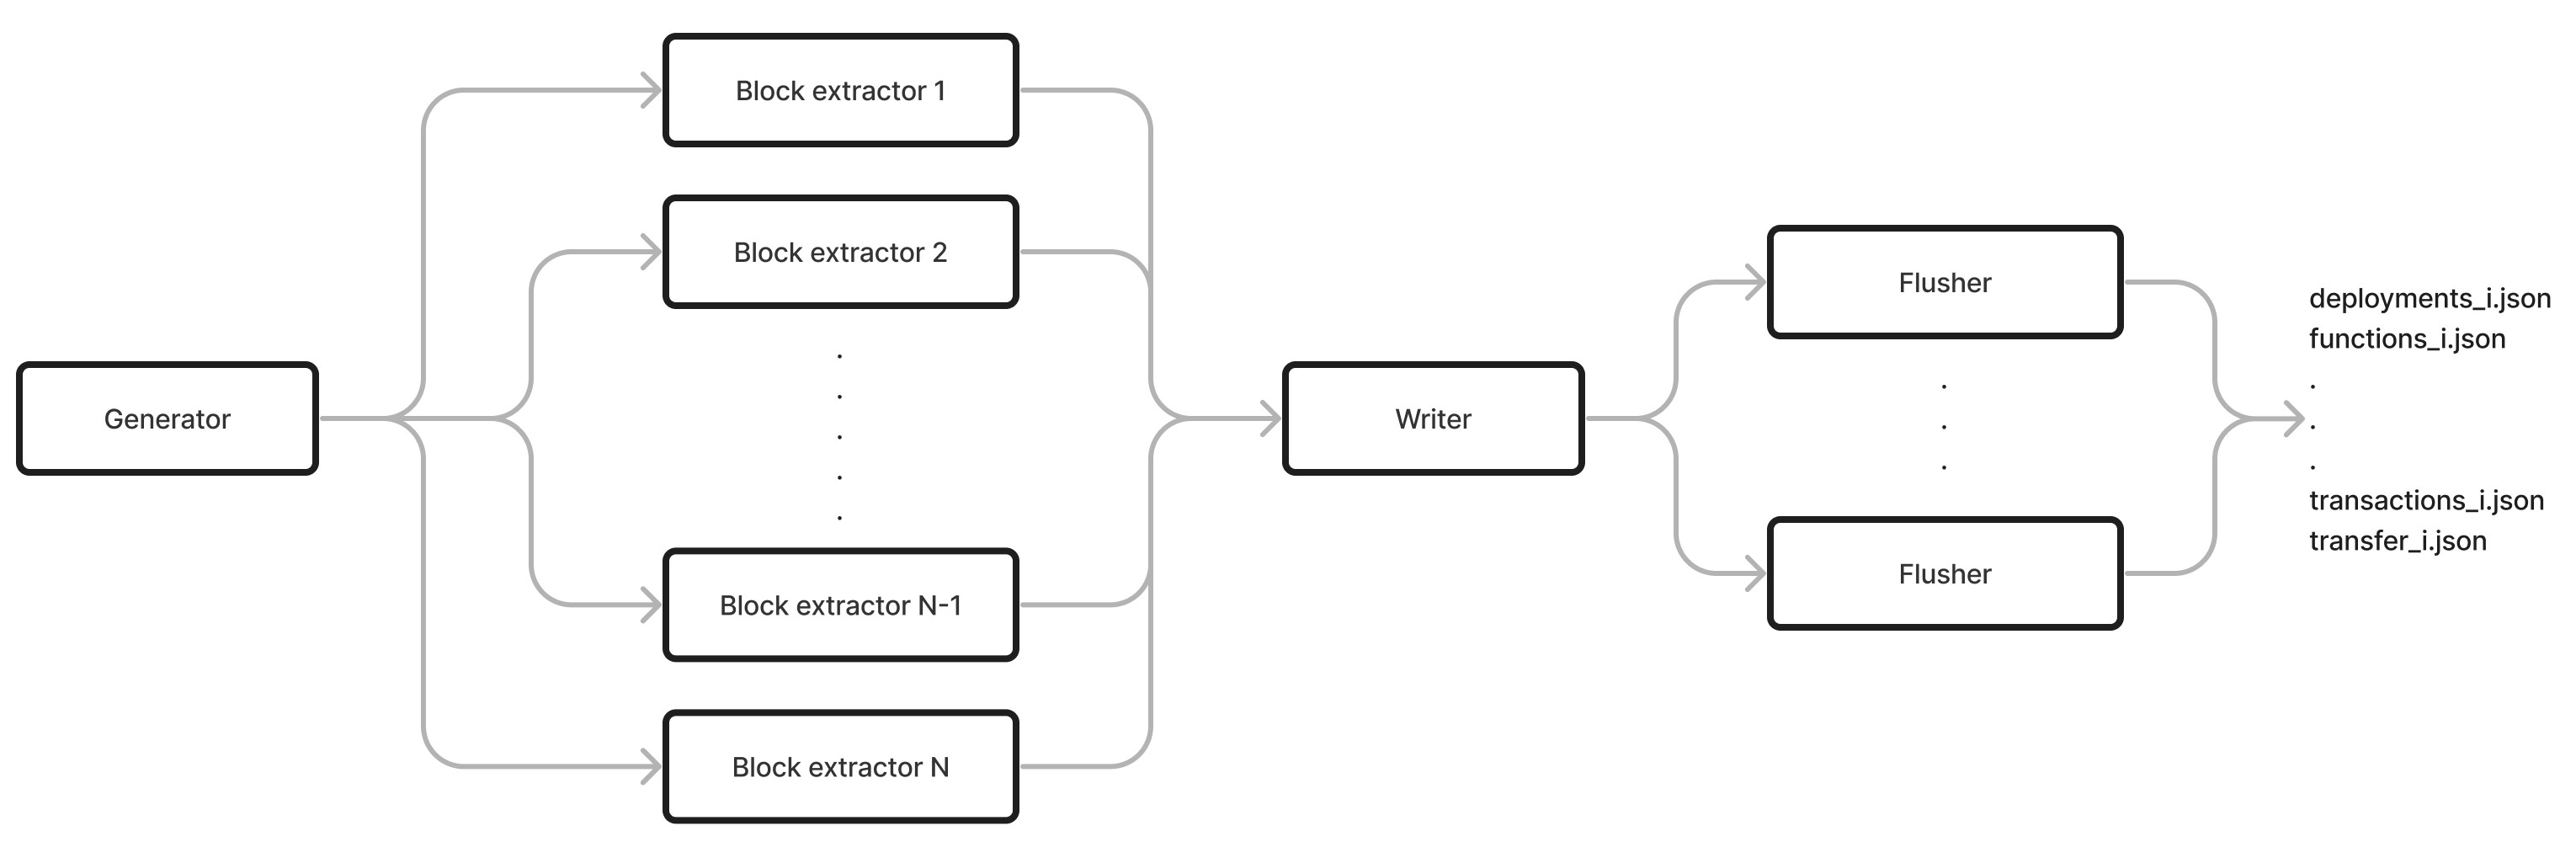
\includegraphics[width=1\textwidth]{Figures/methods/software-architecture.jpg}
  \caption[Software architecture of eth2dgraph]{Software architecture of eth2dgraph}
  \label{fig:eth2dgraph-architecture}
\end{figure}

Here is a more detailed description of each task:

\begin{itemize}
    \item The \textit{generator} task loops trough the block range to extract and spawns, using \texttt{tokio::spawn}, an \textit{extractor} task for each block that must be processed. It is also responsible for initializing all the data structures needed, the output data folders and the \textit{writer} task. 
    
    It is possible to set the limit of parallel extractor tasks to run usign the \texttt{--num-jobs} option. This is implemented using a semaphore. Each time an extractor task is created, it acquires a permit from a semaphore with a fixed capacity. When the task ends, the permit is dropped and, as a consequence, a new permit is freed in the semaphore. In case the maximum number of tasks is reached, the generator waits until the semaphore has a free permit available. This was done to avoid overloading the system with millions of concurrent tasks.

    \item The extractor task is the one responsible for the actual extraction. It receive as an argument the block to process and it collects all the data related to it. This includes handling the decompilation. All the steps related to data extraction were described in the previous sections.

    When data is ready to be stored, it is sent to the writer task using a bounded \textit{multiple-producer single-consumer} (mpsc) channel.

    \item The writer task is responsible to collect all the data sent by all the extractors and merge it. It stores data in buffers, one for each data type. When buffers reach a certain size, that can be set with the \texttt{--size-output} option, they are sent to a \textit{flusher} task to be stored to disk. The flusher tasks are spawned on demand by the writer task using \texttt{tokio::spawn\_blocking}. All their join handles are stored in a vector to wait for their termination at the end of the extraction.

    \item The flusher task is responsible for storing and compressing the output of the extraction. It receives a vector of a generic type \texttt{T} that implements the trait \texttt{SerializeDgraph}. It compresses this vector using gzip with a compression level that can be set as an option. Finally, it stores it in an output file. Data is stored divided by type and with incremental file names.
\end{itemize}

All these tasks are ran on the multi-threaded Tokio runtime. They are managed by the Tokio scheduler that implements a \textit{non-preemptive}, also called \textit{cooperative}, scheduling strategy. This means that tasks are switched when they explicitly ask for it, giving back the control to the scheduler. 

In this way it is possible to maximize the parallelism of the extraction process. For example, when a task is downloading block's data, it calls \texttt{await} on the library function responsible for networking. This call tells the Tokio scheduler that the task is paused and cannot continue, so it is replaced with another task that has work to do.

\subsection{Decompilation cache}
\label{cachine-section}
One of the biggest bottlenecks of the extraction process was the decompilation step. Spawning a dedicated process for handling decompilation of each contract deployment takes a lot of time. The main problem is that the decompiler, for how it is designed, can encounter infinite loops during the building of the control flow graph. To avoid that, it is ran with a timeout of a few seconds, but even with that, it was slowing down the process by a lot.

The solution implemented in eth2dgraph is caching the decompilation based on bytecode skeletons. Two contract deployments sharing the same EVM skeleton are decompiled only once. The decompiled ABI of a skeleton comes from the decompilation of the first contract found with that skeleton.

The reason of this choice is that contracts sharing the same skeleton also share the same code logic. In theory, there could be a difference in the function names, since they are stored as arguments of PUSH instructions, but, from the data analyzed, this almost never happens.

To test the reliability of the caching logic, I compared ABIs extracted from decompiling each single contract to the ones got using the cache. To make the test more reliable, I ran it on various block ranges spanning trough the history of the Ethereum blockchain. \cref{table:caching-precision} reports the results of the tests. Full match means that the ABI got from the cache is exactly the same as the one got from a new decompilation run. Partial match indicates that the ABI got from the cache has the same exact function and event names, but there is at least one difference between types based on assumptions made by the decompiler (e.g. bytes instead of address). Mismatch indicates that the ABI got from the cache has at least one different function or event name.

\begin{table}[ht!]
\centering
    \begin{threeparttable}
    \begin{tabular}{m{3cm} m{2cm} m{2cm} m{2cm} m{2.5cm}} 
    \toprule
    \textbf{Blocks range} & \textbf{Cache hits} & \textbf{Full matches} & \textbf{Partial matches} & \textbf{Mismatches}   \\
    \midrule
    6000000-6001000   & 1373 & 1373 & 0 & 0 \\
    10000000-10001000 & 596 & 592 & 4 & 0 \\
    12008000-12009000 & 1296 & 1295 & 1 & 0 \\
    15505000-15506000 & 101 & 101 & 0 & 0 \\
    16001000-16002000 & 120 & 100 & 19 & 1 \\
    17000000-17001000 & 39 & 39 & 0 & 0 \\
    \bottomrule
    \end{tabular}
    \end{threeparttable}
    \caption{Precision of the decompilation caching logic}
    \label{table:caching-precision}
\end{table}

In total, 99.29\% of the cache hits resulted in full matches, 0.68\% in partial matches and just 0.03\% in mismatches.

This level of accuracy showed that caching decompilation based on skeletons is an effective way of reducing the time needed for semantics extraction. The slight loss of precision is justified by the boost in performance, that made it possible to scale the extraction of ABIs to all the history of the chain in a single machine. It allowed to reduce the number of decompilation runs from 60M to 470k.

The cache is implemented in the code with a shared \texttt{HashMap}. The implementation of the concurrent hashmap used is the one provided by the {\tt DashMap}\footnote{DashMap provides a concurrent hashmap that is faster and easier to use that the combination of {\tt RwLock} and {\tt HashMap}. It is available at:\url{https://github.com/xacrimon/dashmap}} crate. The \textit{key} of the hashmap is the hash of the skeleton's bytecode and the \textit{value} is an \textit{atomic unsigned integer}. The role of the number in the cache is of indicating how many failures that specific skeleton has encountered during decompilation. It is used for trying multiple times to decompile a skeleton that fails to decompile even with different contracts' bytecodes. These is an hard limit of ten attempts, after which the skeleton is stored without the ABI and no more decompilation processes will be spawned.

This way of extracting semantics has a direct implication on the schema of data. The ABI extracted by the decompiler is linked to the skeleton and not to the contract deployment itself. \cref{fig:contracts-storage} shows the result of this design choice in the schema.

\begin{figure}[H]
  \centering
  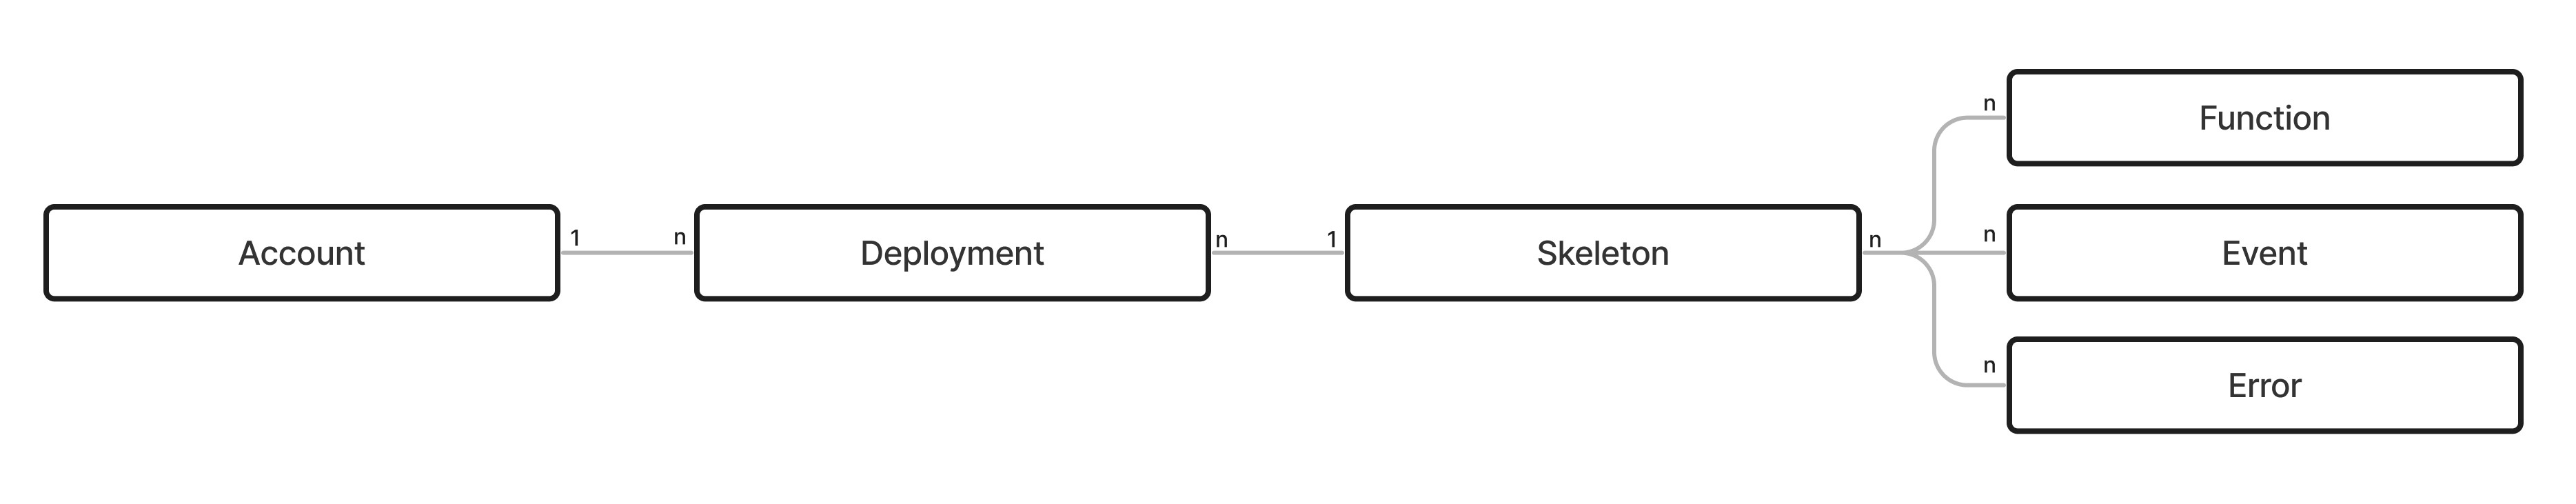
\includegraphics[width=1\textwidth]{Figures/methods/contracts-storage.jpg}
  \caption[Storage of contracts' information]{Storage of contracts' information}
  \label{fig:contracts-storage}
\end{figure}

\section{Similarity calculation}
\label{similarity-calculation}
Smart contracts' deployments are clustered based on bytecode skeletons: many smart contracts share the same skeleton and thus they are linked to the same skeleton's entity in the database. To link these skeleton clusters together, some similarity metrics are needed. Linking skeleton clusters helps the process of data analysis; it ease the recognition of patterns and connections.

Eth2dgraph implements two similarity metrics:

\begin{itemize}
    \item \textit{Interface similarity}: inspired by Di Angelo and Salzer \cite{clustering-sc}, it calculates similarity between skeletons as the Jaccard index of the sets of function and event names. Two skeletons are similar if they have similar ABIs. It is calculated as 
    \begin{equation}
	Sim = \frac{|A\cap B|}{|A\cup B|}
    \end{equation}
    where $A$ and $B$ are the sets containing function and event names. It gives a number between $1$ (identical ABIs) and $0$ (non-overlapping ABIs).
    
    \item \textit{Bytecode similarity}: The interface similarity logic works greatly if the smart contracts implement many public functions, but it doesn’t work very well if most of the code lies in internal functions and the exposed ones are just a few, like \texttt{start()} or \texttt{run()}. 
    To face this problem I added a second similarity metric that just considers the contracts' bytecodes. Inspired by Kiffer et al.~\cite{ethereum-sc-topology}, the metric used is the cosine similarity between hypervectors containing the frequencies of opcodes' 5-grams. It is computed as follows:
    \begin{enumerate}
        \item The two bytecodes to analyze are decoded to extract the opcodes, without their arguments.
        \item From the opcodes, the 5-grams and their frequencies are calculated. For example these instructions: 
        \begin{lstlisting}
PUSH1
PUSH1
MSTORE
CALLVALUE
DUP1
ISZERO
PUSH2
JUMPI
PUSH1\end{lstlisting}
        give these 5-grams with related frequencies:
        \begin{lstlisting}
[
    ("PUSH1 PUSH1 MSTORE CALLVALUE DUP1", 1),
    ("PUSH1 MSTORE CALLVALUE DUP1 ISZERO", 1),
    ("MSTORE CALLVALUE DUP1 ISZERO PUSH2", 1),
    ("CALLVALUE DUP1 ISZERO PUSH2 JUMPI", 1),
    ("DUP1 ISZERO PUSH2 JUMPI PUSH1", 1),
]       \end{lstlisting}
        \item This results in having two hypervectors, here called $A$ and $B$, in the dimension of the 5-grams. The cosine similarity is the cosine of the angle between these two vectors. It is possible to compute it as 
        \[
        cos(\theta)=\frac{A \cdot B}{||A||\,||B||}=\frac{\sum\limits_{i=1}^{n}A_iB_i}{ \sqrt{\sum\limits_{i=1}^{n}A^2_i \cdot \sum\limits_{i=1}^{n}B^2_i} }
        \]
        This gives a number between 0 (completely dissimilar bytecodes) and 1 (identical bytecodes). The suggested threshold for considering similarity suggested by Kiffer et al. is of $0.90$.
    \end{enumerate}
\end{itemize}

The process of similarity calculation is done on demand after data is loaded into Dgraph. The same binary that is responsible for the data extraction part also integrates commands to perform data analysis. 

It is possible to run eth2dgraph with the \texttt{analyse similarity} command to calculate both the previous metrics. Comparing all skeletons with each other is a heavy calculation, with a quadratic complexity with respect to the number of skeletons. It is possible to restrict the calculation to a single skeleton, giving as an argument the address of a contract.

To optimize the performances, calculation of similarity is done in parallel using the \textit{parallel iterators} of the \textit{Rayon}\footnote{Rayon is a data-parallelism library that easily introduces parallelism into existing sequential code  \url{https://docs.rs/rayon/latest/rayon/}} crate.

The output of the calculation is a text file containing the RDF triples that describe the similarities. It is possible to import it into the live database by running a mutation or using the Dgraph's \textit{live loader}.

Similarity values are stored as edge attributes, called \textit{facets} in Dgraph. It is possible to query the data filtering by similarity value. \cref{lst:skeleton-similarity-query} shows an example of how to retrieve similar skeletons filtering by similarity value.

\begin{lstlisting}[caption={Example DQL query for getting similar skeletons.},label={lst:skeleton-similarity-query},captionpos=b]
{
    q(func: uid(0x180c753f6)) {
        Skeleton.similar_code @facets(gt(similarity, 0.95)) @facets(similarity) {
            uid
        }
        Skeleton.similar_interface @facets(gt(similarity, 0.95)) @facets(similarity) {
            uid
        }
    }
}
\end{lstlisting}
\cleardoublepage


\chapter{Results}
\label{chapter-5}

\section{Infrastructure used}

Eth2dgraph was developed and used on a server provided by the Decentralised Systems Engineering Lab of NTNU University\footnote{Decentralised
Systems Engineering Lab \url{https://www.ntnu.edu/idi/dse}}. The server's specifications are reported in \cref{table:server-specs}.

\begin{table}[ht!]
\centering
    \begin{threeparttable}
    \begin{tabular}  { m{3cm} m{6cm} } 
    \toprule
    \textbf{Parameter} & \textbf{Value}   \\
    \midrule
    CPU    &    64 cores, 256 threads \\[1.3ex]
    RAM    &    1.5 TB \\[1.3ex]
    OS    &     Ubuntu 22.04 \\[1.3ex]
    Disk    &   16 TB SSD array \\[1.3ex]
    \bottomrule
    \end{tabular}
    \end{threeparttable}
\caption[Specification of the server used for the work]{Specification of the server used for the work.}
\label{table:server-specs}
\end{table}

On the same machine, there was an archive Ethereum node that was used to get the data. The RPC calls did not have to go through the network, all the process was done in a single machine. The client used was Erigon\footnote{Erigon is an Ethereum client written in Go \url{https://github.com/ledgerwatch/erigon}}. It was run with the command reported in \cref{lst:erigon-command} and the RPC daemon with the command reported in \cref{lst:rpc-command}.

\begin{lstlisting}[language=bash,caption={Erigon command},label={lst:erigon-command},captionpos=b,numbers=none]
erigon \
    --datadir="our data location" \
    --chain=mainnet \
    --authrpc.jwtsecret="JWT secret location"\
    --private.api.addr=0.0.0.0:9090 \
    --http.api=eth,debug,net,trace,web3,erigon
\end{lstlisting}

\begin{lstlisting}[language=bash,caption={RPC daemon command},label={lst:rpc-command},captionpos=b,numbers=none]
rpcdaemon \
    --datadir="our data location" \
    --http.addr=0.0.0.0 \
    --http.api=eth,debug,net,trace,web3,erigon
\end{lstlisting}

\subsection{Benchmark of the Erigon's RPC interface}

To give a clearer overview of the environment in which data extraction was done, I performed a load test against the Erigon node using a modified version of \textit{flood}\footnote{Flood is an open-source tool for load testing Ethereum nodes \url{https://github.com/paradigmxyz/flood}}. I tested the throughput and the success rate, varying the requests per second, of the three RPCs used by eth2dgraph: {\tt eth\_getBlockByNumber}, {\tt eth\_getLogs} and {\tt trace\_block}. Flood was modified to generate RPC calls with the exact same parameters used by eth2dgraph, spread over random block numbers. The actual network calls were performed by \textit{vegeta}\footnote{Vegeta is a tool written in Go for load testing HTTP services \url{https://github.com/tsenart/vegeta}}, that is specifically designed to measure HTTP services with a constant request rate. Each load test was conducted for 30 seconds. \cref{fig:logs-success,fig:logs-throughput,fig:blocks-success,fig:blocks-throughput,fig:traces-success,fig:traces-throughput}~show the results of this test. The slowest RPC, and so the bottleneck of data extraction, resulted to be {\tt trace\_block}. 

% LOGS
\begin{figure}[H]
    \centering
    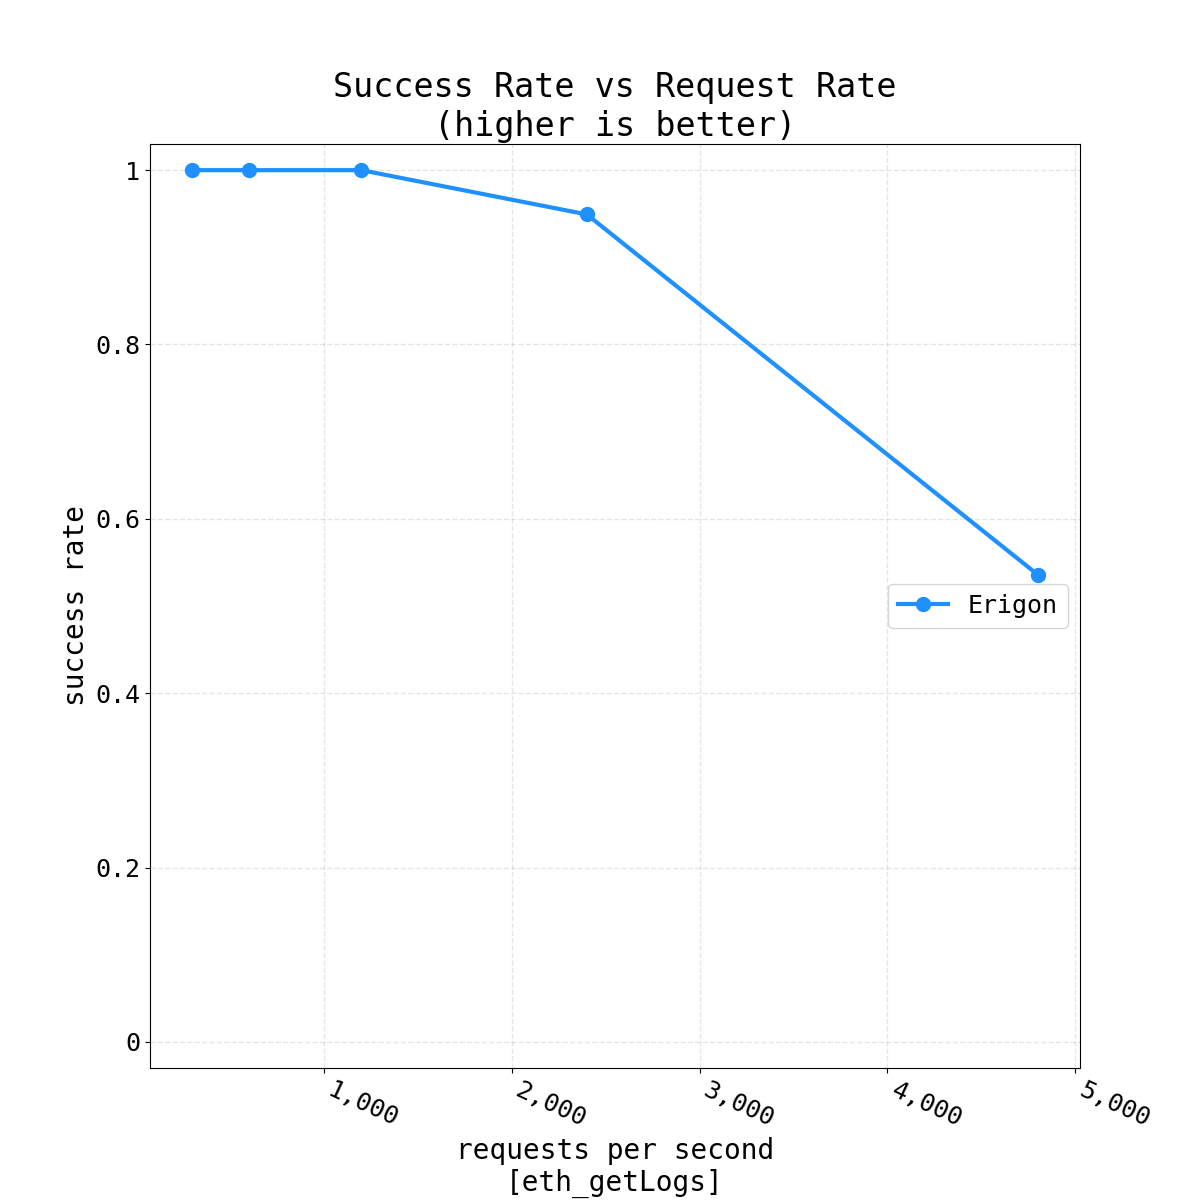
\includegraphics[width=0.7\textwidth]{Figures/results/load_tests/logs/success_rate_logs.png}
    \caption{Success rate of {\tt eth\_getLogs}. After 1200 requests/s, Erigon starts to fail handling some requests. At 5k requests/s half of the requests fail. }
    \label{fig:logs-success}
\end{figure}

\begin{figure}[H]
    \centering
    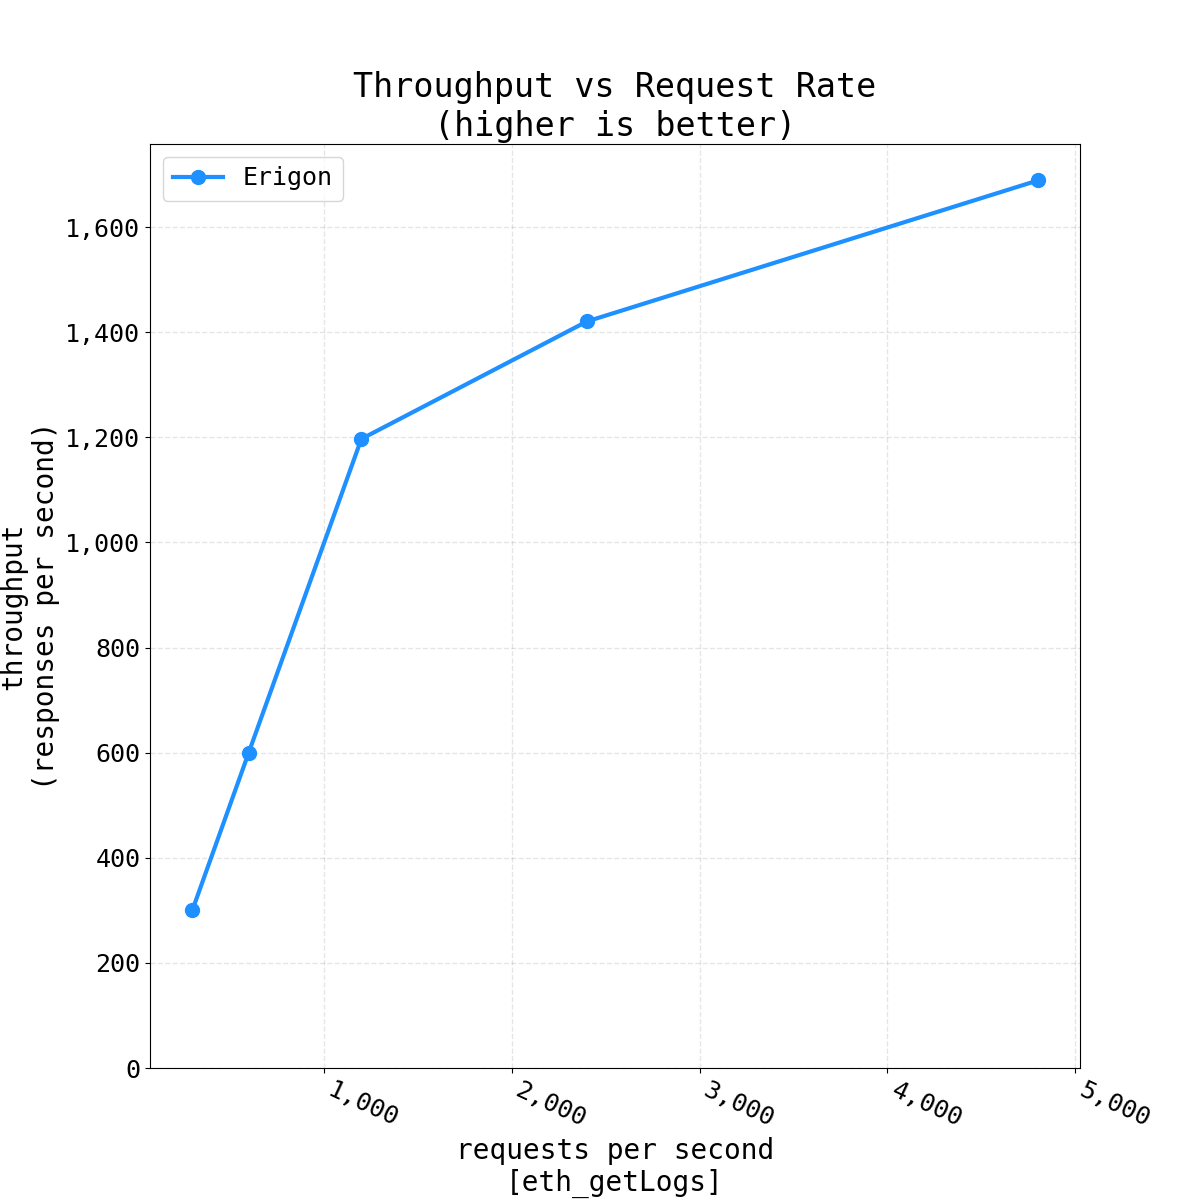
\includegraphics[width=0.7\textwidth]{Figures/results/load_tests/logs/throughput_logs.png}
    \caption{Throughput of {\tt eth\_getLogs}. After 1200 requests/s Erigon can't keep the requests rate. }
    \label{fig:logs-throughput}
\end{figure}

% BLOCKS    
\begin{figure}[H]
    \centering
    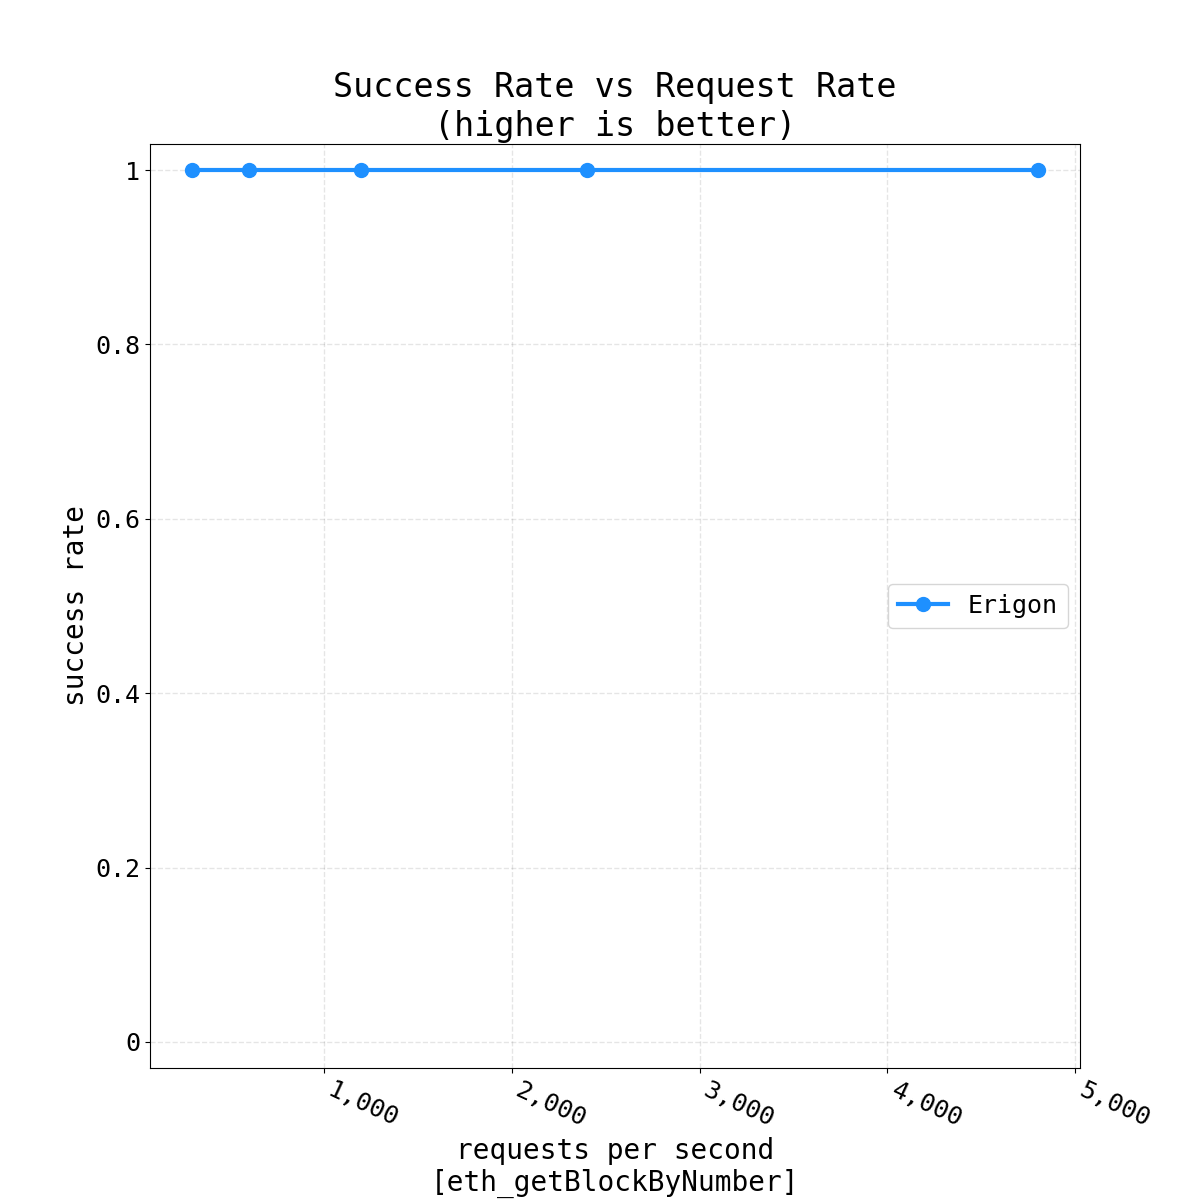
\includegraphics[width=0.7\textwidth]{Figures/results/load_tests/blocks/success_rate_blocks.png}
    \caption{Success rate of {\tt eth\_getBlockByNumber}. Erigon shows perfect performance on this RPC. It can successfully reply to 5k requests/s. }
    \label{fig:blocks-success}
\end{figure}

\begin{figure}[H]
    \centering
    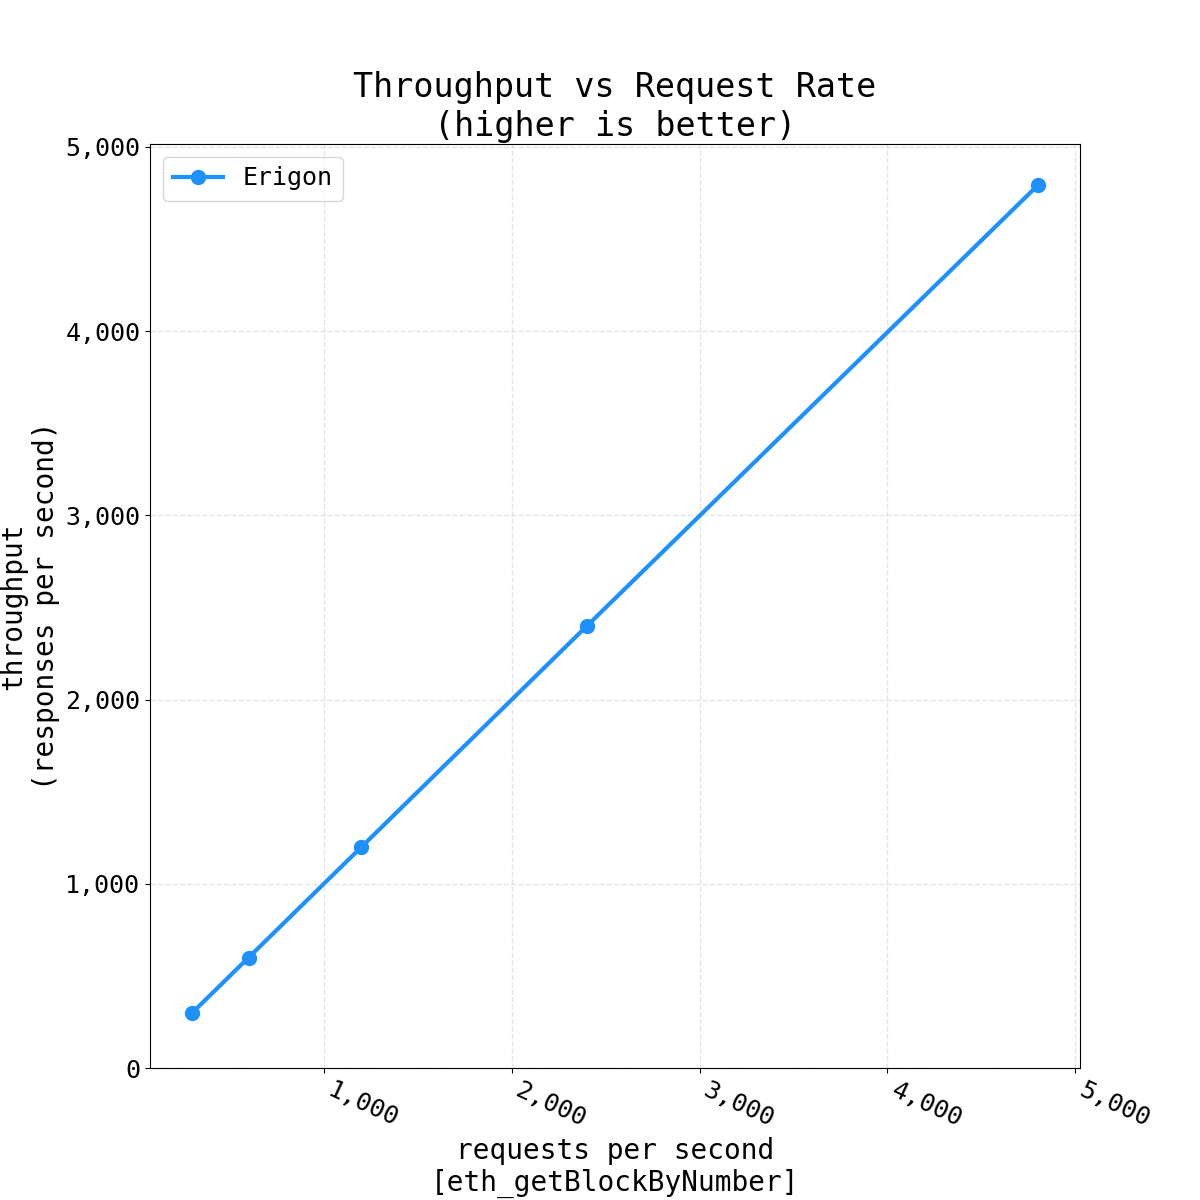
\includegraphics[width=0.7\textwidth]{Figures/results/load_tests/blocks/throughput_blocks.png}
    \caption{Throughput of {\tt eth\_getBlockByNumber}. Erigon can keep the throughput even at 5k requests/s.  }
    \label{fig:blocks-throughput}
\end{figure}

% TRACES    
\begin{figure}[H]
    \centering
    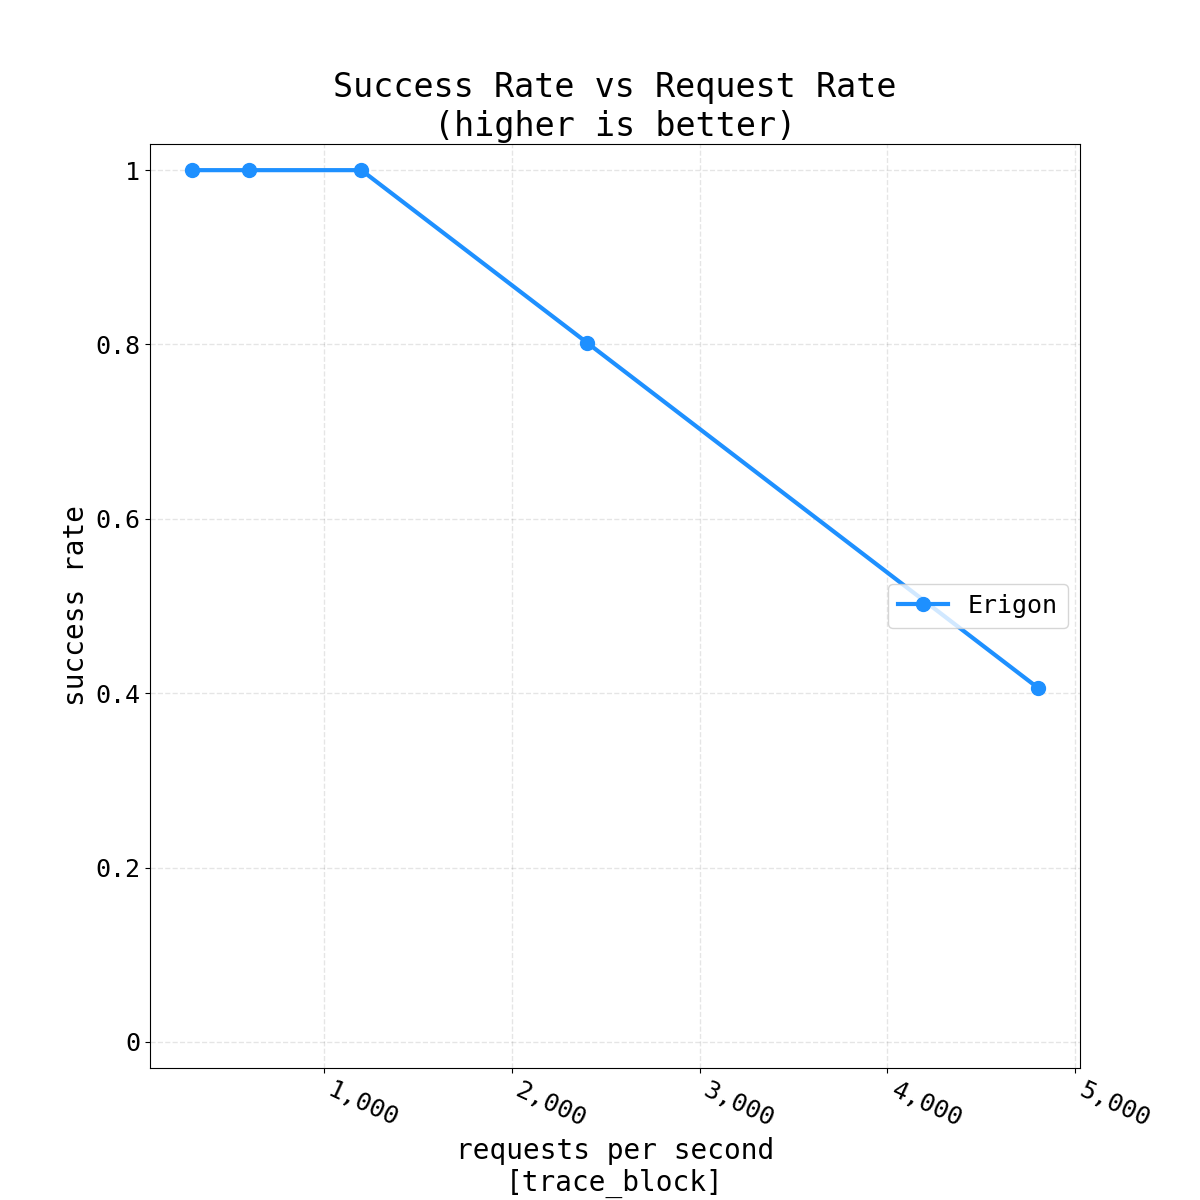
\includegraphics[width=0.7\textwidth]{Figures/results/load_tests/traces/success_rate_trace.png}
    \caption{Success rate of {\tt trace\_block}. Erigon starts to degrade after 1200 requests/s. At 5k requests/s, just 40\% of the requests are successfully handled.  }
    \label{fig:traces-success}
\end{figure}

\begin{figure}[H]
    \centering
    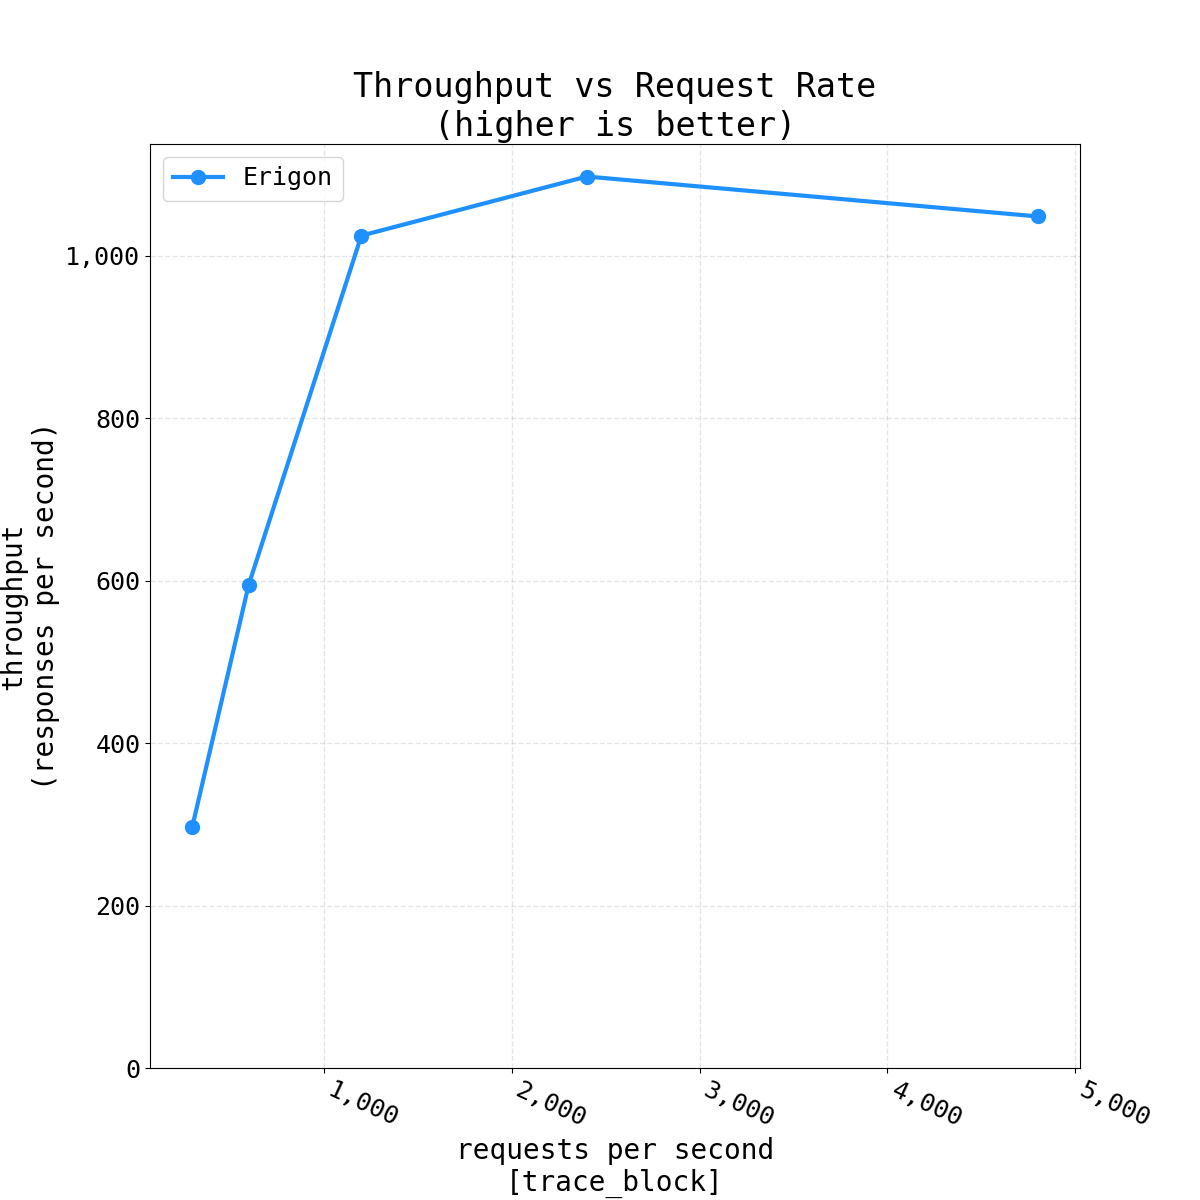
\includegraphics[width=0.7\textwidth]{Figures/results/load_tests/traces/throughput_trace.png}
    \caption{Throughput of {\tt trace\_block}. It reaches the maximum of around 1200 responses/s at 2400 requests/s. }
    \label{fig:traces-throughput}
\end{figure}

\begin{comment}

\begin{figure}[H]
    \centering
    \subfigure[]{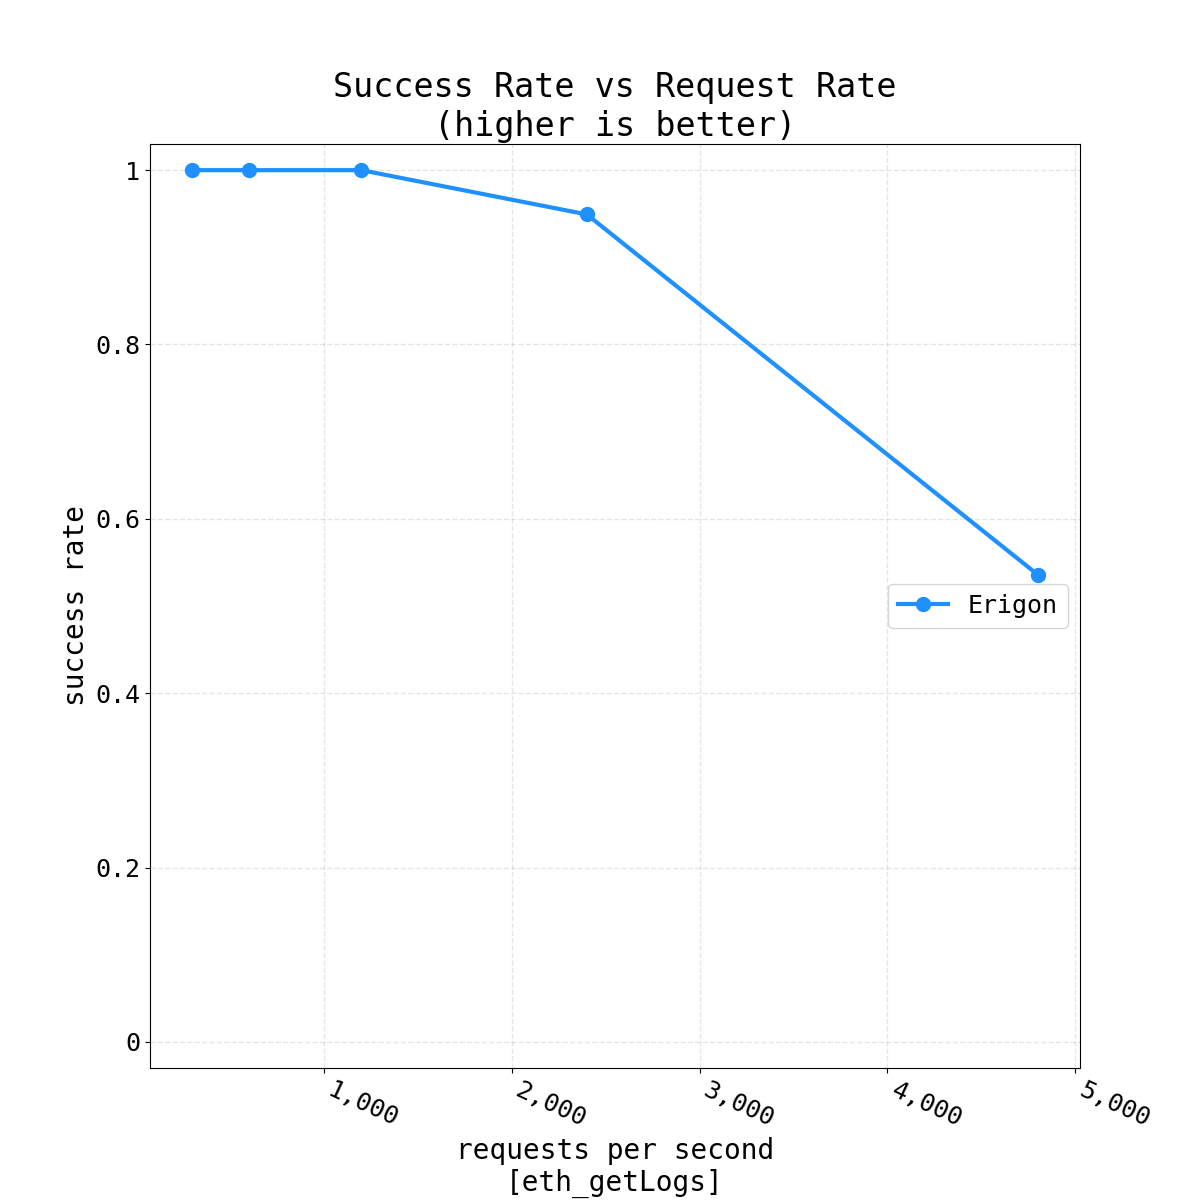
\includegraphics[width=0.48\textwidth]{Figures/results/load_tests/logs/success_rate_logs.png}} 
    \subfigure[]{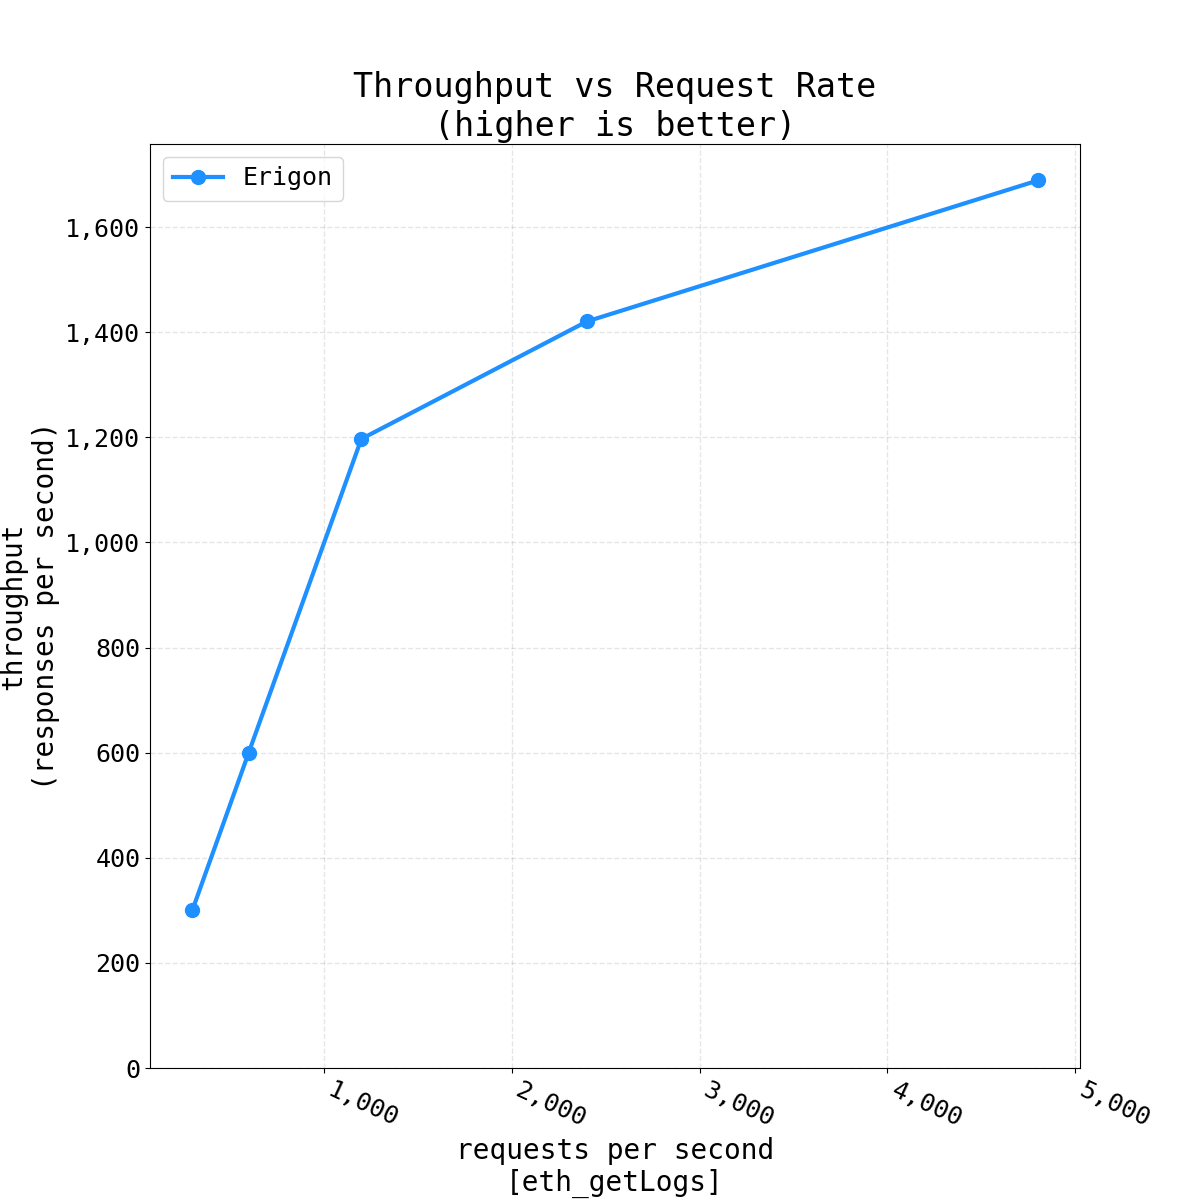
\includegraphics[width=0.48\textwidth]{Figures/results/load_tests/logs/throughput_logs.png}} 
    \subfigure[]{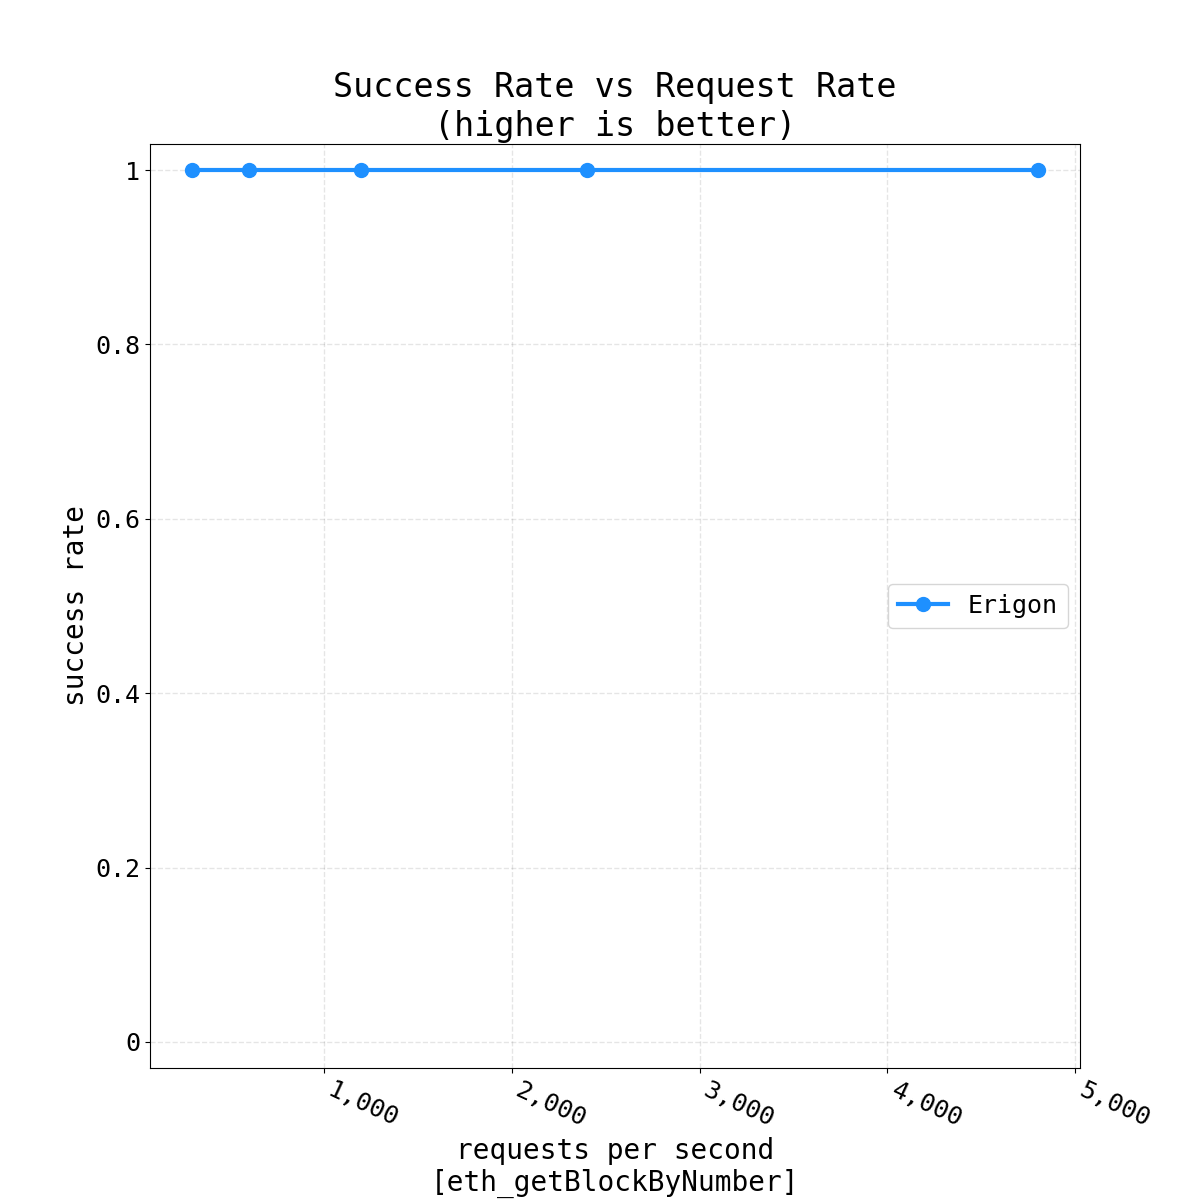
\includegraphics[width=0.48\textwidth]{Figures/results/load_tests/blocks/success_rate_blocks.png}}
    \subfigure[]{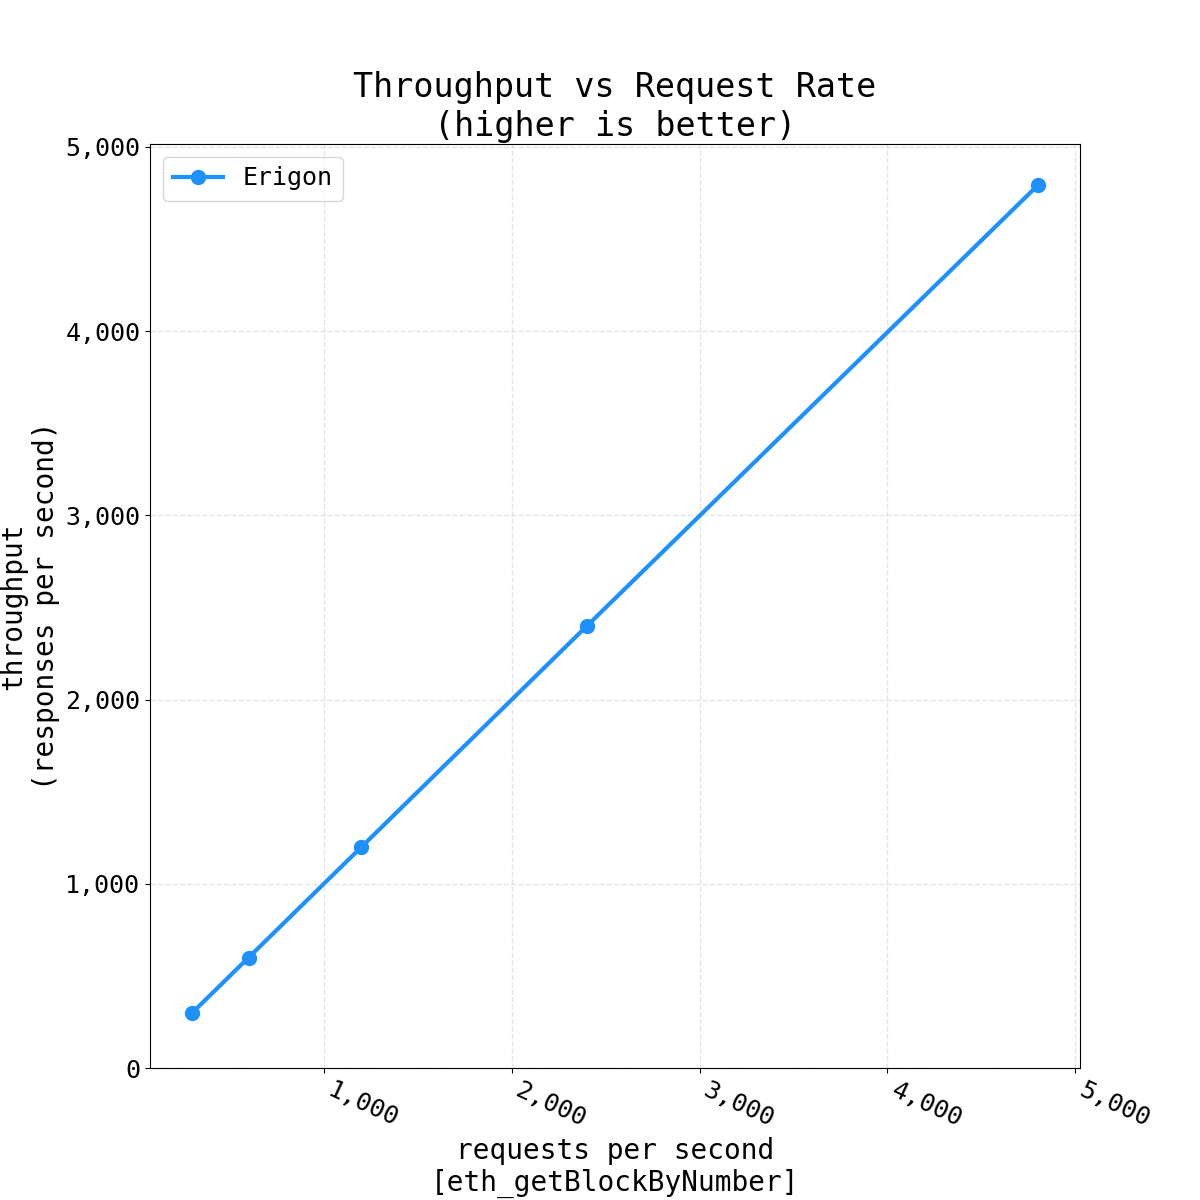
\includegraphics[width=0.48\textwidth]{Figures/results/load_tests/blocks/throughput_blocks.png}}
    \subfigure[]{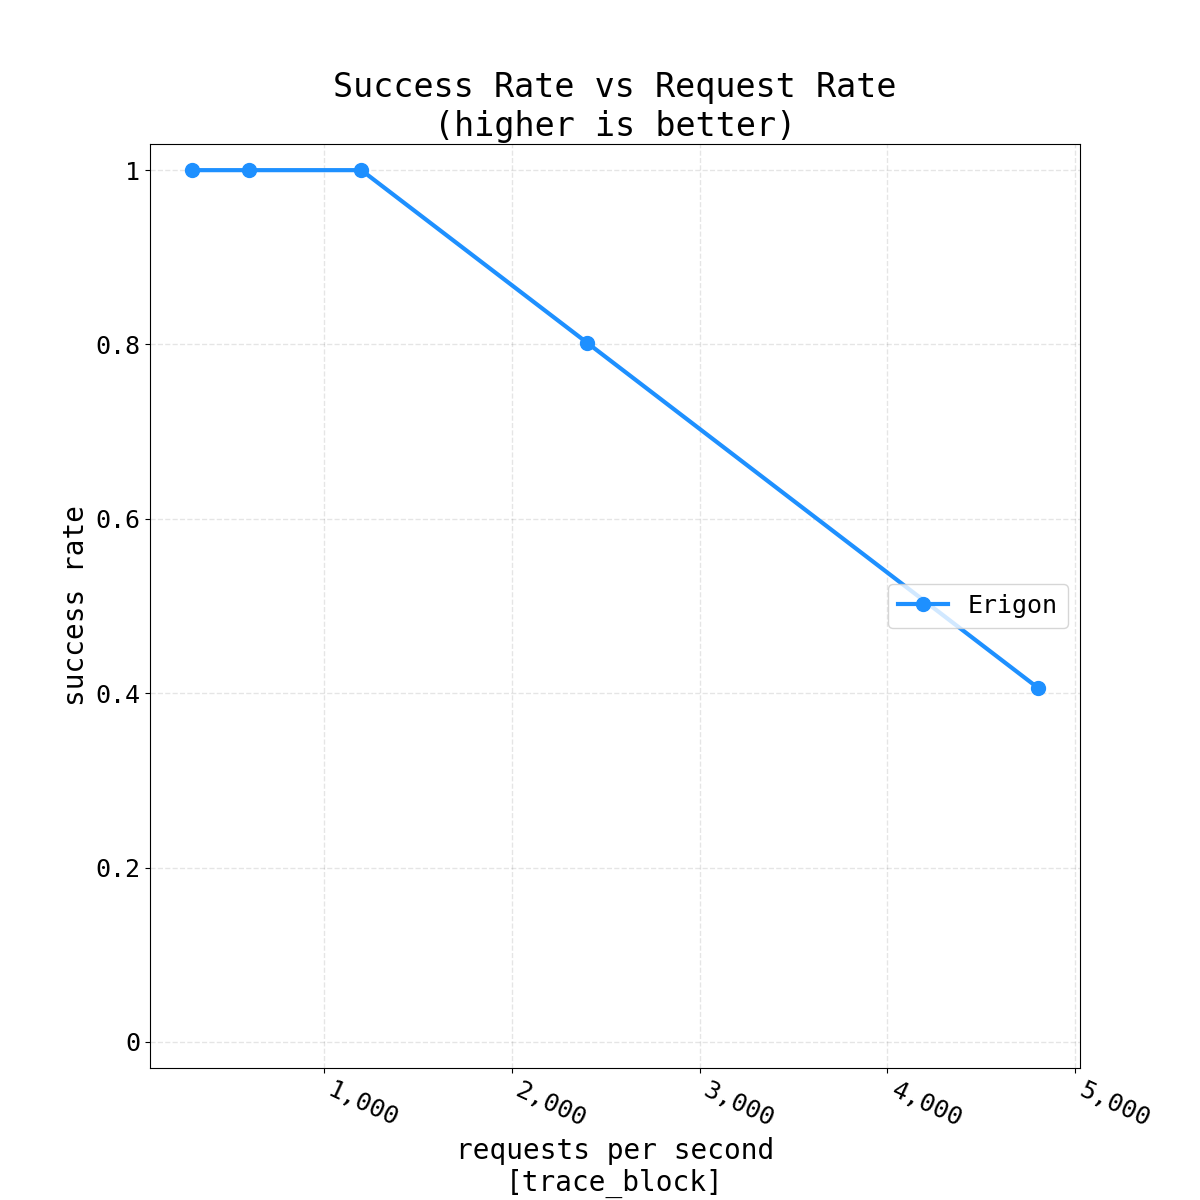
\includegraphics[width=0.48\textwidth]{Figures/results/load_tests/traces/success_rate_trace.png}}
    \subfigure[]{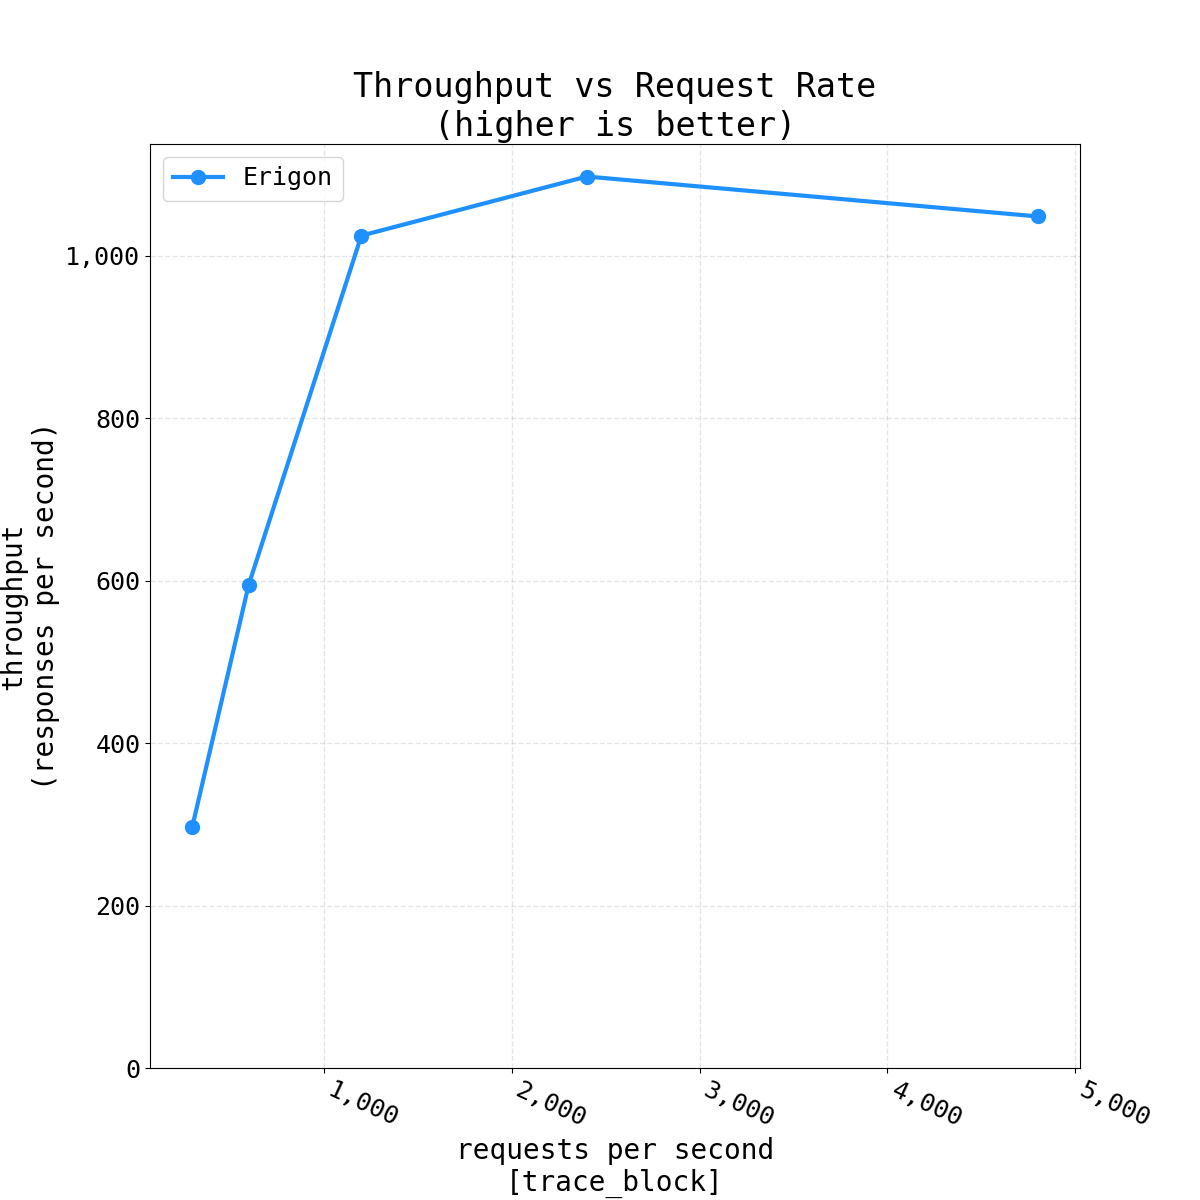
\includegraphics[width=0.48\textwidth]{Figures/results/load_tests/traces/throughput_trace.png}}
    \caption{Results of the load test for {\tt eth\_getLogs} (a, b), {\tt eth\_getBlockByNumber} (c, d) and {\tt trace\_block} (e, f).}
    \label{fig:load-test-results}
\end{figure}
    
\end{comment}


\section{Optimal number of concurrent tasks} 

\begin{figure}[!ht]
    \centering
    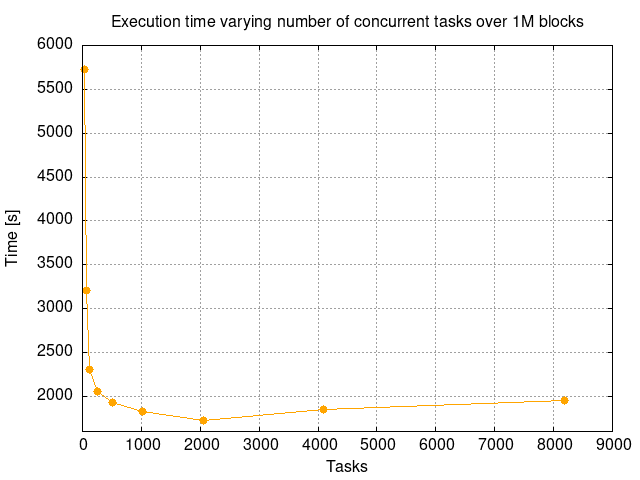
\includegraphics[width=0.8\textwidth]{Figures/results/num-tasks.png}
    \caption{Extraction time varying the number of concurrent tasks.}
    \label{fig:num-tasks}
\end{figure}

Eth2dgraph can be run with a variable amount of concurrent tasks that perform data extraction. This value can be set with the {\tt --num-tasks} option. Having too many concurrent tasks can overload the system where eth2dgraph or Ethereum node run. On the other hand, having just a few tasks makes the extraction process very slow. The best is to find the best balance point.
To find a good value for the number of tasks, I ran eth2dgraph with different amounts of tasks over one million blocks, from 10M to 11M. \cref{fig:num-tasks} shows the results of this test. As observed from the data, the optimal number of tasks for the machine used is around 2048, which is eight times the amount of available threads.

\section{Extraction of data}

\subsection{Extraction and Transformation}

To perform the extraction and transformation of Ethereum data to Dgraph format, eth2dgraph was run with the command reported in \cref{lst:extract-command}. The extraction was performed from block $0$ to block $17,265,420$, using $2048$ concurrent tasks. 

\begin{lstlisting}[language=Bash,caption={Eth2dgraph extraction command used.},label={lst:extract-command},captionpos=b,numbers=none]
eth2dgraph extract \
    -o extraction_output \
    -f 0 \
    -t 17265420 \
    --num-tasks 2048 \
    --include-tx \
    --include-transfers \
    --include-logs \
    -s smart-contract-sanctuary-ethereum/ \
    --size-output 100000 > eth2dgraph_extraction.logs & disown
\end{lstlisting}

\cref{table:extraction-stats} reports general statistics about the extraction process. The detailed sizes of the output folders are reported in \cref{table:extraction-output}.

\cref{fig:ram-usage-extraction} and \cref{fig:cpu-usage-extraction} shows respectively the RAM and CPU usage of the server during the process of data extraction. Data was obtained using the command~{\tt top -bn1 | awk '/Cpu/ \{ print \$2 \}' }~for the CPU and~{\tt free -m | awk '/Mem/\{print \$3\}' }~for the memory.
  

\begin{table}[H]
\centering
    \begin{threeparttable}
    \begin{tabular}{ m{5cm} m{3cm} } 
    \toprule
    \textbf{Parameter} & \textbf{Value}\\
    \midrule
    Total time   & 7h 15m 21s   \\ [1.2ex]
    Block/s      & 660.97       \\ [1.2ex]
    Contracts    & 60,016,663   \\ [1.2ex]
    Contract/s   & 2,297.6       \\ [1.2ex]
    Decompiler failures & 508,990 \\ [1.2ex]
    Output size  & 957 GiB        \\ [1.2ex]
    \bottomrule
    \end{tabular}
    \end{threeparttable}
    \caption{Statistics about extraction and transformation process.}
    \label{table:extraction-stats}
\end{table}

\begin{table}[H]
\centering
    \begin{threeparttable}
    \begin{tabular}{ m{5cm} m{3cm} } 
    \toprule
    \textbf{Folder} & \textbf{Size}\\
    \midrule
    {\tt / } & 957GiB \\
    {\tt /dynamic }    & 934GiB \\
    {\tt /static }     & 24GiB  \\
    & \\
    {\tt /static/blocks } & 1.2GiB  \\
    {\tt /static/events } & 548KiB    \\
    {\tt /static/destructions } & 3.4GiB    \\
    {\tt /static/deployments } & 18GiB  \\    
    {\tt /static/skeletons } & 903MiB    \\
    {\tt /static/errors } & 36KiB     \\
    {\tt /static/functions } & 8.5MB  \\  
    & \\
    {\tt /dynamic/transfers } & 129GiB    \\
    {\tt /dynamic/logs } & 263GiB    \\
    {\tt /dynamic/transactions } & 543GiB    \\
    \bottomrule
    \end{tabular}
    \end{threeparttable}
    \caption{Size of extracted data divided by folders.}
    \label{table:extraction-output}
\end{table}

\begin{figure}[H]
    \centering
    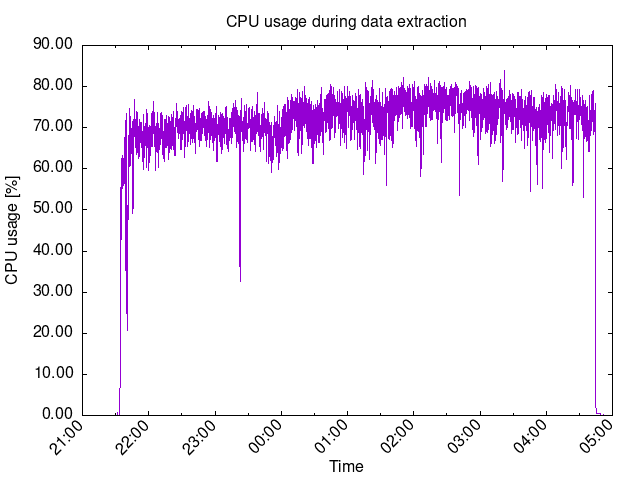
\includegraphics[width=0.9\textwidth]{Figures/results/cpu-usage-extraction.png}
    \caption{CPU usage of the server during data extraction.}
    \label{fig:cpu-usage-extraction}
\end{figure}

\begin{figure}[H]
    \centering
    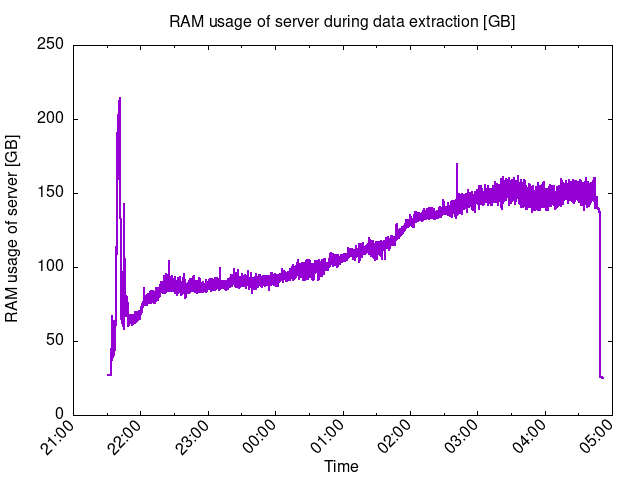
\includegraphics[width=0.9\textwidth]{Figures/results/ram-usage-extraction.png}
    \caption{Memory used by the server during data extraction}
    \label{fig:ram-usage-extraction}
\end{figure}

\subsection{Import in Dgraph}

Data was imported in Dgraph using the Bulk Loader. I faced a problem during the import of the complete dataset, the loader kept crashing. Analyzing the logs, it seemed that the crash was due to a hard limit on the size of local buffers. Removing this hard-coded limit allowed me to complete the import of data. I also submitted this fix\footnote{Pull Request can be seen here: \url{https://github.com/dgraph-io/dgraph/pull/8841}} in the open-source codebase of Dgraph. It was accepted, merged in the main branch and later included in the 23.0.1 release.

To perform the bulk import, I first ran with \cref{lst:zero-command} an instance of {\tt zero}, the Dgraph's node responsible of coordinating the distributed cluster. With the {\tt zero} running, the bulk import process was started with the command reported in \cref{lst:bulk-command}.

\begin{lstlisting}[language=Bash,caption={Command used for running {\tt zero}.},label={lst:zero-command},captionpos=b,numbers=none]
    dgraph zero --my=localhost:5080
\end{lstlisting}

\begin{lstlisting}[language=Bash,caption={Command used for running {\tt bulk loader}.},label={lst:bulk-command},captionpos=b,numbers=none]
dgraph bulk -f "<data-location>" \
	-s "<dql-schema-location>" \
	-g "<graphql-schema-location>" \
	--out "./out" \
	--map_shards=4 \
	--reduce_shards=1 \
	--zero=localhost:5080 \
	--mapoutput_mb=4096 \
	--num_go_routines=64 \
  --cleanup_tmp=false
\end{lstlisting}

The import of the complete dataset took 52 hours. Divided into 28 hours for the MAP phase and 24 hours for the REDUCE phase. It resulted in being the bottleneck of the process, it took around 7.5 times the amount of time needed for extracting the data. 

For memory heavy operations, Dgraph does not rely on the Go garbage collector, it uses \textit{jemalloc} to manually allocate memory. \cref{fig:import-ram-usage,fig:import-cpu-usage} show the RAM allocated by Dgraph during the phases of MAP and REDUCE of the bulk import. At least 400GiB of RAM are needed. Both steps have shown a big spike in memory allocation at around half of the process. The reasons of these spikes are not clear.

\begin{figure}[H]
    \centering
    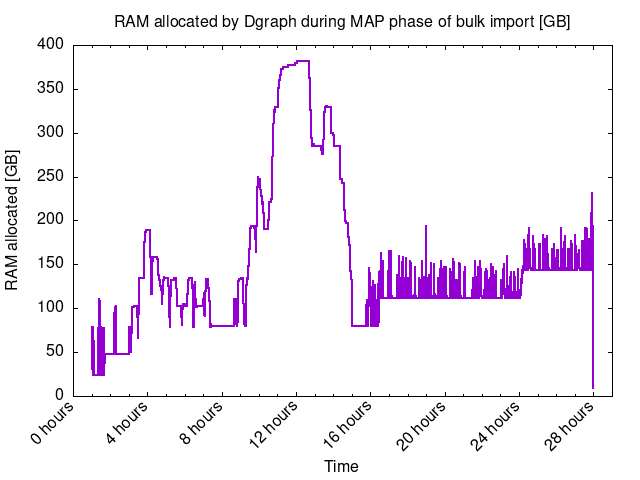
\includegraphics[width=0.9\textwidth]{Figures/results/MAP_RAM.png}
    \caption{RAM allocated by Dgraph with jemalloc during the MAP phase of the bulk import.}
    \label{fig:import-ram-usage}
\end{figure}

\begin{figure}[H]
    \centering
    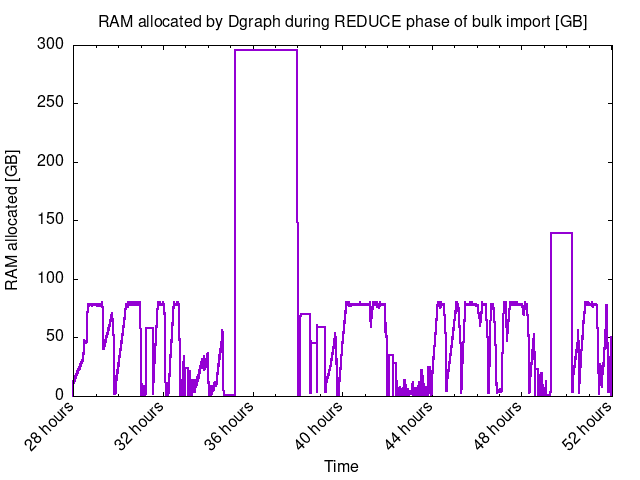
\includegraphics[width=0.9\textwidth]{Figures/results/REDUCE_RAM.png}
    \caption{RAM allocated by Dgraph with jemalloc during the REDUCE phase of the bulk import.}
    \label{fig:import-cpu-usage}
\end{figure}

The result of the bulk import is a folder called~{\tt p}~that contains the actual data in Dgraph's binary format. The size of this folder was of 2.5 TiB. 

From this folder, {\tt alpha}, the node responsible for managing the actual data, was run with the command shown in \cref{lst:alpha-command}. All the process was done with a locally-compiled version of Dgraph, but it is possible to perform the same steps using Docker. The details of the imported data, divided by types, are reported in \cref{table:imported-data-sizes}.

In contrast to importing the entire dataset, the import of the static data alone was completed in 1 hour, with an output of 112 GiB. This smaller dataset statically describes all the smart contracts of the Ethereum blockchain, without information on their usage. 

\begin{lstlisting}[language=Bash,caption={Command used for running the {\tt alpha} instance.},label={lst:alpha-command},captionpos=b,numbers=none]
dgraph alpha 
    --my=localhost:7080 \
    --zero=localhost:5080 \
    --security whitelist=0.0.0.0/0 \
    --cache "size-mb=20000; percentage=50,30,20;" \
    --badger="compression=snappy; numgoroutines=64;"
\end{lstlisting}

\begin{table}[H]
\centering
    \begin{threeparttable}
    \begin{tabular}{ m{3.8cm} m{3cm} m{2cm} m{4cm} } 
    \toprule
    \textbf{Type} & \textbf{Entries} & \textbf{Disk size} & \textbf{Uncompressed size} \\
    \midrule
    Transaction   & 1,967,716,025 & 1.3TiB & 2.8TiB \\ [1.2ex]
    Log   & 2,795,971,346 & 823.6GiB & 2.2TiB \\ [1.2ex]
    TokenTransfer   & 1,437,470,051 & 181.1GiB & 414.0GiB \\ [1.2ex]
    ContractDeployment   & 60,016,663 & 82.0GiB & 161.3GiB \\ [1.2ex]
    Account   & 286,391,265 & 29.7GiB & 52.2GiB \\ [1.2ex]
    ContractDestruction   & 55,152,100 & 9.7GiB & 22.5GiB \\ [1.2ex]
    Block   & 17,265,421 & 5.7GiB & 16.7GiB \\ [1.2ex]
    Skeleton   & 467,318 & 1.5GiB & 7.0GiB \\ [1.2ex]
    Withdrawal   & 3,688,662 & 285.7MiB & 956.5MiB \\ [1.2ex]
    Function   & 139,603 & 42.1MiB & 84.9MiB \\ [1.2ex]
    Event   & 9,690 & 2.1MiB & 4.0MiB \\ [1.2ex]
    Error   & 545 & 118.5KiB & 228.6KiB \\ [1.2ex]
    \bottomrule
    \end{tabular}
    \end{threeparttable}
    \caption{Cardinalities and sizes of entries stored in Dgraph\protect\footnotemark.}
    \label{table:imported-data-sizes}
\end{table}
\footnotetext{Data about sizes was obtained querying the {\tt /state} endpoint of the {\tt alpha} instance.}

 \section{Querying data}

Dgraph exposes two endpoints for querying the data: one for DQL at \\{\tt /query} and one for GraphQL at {\tt /graphql}.

DQL is the query language built by the Dgraph team to query and mutate data in this database. It has powerful features such as query variables, math on attributes, recursive queries and shortest path search. Under the hood, every GraphQL query is translated to DQL before being executed, so everything that can be done with GraphQL can be done with DQL, but not the opposite.

To easily perform DQL queries, Dgraph provides a web application called \textit{Ratel}\footnote{Ratel is a web application for querying, visualizing and managing Dgraph's data: \url{https://github.com/dgraph-io/ratel}}. It gives a friendly user interface to get and visualize query results. \Cref{fig:ratel-1} shows an example of query in which it is visualized the ABI of a contract. \Cref{fig:ratel-2} shows accounts linked by transactions.

\begin{figure}[H]
    \centering
    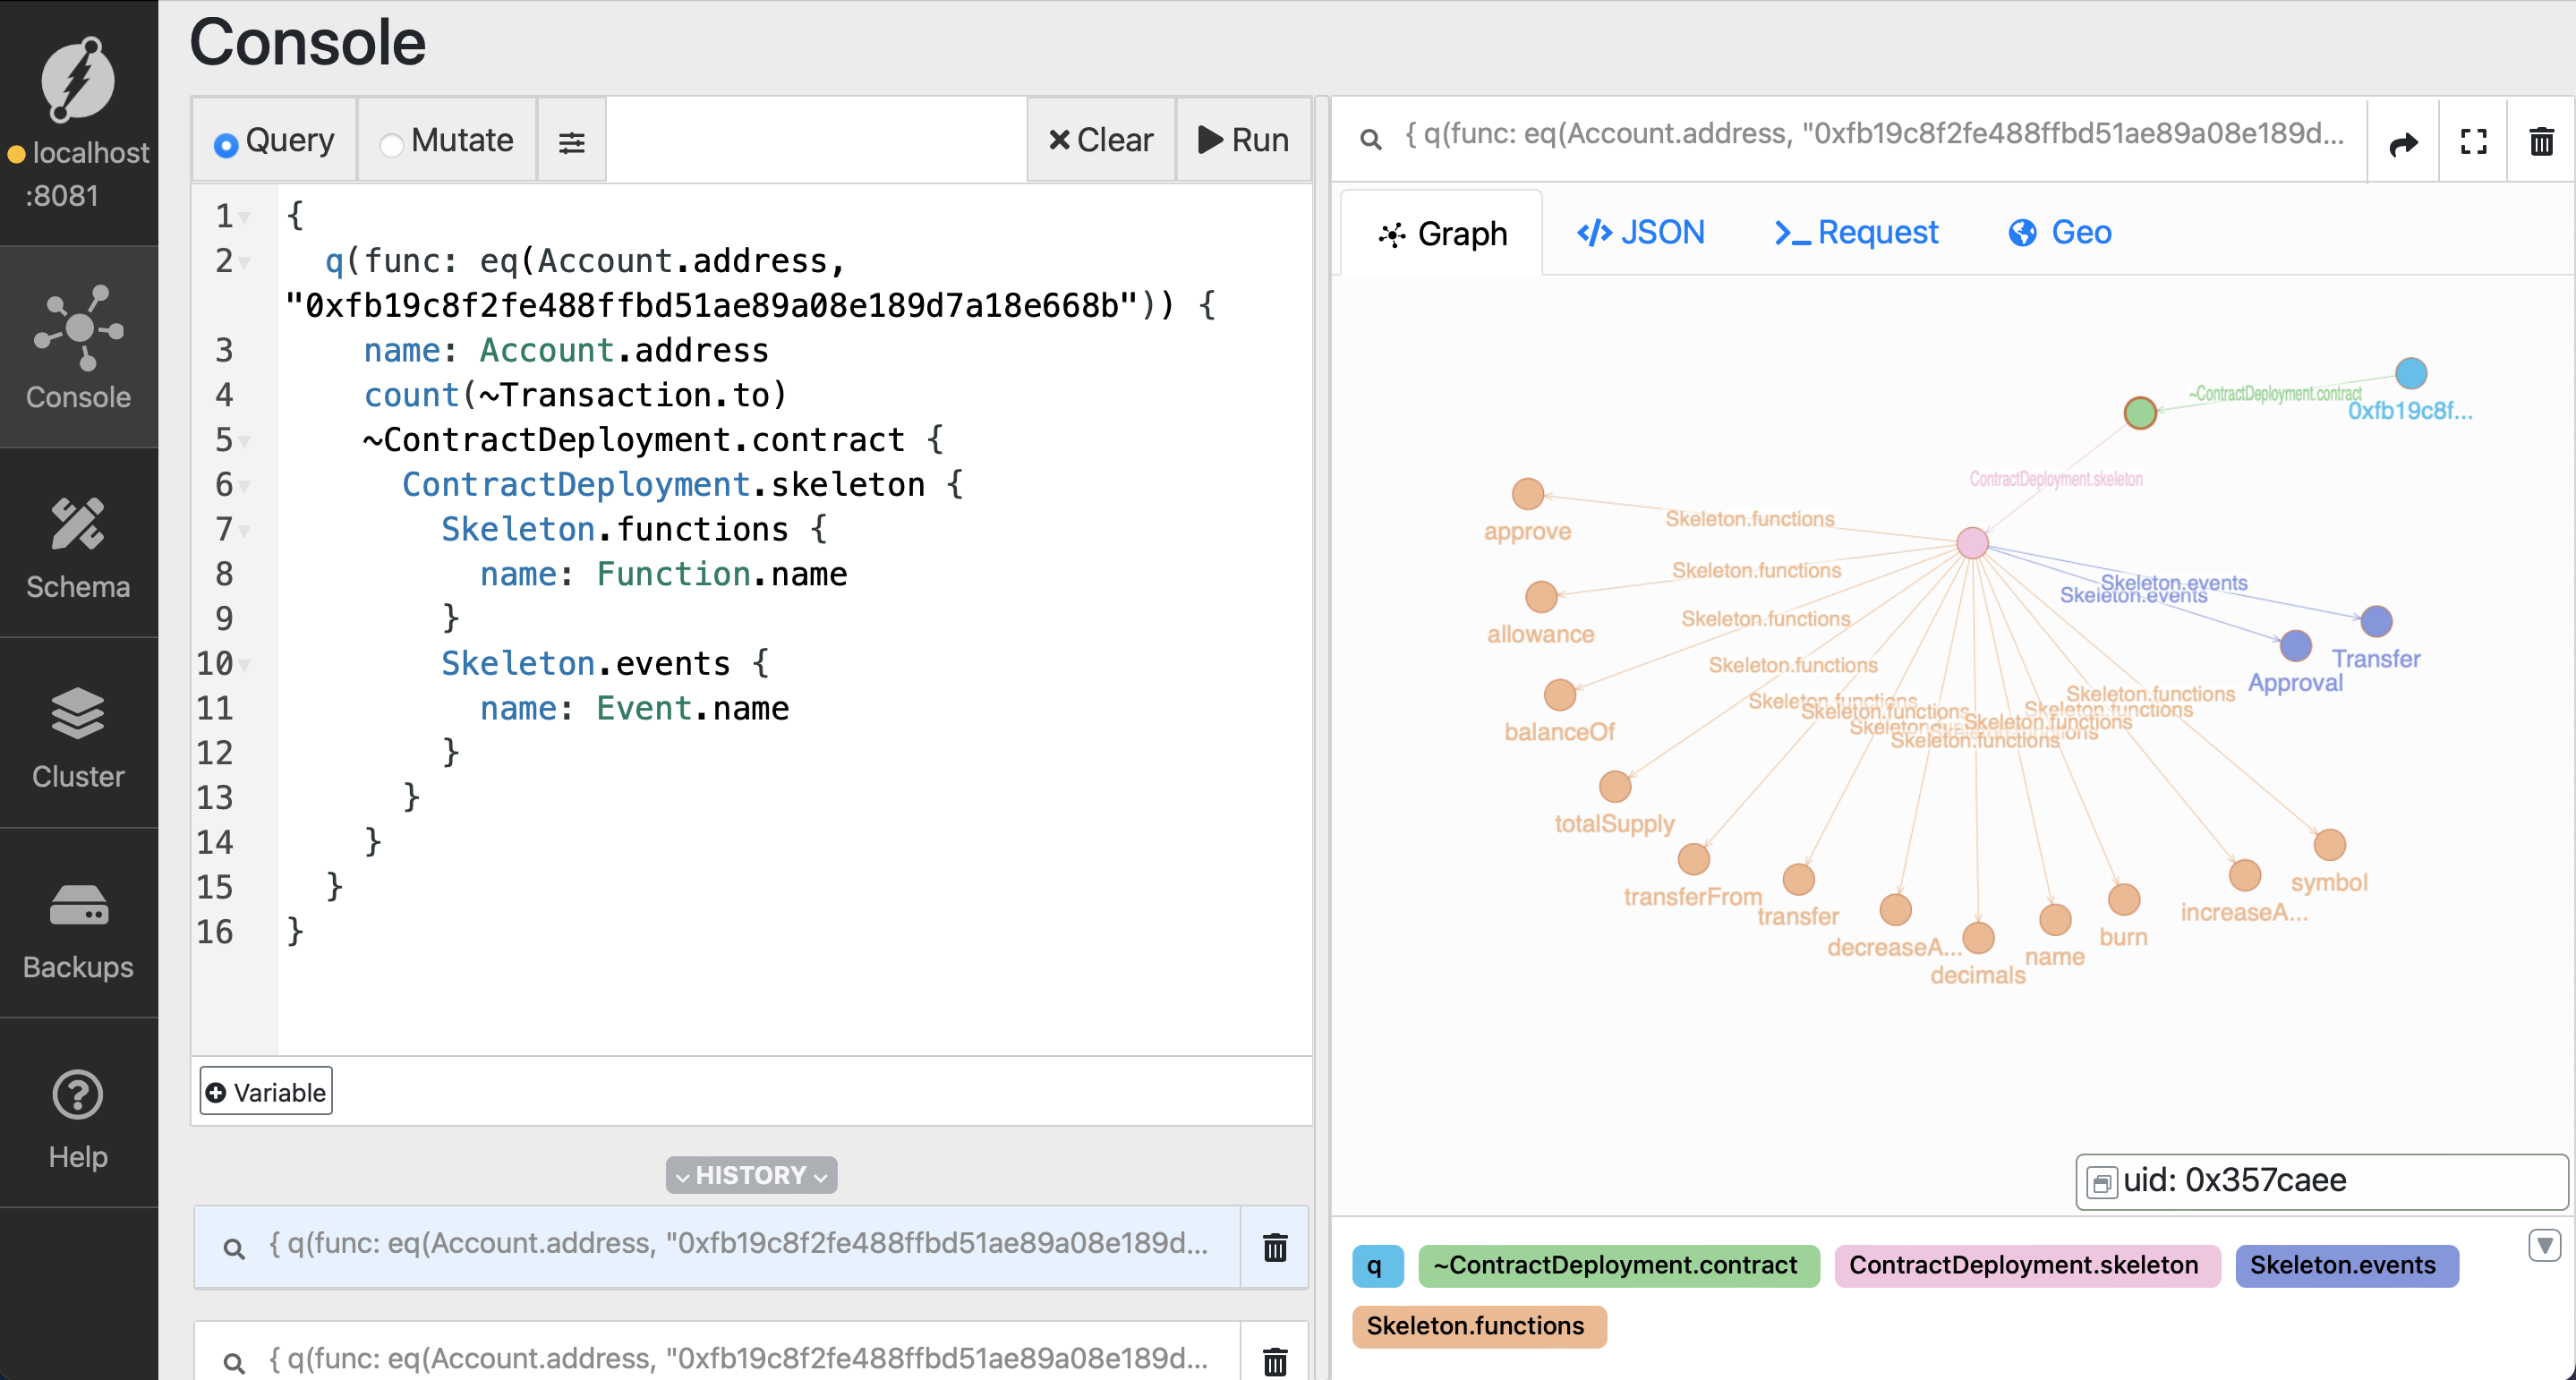
\includegraphics[width=1\textwidth]{Figures/results/ratel-1.png}
    \caption{Visualization of Contract's ABI in Ratel.}
    \label{fig:ratel-1}
\end{figure}

\begin{figure}[H]
    \centering
    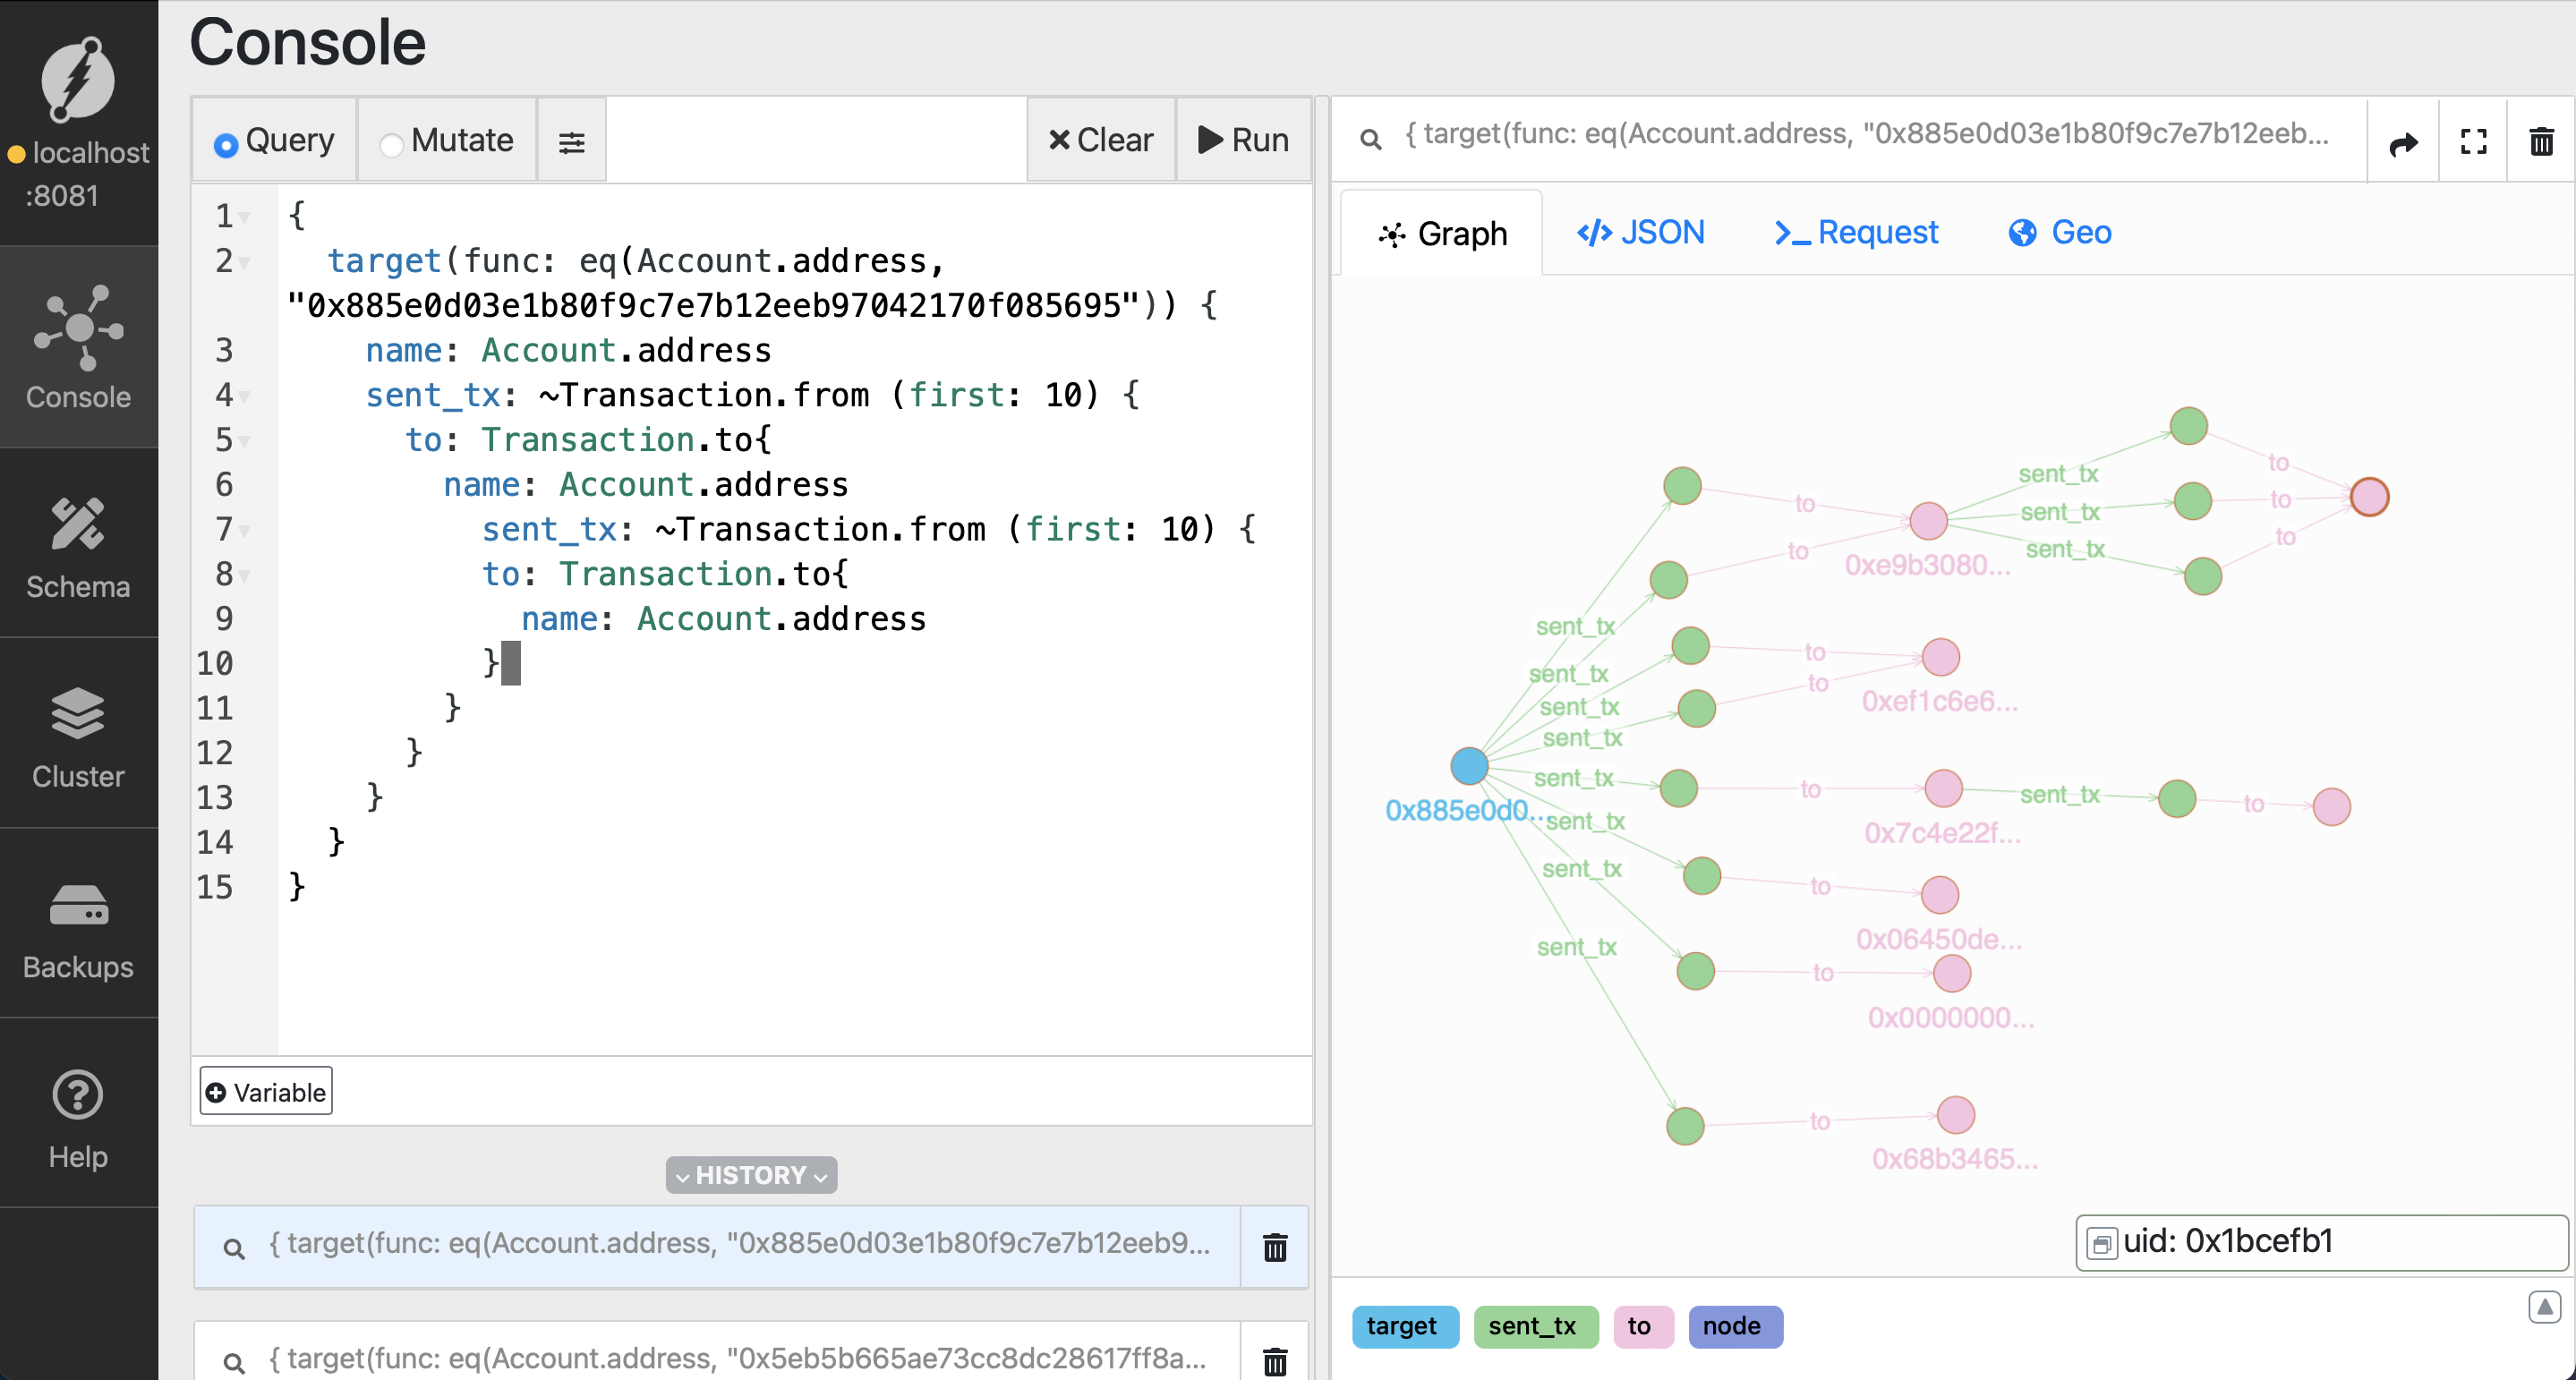
\includegraphics[width=1\textwidth]{Figures/results/ratel-2.png}
    \caption{Visualization of Accounts linked by Transactions in Ratel.}
    \label{fig:ratel-2}
\end{figure}

\subsection{Query performance}

In this section, I provide examples of queries with their corresponding execution times. The processing time mentioned in table \cref{table:queries-results} is included by the database in the query responses. It does not include decoding, encoding or network transfers, just the time needed by Dgraph to get the data.

\begin{lstlisting}[caption={Query to get all the transactions sent by a specific address. Response included 1071 transactions.},label={lst:query-1},captionpos=b,numbers=none]
{
    q(func: eq(Account.address, "0xd8da6bf26964af9d7eed9e03e53415d37aa96045")){
        ~Transaction.from{
            expand(_all_)
        }
    }
}
\end{lstlisting}

\begin{lstlisting}[caption={Query to get all the transfers of BoredApe NFT with id \textit{1020} (686 transfers).},label={lst:query-2},captionpos=b,numbers=none]
{
    BOREDAPE as var(func: eq(Account.address, "0xbc4ca0eda7647a8ab7c2061c2e118a18a936f13d"))
	q(func: uid(BOREDAPE)) {
        transfers: ~TokenTransfer.contract @filter(eq(TokenTransfer.token_id, "1020" )) {
            TokenTransfer.block {
                Block.number
                Block.datetime
            }
            TokenTransfer.from {
                Account.address
            }
            TokenTransfer.to {
                Account.address
            }
        }
	}
}
\end{lstlisting}

\begin{lstlisting}[caption={Query to count all the transactions in the database.},label={lst:query-3},captionpos=b,numbers=none]
{
    var(func: type(Transaction)) {
        countVar as count(uid)
    }
    agg() {
        count: max(val(countVar))
    }
}
\end{lstlisting}

\begin{lstlisting}[caption={Query to get the addresses of contracts that implement a function with name \textit{trade} (554 addresses).},label={lst:query-4},captionpos=b,numbers=none]
{
    q(func: eq(Function.name, "trade")) @normalize {
        ~Skeleton.functions {
            ~ContractDeployment.skeleton {
                ContractDeployment.contract {
                    address: Account.address
                }
            }
        }
    }
}
\end{lstlisting}

\begin{lstlisting}[caption={Query to compute the ETH burnt after London upgrade.},label={lst:query-5},captionpos=b,numbers=none]
{
    var(func: ge(Block.number, 12965000))  {
        price as Block.base_fee_per_gas
        used as Block.gas_used
        gasBurnt as math(price * used)
    }
    q() {
        totBurnt as sum(val(gasBurnt))
        ethBurnt as math(totBurnt / 1000000000)
        usdBurnt: math(ethBurnt * 1870) 
    }
}
\end{lstlisting}

\begin{table}[H]
\centering
    \begin{threeparttable}
    \begin{tabular}{ m{3cm} m{5cm} } 
    \toprule
    \textbf{Query} & \textbf{Processing time [ms]}\\
    \midrule
    \cref{lst:query-1}   & 1671.46  \\ [1.2ex]
    \cref{lst:query-2}   & 416.70  \\ [1.2ex]
    \cref{lst:query-3}   & 73881.76  \\ [1.2ex]
    \cref{lst:query-4}   & 165.65  \\ [1.2ex]
    \cref{lst:query-5}   & 31868.36  \\ [1.2ex]
    \bottomrule
    \end{tabular}
    \end{threeparttable}
    \caption{Processing time of DQL queries. }
    \label{table:queries-results}
\end{table}
 
\section{Comparison with Ethereum-ETL}

Eth2dgraph was compared against Ethereum-ETL, one of the most popular open-source tools to export Ethereum data. The two tools serve the same purpose: extract and transform Ethereum data to be more usable.
Ethereum-ETL does so by exporting data to CSV files, that can eventually be loaded into relational databases, while eth2dgraph does so by exporting data to compressed JSON files that can be imported into Dgraph. 

At a high level, the two tools work in a similar way. They both fetch data using the Ethereum RPC interface. They both can be used through a CLI.

Ethereum-ETL does not integrate a decompiler to get the ABI of the smart contracts. It simply stores the raw four bytes of the function selectors that can be found as arguments of the {\tt PUSH4} opcode at the beginning of the contracts' bytecodes. 

Another design difference is in the steps needed to get the data. Ethereum-ETL needs multiple extraction steps to get certain kinds of information. For example, to get smart contracts data, it first needs to get and store the list of contracts' addresses, then, for each address, it fetches the contract's data. Eth2dgraph does everything in a single extraction step using the traces, to make the process faster.

The comparison was made by extracting data on various block ranges. There are multiple ways of using Ethereum-ETL. For this comparison, it was run with the command {\tt export\_all}. This command produces a similar output to the one of eth2dgraph, with the difference that it includes transaction receipts but it does not use the traces. The usage of receipts instead of traces means that all the contracts created by other contracts are not included in the output data. 

\Cref{lst:ethereum-etl-command,lst:eth2dgraph-command} shows the commands used to run the tools for the comparison. Both tools were run on the same machine and using the same Ethereum node. For the run on 400k blocks, Ethereum-ETL was run with batch size\footnote{The batch size indicates how many calls are sent together to the Ethereum node.} reduced to 20. This was done since the default size of 100 caused the program to crash. The results are reported in \cref{table:tools-comparison-2}. 

\begin{lstlisting}[caption={Command for running Ethereum-ETL in the comparison},label={lst:ethereum-etl-command},captionpos=b,numbers=none]
ethereumetl export_all \
    -s <from> \
    -e <to> \
    -p http://localhost:8545 \
    -o <output-folder> \
    -w 2048
\end{lstlisting}

\begin{lstlisting}[caption={Command for running eth2dgraph in the comparison},label={lst:eth2dgraph-command},captionpos=b,numbers=none]
eth2dgraph extract \
    -f <from> \
    -t <to> \
    --num-tasks 2048 \
    --include-tx \
    --include-logs \
    --include-transfers \
     -o <output-folder> 
\end{lstlisting}

\begin{table}[H]
\centering
    \begin{threeparttable}
    \begin{tabular}{ c c c c } 
    \toprule
    \textbf{Blocks range} & \textbf{Ethereum-ETL} & \textbf{eth2dgraph} & \textbf{Speedup} \\
    \midrule
    12000000-12001000   & 1m 57s & 8s & 14.6x \\ [1.2ex]  
    16000000-16010000   & 14m 18s & 53.48s & 16x \\ [1.2ex] 
    17000000-17100000   & 2h 56m 53s & 6m 45s & 26.2x \\ [1.2ex]   
    14000000-14400000   & 13h 30m 21s & 31m 10s & 48x \\ [1.2ex]
    \bottomrule
    \end{tabular}
    \end{threeparttable}
    \caption{Results of performance comparison between Ethereum-ETL and eth2dgraph. }
    \label{table:tools-comparison-2}
\end{table}

Overall, eth2dgraph was at least one order of magnitude faster than Ethereum-ETL in all the extractions performed. This shows the effectiveness of the design choices taken while developing eth2dgraph. With growing block ranges, eth2dgraph becomes faster because the caching logic allows it to avoid decompiling contracts.


\cleardoublepage


\chapter{Analysis of data}
\label{chapter-analysis}

In this chapter, I analyse the data that have been extracted by {\tt eth2dgraph}. Each section describes an independent analysis.

All the results refer to data from block $0$ to block $17,265,420$ of the Ethereum {\tt mainnet}. It corresponds to the period of time between July 30 2015 to May 15 2023 (7 years, 9 months, and 15 days).

\section{General data overview}

This analysis is conducted to give a general overview of the data extracted. There are some interesting analysis results that help to understand the current state of the Ethereum chain. Here are some interesting points:

\begin{itemize}
    \item 60,016,663 smart contract deployments, of which 213,406 failed, were found with 59,429,189 unique addresses. 88\% of them (52,343,783) never emitted logs. 87\% of them (51,974,197) never received a single transaction. Just 5.78\% (3,435,332) of contracts' addresses both received at least one transaction and emitted at least one log. This shows that the vast majority of the deployed smart contracts are never actively used. \Cref{fig:contracts-by-usage} shows the distribution of smart contracts based on their active usage.
    
    \item There are 2.8B logs emitted. 10 smart contracts alone, reported in \cref{table:top-logs-emitters}, emitted the 24.25\% of all logs. Top 100 contracts emitted 38.83\% of the logs. Top 1,000 contracts emitted 57.53\% of the logs. 33,287 smart contracts (0.056\% of the total) emitted 90\% of the logs. Most of the activity on the chain is restricted to a relatively small group of smart contracts.
    
    \item Transactions are more evenly distributed compared to logs. There are 165,684,328 distinct EOAs that have sent transactions. Top 10 senders sent 6.96\% of all transactions. 90\% of transactions were sent by top 25\% addresses. 
    
    \item There are 286,391,265 distinct addresses that have received transactions. The top 10 receivers received 18.55\% of all the transactions, and there is just one receiver in the top 10 that is not a contract\footnote{It is an address of the Coinbase exchange {\tt 0xa090e606e30bd747d4e6245a1517ebe430f0057e}.}. 90\% of transactions were received by the top 57.85\% receivers.
    
    \item 61.92\% of transactions are sent to smart contracts. 0.25\% are sent to the null address {\tt 0x0}. The remaining 37.83\% are transactions from EOAs to other EOAs or unclaimed addresses.
    
    \item \cref{fig:deploy-history} shows the history of smart contracts deployments. The growth in deployments was exponential until the beginning of 2018. After an initial period in which there were more deployments done by users than by contracts, now the majority of smart contracts are deployed using the CREATE or CREATE2 opcodes. This confirms the trend observed by Kiffer et al.~\cite{ethereum-sc-topology}. They observed this phenomenon in data until 2018. The difference in deployments by users or by contracts has grown since then. Since 2019, the difference has been of at least one order of magnitude.
\end{itemize}

\begin{figure}[!ht]
    \centering
    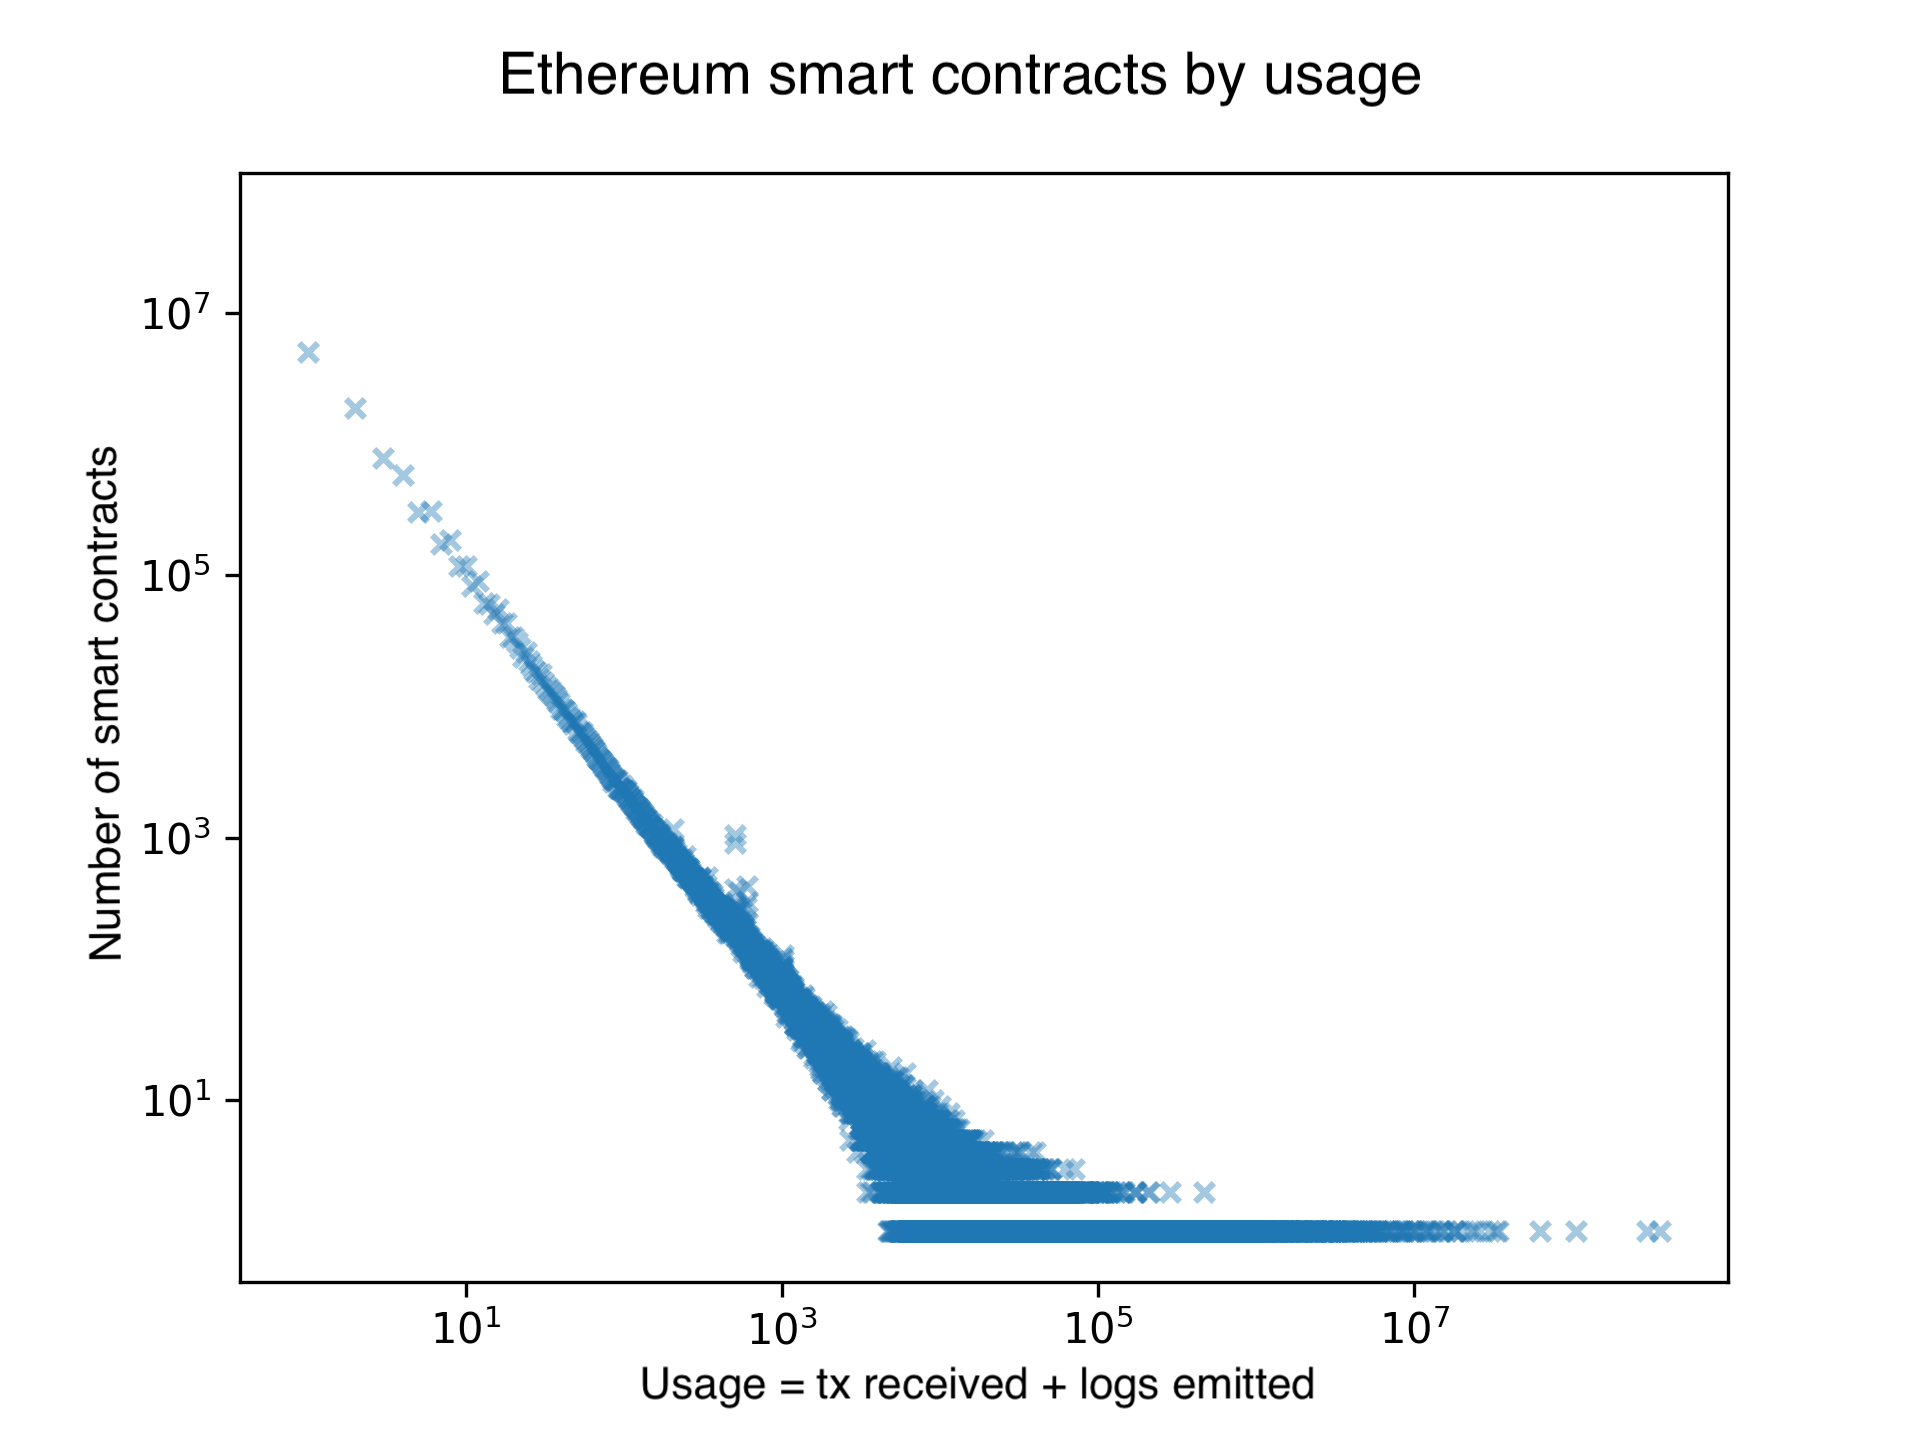
\includegraphics[width=1\textwidth]{Figures/analysis/contracts_by_usage.png}
    \caption{Ethereum smart contracts by usage, note the log scale on both axes.}
    \label{fig:contracts-by-usage}
\end{figure}

\begin{table}[!ht]
\centering
    \begin{threeparttable}
    \begin{tabular}{ c c c } 
    \toprule
    \textbf{Name of contract} & \textbf{Contract address} & \textbf{Logs emitted} \\
    \midrule
       Wrapped Ether & \small{0xc02aaa39b223fe8d0a0e5c4f27ead9083c756cc2} & 282,095,104  \\ [1.2ex]
       Tether USD  & \small{0xdac17f958d2ee523a2206206994597c13d831ec7} & 196,788,993  \\ [1.2ex]
       USD Coin & \small{0xa0b86991c6218b36c1d19d4a2e9eb0ce3606eb48} & 74,321,927  \\ [1.2ex]
       XEN & \small{0x06450dee7fd2fb8e39061434babcfc05599a6fb8} & 30,438,737  \\ [1.2ex]
       DAI Stablecoin& \small{0x6b175474e89094c44da98b954eedeac495271d0f} & 20,283,129  \\ [1.2ex]
       Seaport & \small{0x00000000006c3852cbef3e08e8df289169ede581} & 16,764,010  \\ [1.2ex]
       ChainLink Token & \small{0x514910771af9ca656af840dff83e8264ecf986ca} & 16,698,857  \\ [1.2ex]
       Wyvern Exchange & \small{0x7be8076f4ea4a4ad08075c2508e481d6c946d12b} & 15,735,740  \\ [1.2ex]
       SHIBA INU & \small{0x95ad61b0a150d79219dcf64e1e6cc01f0b64c4ce} & 12,607,046  \\ [1.2ex]
       Forsage & \small{0x5acc84a3e955bdd76467d3348077d003f00ffb97} & 12,323,018  \\ [1.2ex]  
    \bottomrule
    \end{tabular}
    \end{threeparttable}
    \caption{Top 10 smart contracts per logs emitted.}
    \label{table:top-logs-emitters}
\end{table}

\begin{figure}[!ht]
    \centering
    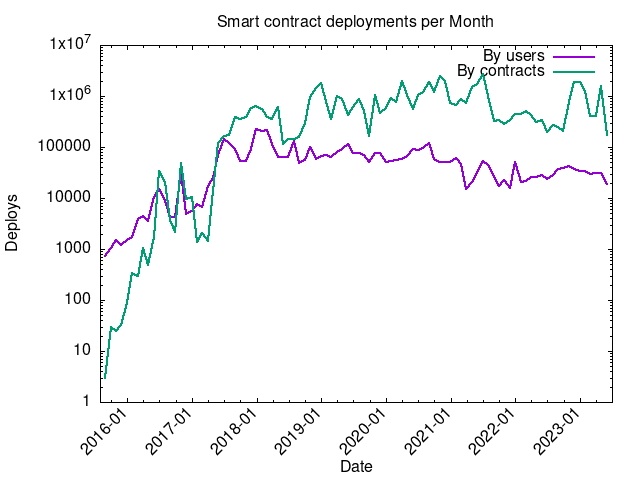
\includegraphics[width=1\textwidth]{Figures/analysis/deploys_per_month.png}
    \caption{Smart contract deployments over time grouped by month.}
    \label{fig:deploy-history}
\end{figure}

\newpage

\section{Skeleton clusters}

The skeleton of a smart contract is its deployed bytecode without the arguments of the PUSH opcodes and the eventual metadata appended at the end. \Cref{skeleton-section} describes this concept and explains how eth2dgraph extracts the skeletons from the Ethereum chain.

Out of the 60M smart contracts deployments in the history of Ethereum, just 467K distinct skeletons were found. This allows us to link smart contracts with each other based on skeleton equality. On average, each smart contract has 128 semantically identical siblings. 

The distribution of smart contracts by skeleton is not uniform. There are 361,546 skeletons (77.4\%) that correspond to a single deployed Ethereum smart contract. At the same time, there are skeletons that correspond to millions of smart contract deployments. The most frequently used skeleton matched 12.2M deployments and was related to gas tokens, as shown in \cref{most-deployed-skeletons}.

\subsection{Most deployed skeletons}
\label{most-deployed-skeletons}

I analyze the top 10 skeletons found on the Ethereum chain by a number of deployments. These 10 distinct skeletons correspond together to 44,389,576 smart contract deployments (73.96\% of the total).

\begin{itemize}

    \item The most used skeleton is related to gas reserves. It is the way gas tokens store gas when it is bought. The concept of the gas token is analyzed in \cref{gas-tokens}. This skeleton has a very simple bytecode that just allows a particular address, with a length of 14 bytes, to destroy the contract. The size of this skeleton is 21 bytes. It has been deployed 12,240,689 times.
    
    \item The second skeleton is the implementation of the ERC-1167\footnote{Specification of the ERC-1167 Minimal Proxy Contract: \url{https://eips.ethereum.org/EIPS/eip-1167}} logic. This bytecode consists of a minimal proxy that forwards all the calls it receives to a fixed hard-coded address. The size of this skeleton is of 45 bytes. It has been used 11,168,872 times.

    \item The third skeleton is again related to gas tokens. It is the same logic as the first described skeleton but with the allowed address of 15 bytes instead of 14. It has been used 6,829,142 times. Its size is 22 bytes.

    \item The fourth skeleton is simply the empty bytecode. It is valid in the Ethereum protocol to have empty smart contracts. 4,877,139 deployments with no bytecode were found.

    \item The fifth skeleton is again related to gas tokens. It is the same logic as the previous two but with the length of the allowed address of 20 bytes. 2,138,723 deployments matching this skeleton were found with a size of 27 bytes.

    \item The sixth skeleton represents 1,665,668 user wallets of the \textit{Bittrex} exchange\footnote{Bittrex is a crypto exchange platform: \url{https://global.bittrex.com/}.}. Each of these smart contracts is a controlled wallet. This means that each contract represents a user of the exchange, but the control over the Ethers and tokens remains under the company. The point of having these controlled wallets is to give users a unique address to send their tokens or Ethers. The size of this skeleton is of 502 bytes.

    \item The seventh skeleton has been used 1,549,146 times and represents an \textit{OwnableDelegateProxy}. It is a proxy contract, so it simply forwards the received calls to another contract that implements the actual logic, using {\tt delegatecall}. This specific type of proxy has two additional properties:
    \begin{itemize}
        \item \textit{Ownable}: it stores the address of the owner and allows it to modify the implementation address. The ownership can eventually be transferred.
        \item \textit{Upgradable}: it is possible to update the address of the implementation, changing where the proxy is forwarding the calls.
    \end{itemize}
    All the previous logic is implemented in a bytecode with a size of 1073 bytes.

    \item The eighth skeleton has been used 1,542,310 times and represents a \textit{forwarder contract}. This skeleton has two main public functions: \textit{flush()} and \textit{flushTokens(address)}. They are used to transfer ETH and tokens to a fixed parent address. The point of this kind of contract is to have multiple receive addresses for the same wallet. ETH transfers are automatically sent to the parent address, while tokens can be flushed with a transaction. Bitgo\footnote{Bitgo is a digital asset trust company: \url{https://www.bitgo.com/}} uses this contract in their implementation of the multi-signature wallet\footnote{Source code of the multi-signature wallet: \url{https://github.com/BitGo/eth-multisig-v2/tree/master}}. The size of this skeleton is of 785 bytes.

    \item The ninth skeleton is a proxy used for the Ambi Multisig wallet as found by di Angelo and Salzer~\cite{wallet-contracts}. It has been deployed 1,202,291, with a size of 88 bytes. 

    \item The tenth skeleton has been used 1,175,596 times and it is the exact same forwarding logic of the eighth skeleton. The few small differences are probably due to the compiler version or optimization level. Its size is 789 bytes.
    
\end{itemize}

I calculated cosine and interface similarity of the top 10 skeletons to find similarities between them and all the other skeletons. This formed seven clusters shown in \cref{table:top-skeletons-clusters}.

These 7 clusters describe 75.29\% of all the deployments that happened in the Ethereum blockchain. They can be grouped in just 4 distinct categories: \textit{gas token}, \textit{proxy}, \textit{wallet} and \textit{empty contract}.

\begin{table}[H]
\centering
    \begin{threeparttable}
    \begin{tabular}{ c c c c } 
    \toprule
    \textbf{\# Group} & \textbf{Distinct skeletons} & \textbf{Deployments} & \textbf{Category} \\
    \midrule  
    1 & 5 & 21,787,384 & Gas token \\ [1.2ex]
    2 & 6 & 11,169,089 & Proxy \\ [1.2ex]
    3 & 1 & 4,877,139 & Empty contract \\ [1.2ex]
    4 & 31 & 2,732,644 & Wallet \\ [1.2ex]
    5 & 5 & 1,863,898 & Wallet \\ [1.2ex]
    6 & 20 & 1,55,2654 & Proxy \\ [1.2ex]
    7 & 3 & 1,202,787 & Wallet \\ [1.2ex]
    \bottomrule
    \end{tabular}
    \end{threeparttable}
    \caption{Clusters formed by grouping top 10 skeletons with their similars.}
    \label{table:top-skeletons-clusters}
\end{table}

\subsection{New skeletons over time}

An interesting metric to observe is when the skeletons were first seen on the blockchain. This is a different indicator to the one shown in \cref{fig:deploy-history}, since it just shows when semantically new smart contracts are deployed, avoiding all the replicas.

\Cref{fig:skeletons-deploy} shows, for each month, the number of new skeletons found on the Ethereum chain. While the number of monthly deployments has not increased since 2021, the number of new monthly skeletons has kept increasing. This is also visible in \cref{fig:skeletons-ratio}, especially in the year 2022 in which the ratio between deployments and new skeletons was low compared to the past. From this data, it appears that code reuse is dropping. 

\begin{figure}[H]
    \centering
    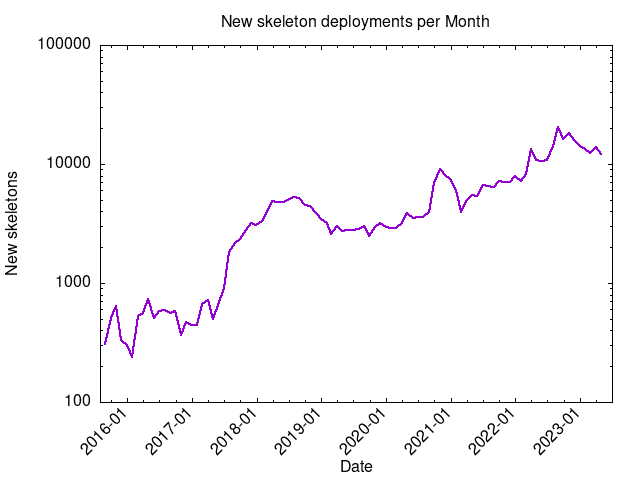
\includegraphics[width=0.9\textwidth]{Figures/analysis/skeletons_per_month.png}
    \caption{Deployments of new skeletons over time, grouped by month}
    \label{fig:skeletons-deploy}
\end{figure}

\begin{figure}[H]
    \centering
    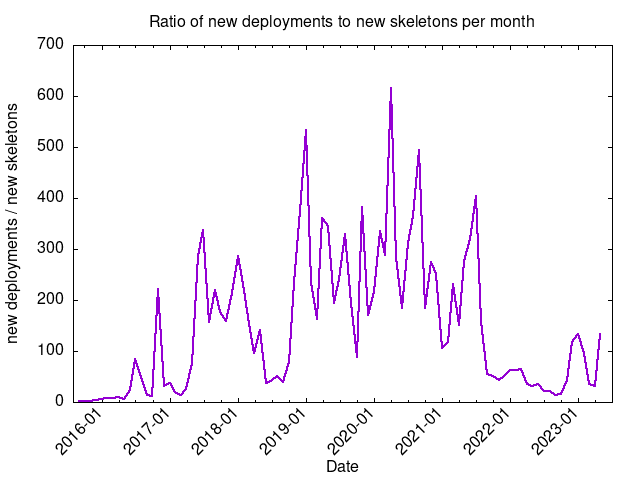
\includegraphics[width=0.9\textwidth]{Figures/analysis/ratio_per_month.png}
    \caption{Ratio of deployments to new skeletons over time, grouped by month. High values imply more duplicates deployed.}
    \label{fig:skeletons-ratio}
\end{figure}


\newpage

\section{Metamorphic contracts}

Smart Contracts are commonly thought to be immutable: once deployed on the Ethereum blockchain their code can not be changed. This was true until the introduction of the {\tt CREATE2} opcode in EIP-1014, included in the Constantinople Upgrade. This new opcode gives developers more control over the deployment address of the contracts created. 

With the {\tt CREATE} opcode, the new address is calculated as

\[a=keccak256(RLP(d,n_d))[12:] \]

in which $d$ denotes the \textit{deployer} address and $n_d$ the deployer \textit{nonce}. The nonce is updated by the protocol after every deployment. This prevents the possibility of deploying twice at the same address.

With {\tt CREATE2}, the newly created address is computed as

\[a=keccak256({\tt 0xff}\,||\,d\,||\,s\,||\,keccak256(c))[12:]\]

where {\tt 0xff} is a constant byte, $s$ is a salt picked by the deployer and c is the initialization code of the contract. The developer invoking {\tt CREATE2} has full control over all the variables, so it is easy to predict and manipulate the new address. The address to which the contract is deployed must be empty, this means that no contracts were ever deployed there or they were all previously destroyed.

With {\tt CREATE2} it is possible to deploy a smart contract to a certain address $a$, then destroy it and re-deploy it again with the same bytecode at the same address $a$. This event is called \textit{resurrection} by Fröwis and Böhme~\cite{create2-metamorphic}. 

Since the initialisation code of a contract can read the blockchain state, it is possible to use it in a way such that the same initialisation code, run multiple times, results in different deployed bytecodes. An easy way of doing so is by instructing it to ask for a third smart contract for the code to deploy. This third contract can change the code it gives back from time to time. This is one way of deploying different bytecodes at the same address, creating a \textit{metamorphic} smart contract. \cref{lst:meta-1,lst:meta-2} give an example of this pattern with pseudo code.

\begin{lstlisting}[label={lst:meta-1},caption={Pseudo initialization code that gets the code to deploy from another contract.}]
third_contract = address("0xab12...5134")
return third_contract.get_code()
\end{lstlisting}

\begin{lstlisting}[label={lst:meta-2},caption={Pseudo code of a contract that gives back the code to be deployed.}]
bytes code_to_deploy;

function setCode(bytes calldata _data) public {
    code_to_deploy = _data;
}
function getCode() public returns (bytes memory) {
    return code_to_deploy;
}
\end{lstlisting}

Another more complicated way to replace the deployed code of a contract is by combining {\tt CREATE} and {\tt CREATE2} together. {\tt CREATE2} is used to reset the nonce used in {\tt CREATE}. This can be done with the following steps:

\begin{enumerate}
    \item A deployer contract $D$ creates a \textit{factory} contract, here called $F$, at address $A_{f}$ using {\tt CREATE2}. $A_{f}$ is computed as $keccak256({\tt 0xff}\,||\,A_D\,||\,s\,||\,keccak256(c))[12:]$, in which $s$ is any random salt and $c$ is the initialization code of $F$.  

    \item Through $F$, a new contract $C_1$ is created using the {\tt CREATE} opcode at address $A_{c1}$. $A_{c1}$ will be calculated as $keccak256(RLP(A_f,n_d))[12:]$, in which $n_d$, the nonce, is zero.

    \item The factory $F$ is destroyed with {\tt SELFDESTRUCT} and redeployed again by $D$ at the same address $A_f$ and with the same code. This is achieved using {\tt CREATE2} with the same parameters. This step is needed to reset the nonce of $F$.

    \item The contract $C_1$ is destroyed with {\tt SELFDESTRUCT}.

    \item Now, $F$ can deploy a new contract with arbitrary code using {\tt CREATE}. The newly created contract will have the same address $A_{c1}$, since it is calculated as $keccak256(RLP(A_f,n_d))[12:]$ with $n_d$ equals to zero, as in step 2. 
    
\end{enumerate}

\subsection{Overview of metamorphic contracts usage}

Fröwis and Böhme~\cite{create2-metamorphic} analyzed metamorphic contracts until July 2021. They found 41 accounts that received deployments with different bytecodes. From a manual analysis, they concluded that this phenomena was used by just a few experienced users. They did not find any malicious use of this pattern. Most of the cases were about smart contracts related to the front-running infrastructure.

I here analyze the usage of this pattern in the data until May 15 2023, almost two years of data after the analysis conducted by Fröwis and Böhme.

A total of 267,461 accounts received multiple deployments of the \textbf{same} bytecode, these are the resurrected accounts. For the metamorphic pattern, there are 524 distinct accounts that have mutated bytecode over time. Out of these 524, 295 have probably used the pattern with just {\tt CREATE2}, since all the initialization codes were identical. While the remaining 229 accounts probably used the pattern combining {\tt CREATE} and {\tt CREATE2} since the deployments used different initialization codes. In total, these 524 accounts recorded 1,774 deployments and received 8,687,083 transactions. A CSV dump with many information related to metamorphic contracts has been published online at this address: \url{https://gist.github.com/davideaimar/e115098af481b16d6755b2e5acc04309}.

\begin{figure}
    \centering
    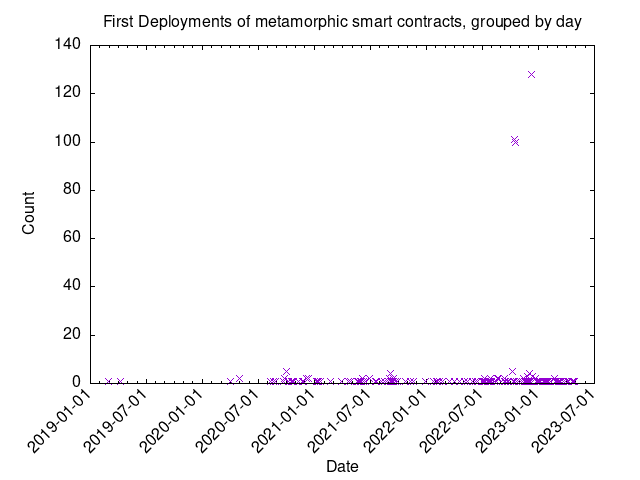
\includegraphics[width=0.9\textwidth]{Figures/analysis/metamorphic-first_deploys_outliers.png}
    \caption{First deployments of the metamorphic smart contracts.}
    \label{fig:meta-deploys-1}
\end{figure}

\begin{figure}
    \centering
    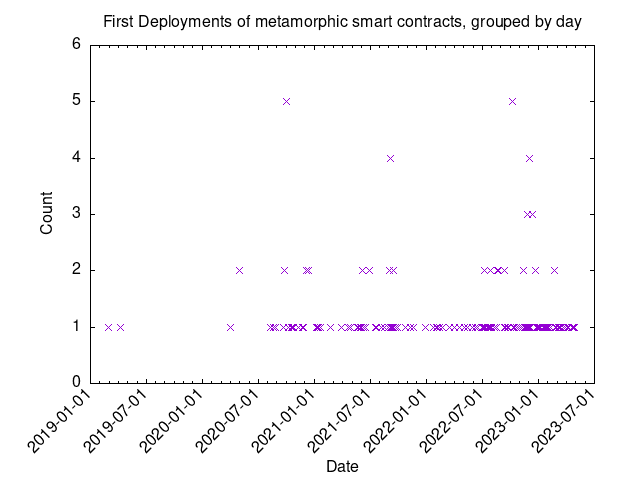
\includegraphics[width=0.9\textwidth]{Figures/analysis/metamorphic-first_deploys_no_outliers.png}
    \caption{First deployments of the metamorphic smart contracts without the three outliers.}
    \label{fig:meta-deploys-2}
\end{figure}

\begin{figure}
    \centering
    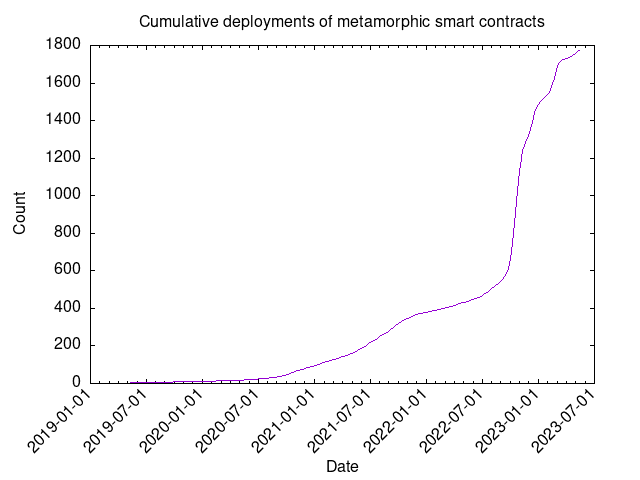
\includegraphics[width=0.9\textwidth]{Figures/analysis/metamorphic-all_deployments.png}
    \caption{Cumulative sum of all the metamorphic deployments.}
    \label{fig:meta-deploys-all}
\end{figure}

\Cref{fig:meta-deploys-1,fig:meta-deploys-2} show the first appearance of metamorphic contracts over time.
\Cref{fig:meta-deploys-1} shows all the data, while \cref{fig:meta-deploys-2} filter out three outliers. These three outliers are three days in which there were more than 100 first appearances of metamorphic smart contracts. These contracts are clearly correlated with each other. 

The cause these outliers were just two addresses\footnote{{\tt 0x3c3e8ab1e3327f24c917cd28789c9464adcf8198} and \\{\tt 0x6b25909c6141daf60ddf7c0700cedce07a9493d7} with respectively 596 and 256 metamorphic deployments.} that performed 852 deployments to metamorphic smart contracts in just three days. One of the addresses is used for MEV\footnote{MEV refers to multiple practices to maximize the extractable value from the block. It includes frontrunning, arbitrage and liquidations.} activity, while the other deployed metamorphic contracts that were all used to mint the XEN\footnote{XEN is an ERC-20 token available at \url{https://etherscan.io/token/0x06450dEe7FD2Fb8E39061434BAbCFC05599a6Fb8}} token.

\Cref{fig:meta-deploys-all} reports the cumulative sum of deployments to the 524 metamorphic smart contracts. In general, the usage of the metamorphic pattern has increased in the last period, especially since 2022.

As found by Fröwis and Böhme, many metamorphic contracts use \textit{vanity addresses}. These addresses have the peculiarity of having at least 7 leading zeros, meaning that they are smaller than the typical 20 bytes addresses. They are used to save on gas fees since it is less data that has to be stored on the blockchain. Out of the 524 metamorphic smart contracts found, 74 have a vanity address.

Understanding the purpose of metamorphic smart contracts is not easy. All the deployments do not have verified source code. Most of them have low-level bytecode with no decompiled functions (1660 out of 1781 deployments). 

I manually analyzed the top 110 metamorphic contracts by number of transactions received. I tried to understand their usage and I was able to flag the type of 98 contracts. 12 contracts were unclear what they were used for. Out of the 98 flagged contracts, 93 (94.89\%) contracts were found to be associated with MEV activity. This means that they were flagged as MEV by Etherscan or by Eigenphi\footnote{Eigenphi is a platform that collects and analyse blockchain data related to MEV activity. It is available at \url{https://eigenphi.io/}.}. The remaining 5 contracts were all used to mint the XEN token. 

This confirms the trend observed by Fröwis and Böhme, the metamorphic smart contracts are still restricted and used by a small number of users. Most of the metamorphic contracts that are effectively used for, or related to MEV activity. In many cases, the usage of this pattern is probably done for reusing vanity addresses, since they are hard to find and can have an impact on the MEV revenues.

\subsection{Similarity between metamorphic deployments}

To understand how much the code changes in between deployments of metamorphic contracts, I computed the cosine similarity between sequential deployments. For example, if a contract has received 3 deployments, I computed the similarity between the first and the second bytecodes and then between the second and the third bytecodes. The calculation of the similarity has been done as described in \cref{similarity-calculation}.

\begin{figure}
    \centering
    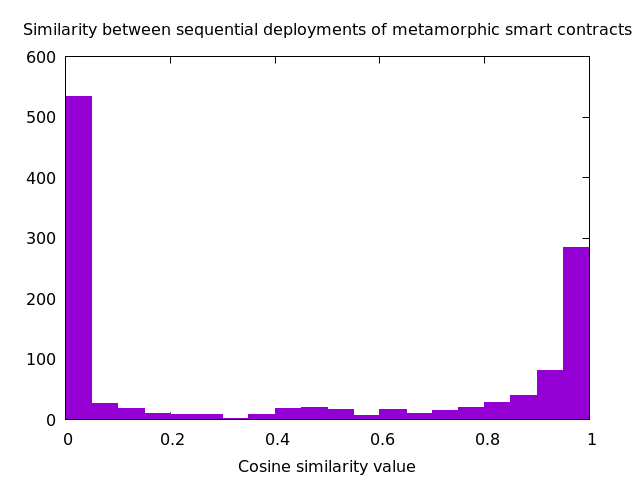
\includegraphics[width=0.9\textwidth]{Figures/analysis/metamorphic-similarities.png}
    \caption{Similarity values of all metamorphic deployments.}
    \label{fig:metamorphic-similarities}
\end{figure}
\begin{figure}
    \centering
    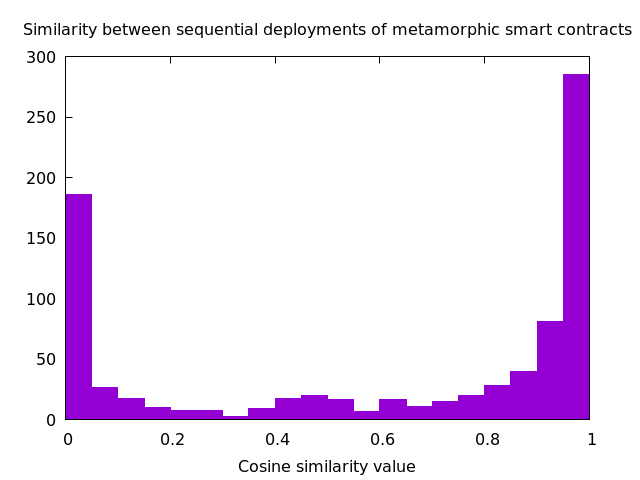
\includegraphics[width=0.9\textwidth]{Figures/analysis/metamorphic-similarities-no-pattern.png}
    \caption{Similarity values of metamorphic deployments excluding a pattern that occurred identically multiple times.}
    \label{fig:metamorphic-similarities-no-pattern}
\end{figure}

The resulting values are plotted in~\cref{fig:metamorphic-similarities}. A considerable amount of deployments completely changed the bytecode, with a similarity value of zero. Inspecting these bytecodes, I observed that most of these deployments were identical and followed a single pattern: 

\begin{itemize}
    \item The first and the second deployments were empty bytecodes.
    \item The third deployment was an implementation of the ERC-1167 minimal proxy contract.
\end{itemize}

All of the deployments that followed this pattern were done by the same address and were used to mint XEN tokens.

Excluding these deployments from the visualization showed that in the majority of cases the new bytecode is very similar to the one that is replaced. It is visible in~\cref{fig:metamorphic-similarities-no-pattern}.


\newpage

\section{Gas tokens}
\label{gas-tokens}

The aim of this analysis is to study the impact of the \textit{GasToken} pattern on Ethereum.

GasToken is a pattern that was heavily used on the Ethereum blockchain to save on gas fees. It exploited the concept of refund provided by the opcodes {\tt SELFDESTRUCT} and {\tt SSTORE}. 
I analyze and focus on the pattern that uses {\tt SELFDESTRUCT}. It works by creating and destroying basic smart contracts, used as gas reserves. 

This pattern caused the creation of many fuzzy contracts and state slots that increased the size of the Ethereum state. It was the main reason for the adoption of EIP-3529~\cite{eip-3529} on August 5th 2021. This EIP removed refunds for {\tt SELFDESTRUCT} and reduced {\tt SSTORE} refunds, effectively killing gas tokens. 

The following information explains how this pattern worked before EIP-3529. These two concepts are the fundamentals of this pattern: 

\begin{itemize}
    \item When a contract is deployed, the creator needs to pay $32000$ gas + $200$ gas for each non-zero byte stored.

    \item When a contract is destroyed, a refund of $24000$ gas is provided to the destroyer, after paying $700$ + $5000$ gas for calling {\tt CALL} + {\tt SELFDESTRUCT}. 
\end{itemize}

So the idea is that users deploy fuzzy contracts when gas is cheap and destroy them when gas is expensive. Gas from the refunds can cover up to 50\% of the gas used by the calling transaction that triggered the destructions, this is a limit introduced by the Ethereum protocol. 

To make this concept accessible, there are a few smart contracts that abstract the logic into simple tokens. For each token minted, there are many underlying smart contracts deployed. This token can easily be transferred between users. When the token is freed, the underlying smart contracts are destroyed and the owner of the token gets a discount on the gas of the transaction. The two most used tokens are CHI\footnote{Chi Gastoken on Etherscan: \url{https://etherscan.io/token/0x0000000000004946c0e9F43F4Dee607b0eF1fA1c}} and GST2\footnote{GST2 token on Etherscan: \url{https://etherscan.io/token/0x0000000000b3F879cb30FE243b4Dfee438691c04}}.

To be profitable, the price of the gas when tokens are bought must be at least half of the price of the gas when they are sold. 

Gas price has been historically very volatile, so the existence of this pattern makes sense.
\Cref{fig:gas-price} shows the historical fluctuation of gas prices.

\begin{figure}[!ht]
    \centering
    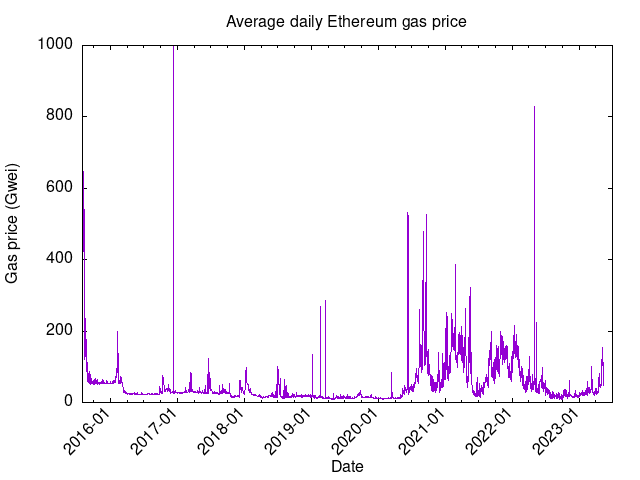
\includegraphics[width=0.9\textwidth]{Figures/analysis/gas-price.png}
    \caption{Average daily Ethereum gas price over time.}
    \label{fig:gas-price}
\end{figure}

\subsection{Identification of gas reserves}

I identified all the smart contracts ever deployed that were used as gas reserves. The logic of a gas reserve contract is basic. It simply allows one hard-coded address to destruct the contract. 
\Cref{lst:gas-token-code} shows the code that implements this logic, it is translated to the EVM bytecode reported in \cref{lst:gas-token-bytecode}

\begin{lstlisting}[caption={Pseudo code of the gas reserves.},label={lst:gas-token-code},captionpos=b,numbers=none]
if (msg.sender == GAS_TOKEN_ADDRESS) {
    SELFDESTRUCT(msg.sender);
}
\end{lstlisting}

\begin{lstlisting}[caption={EVM bytecode of the gas reserves.},label={lst:gas-token-bytecode},captionpos=b,numbers=none]
PUSH* <address of token contract>
CALLER
XOR
PC
JUMPI
CALLER
SELFDESTRUCT
\end{lstlisting}

The {\tt PUSH} opcode is represented as "{\tt *}" because there are different implementations of the gas reserve contract. Here it is possible to perform optimisations. The shortest the allowed address is and the fewer bytes are needed to be stored in the contract bytecode. This results in cheaper deployments and more efficiency of the pattern.

For example, the GST2 gastoken has this address: \\{\tt 0xb3f879cb30fe243b4dfee438691c04} that has just 15 bytes instead of the standard 20. The CHI gas token, a more recent and optimized alternative, uses\\ {\tt 0x4946c0e9f43f4dee607b0ef1fa1c} that is one less byte. Finding these short addresses is a very resource-intensive computation and requires trillions of iterations and hashes.

I identified all the gas reserves using the skeletons. There are five distinct skeletons that were used as gas reserves, with the only difference in the type of {\tt PUSH}. Some of the gas reserves were deployed multiple times at the same address. The data found is reported in \cref{table:gas-reserve-deployments}.

\begin{table}[H]
\centering
    \begin{threeparttable}
    \begin{tabular}{ c c c c } 
    \toprule
    \textbf{Skeleton} & \textbf{PUSH} & \textbf{Deployments} & \textbf{Distinct addresses} \\
    \midrule  
    \small{6d00...003318585733ff} & 14 & 12,216,500 & 12,188,707 \\ [1.2ex]
    \small{6e00...003318585733ff} & 15 & 6,809,029 & 6,765,219 \\ [1.2ex]
    \small{6f00...003318585733ff} & 16 & 568,116 & 525,202 \\ [1.2ex]
    \small{7000...003318585733ff} & 17 & 9,577 & 9,577 \\ [1.2ex]
    \small{7300...003318585733ff} & 20 & 2,138,608 & 2,138,608 \\ [1.2ex]
    \bottomrule
    \end{tabular}
    \end{threeparttable}
    \caption{Gas reserves found on Ethereum.}
    \label{table:gas-reserve-deployments}
\end{table}

A total of 21,741,830 successful gas reserve deployments were found, more than one third of all the deployments of Ethereum. 90.1\% of them have been destroyed, the remaining contracts are still alive. Users should pay gas to destroy them but without a reward is very unlikely that this will ever happen. There are 2,158,422 contracts that can potentially be stuck there forever since there is no incentive to remove them from the blockchain. The timeline of deployments and destructions is shown in \cref{fig:gastokens-timeline}. It is clearly visible how the London upgrade successfully killed this pattern.

\begin{figure}[!ht]
    \centering
    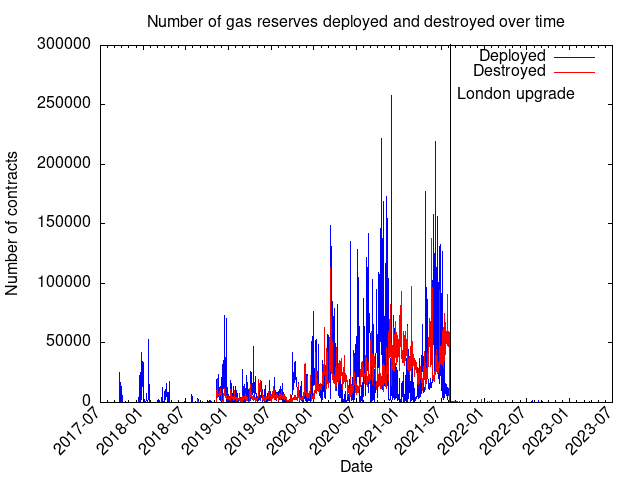
\includegraphics[width=0.9\textwidth]{Figures/analysis/gastokens-timeline.png}
    \caption{Deployments and destructions of gas reserves over time.}
    \label{fig:gastokens-timeline}
\end{figure}

\subsection{Quantification of eth saved}

I estimated the amount of Eth saved using the GasToken pattern. The calculation is performed on each gas reserve as:

\[eth_{saved}=eth_{refund}-eth_{mint}\]

\noindent where $eth_{refund}$ and $eth_{mint}$ are calculated as

\[eth_{refund} = gas_{refunded}*gas\_price_{refund\_ time}\]
\[eth_{mint}=gas_{mint}*gas\_price_{mint\_tine}\]

This is calculated on each gas reserve that was successfully deployed and then destroyed. This calculation is meant to give an order of magnitude of the amount saved.

These are the limitations and assumptions made for this calculation:

\begin{itemize}

    \item The gas spent for the small logic introduced by the token contracts that manage most of the gas reserves is not considered.
    
    \item Gas spent for the transactions that deployed the reserves is not considered. It highly depends on how many deployments were done in a single transaction. For example, doing 100 deployments in a single transaction (equivalent to minting 1 GST2 token) makes the gas of the transaction count for just 0.58\% of the deployment cost. I assume that all deployments were done in batches greater than 100 so the transaction cost is negligible.

    \item I assumed that all the destructions were done in such a way to not cover more than 50\% of the transaction gas with the refunds. Not doing so would mean wasting the refunded gas. 

    \item The gas prices used are the ones related to the blocks, obtained as the averages of the prices of gas in all the transactions. It is possible that many reserves were deployed by the miner themselves without paying for the gas.
    
\end{itemize}

The obtained value estimated a total saving of around 14K Eth, corresponding to 22,930,740 USD. The code used for this estimation is reported in \cref{lst:gas-calc}.

\begin{lstlisting}[language=Python,label={lst:gas-calc},caption={Code for computing the total Eth saved with the GasToken pattern.},captionpos=b]
# df contains all the gas reserves deployments 

# Type specifies wich PUSH was used (14, 15, ...)
# 24_000 is the refund
# 5_700 is the gas price for triggering SELFDESTRUCT + CALL
gas_refunded = 24_000 - 5_700 

# 32_000 is the cost of CREATE
# 200 is the cost for each byte stored
df['deploy_gas_used'] = 32_000 + 200 * ( 7 + df["type"] )
df['deploy_cost'] = df['deploy_price'] * df['deploy_gas_used']
df['destroy_reward'] = gas_refunded * df["destroy_price"]
df['profit'] = df['destroy_reward'] - df['deploy_cost']
saved = df['profit'].sum()
\end{lstlisting}

\newpage

\section{Most deployed functions and events}

Understanding what are the most commonly used functions and events gives a hint about what most smart contracts are doing.

I present in~\cref{table:top-functions,table:top-events} the most frequently deployed functions and events extracted using the Heimdall EVM decompiler. As explained in \cref{decompilation-section,cachine-section} the decompilation is performed on the deployed bytecode of the smart contracts, with a caching logic based on EVM skeletons. This means that two contracts sharing the same EVM skeleton received just one decompilation and the linked functions and events are the same. The numbers of this analysis depend directly on the accuracy of the decompiler.

\begin{table}[H]
\centering
    \begin{threeparttable}
    \begin{tabular}{ c c c } 
    \toprule
    \textbf{Function} & \textbf{Skeletons} & \textbf{Deployments}  \\
    \midrule
       \small{\tt sweep(address,uint256) -> bool} & 96 & 2,794,735\\ [1.2ex]
       \small{\tt flush()} & 182 & 2,775,935 \\ [1.2ex]
       \small{\tt flushTokens(address)} & 106 & 2,762,395 \\ [1.2ex]
       \small{\tt owner() -> address} & 57,643 & 2,226,240 \\ [1.2ex]
       \small{\tt tokenFallback(address,uint256,bytes)} & 68 & 1,897,675 \\ [1.2ex]
       \small{\tt implementation() -> address} & 1,472 & 1,688,820 \\ [1.2ex]
       \small{\tt proxyType() -> uint256} & 96 & 1,581,439 \\ [1.2ex]
       \small{\tt upgradeTo(address)} & 1,102 & 1,577,083 \\ [1.2ex]
       \small{\tt transferProxyOwnership(address)} & 177 & 1,556,545 \\ [1.2ex]
       \small{\tt proxyOwner() -> address} & 185 & 1,556,297 \\ [1.2ex]
       \small{\tt upgradeabilityOwner() -> address} & 127 & 1,554,012 \\ [1.2ex]
       \small{\tt upgradeToAndCall(address,bytes)} & 8 & 1,550,005 \\ [1.2ex]
       \small{\tt transferOwnership(address)} & 46,597 & 581,149 \\ [1.2ex]
       \small{\tt balanceOf(address) -> uint256} & 57,144 & 563,664 \\ [1.2ex]
       \small{\tt name() -> bytes memory} & 55,842 & 535,428 \\ [1.2ex]
       \small{\tt symbol() -> bytes memory} & 54,714 & 530,246 \\ [1.2ex]
       \small{\tt totalSupply() -> uint256} & 54,511 & 529,351 \\ [1.2ex]
       \small{\tt transfer(address,uint256)} & 46,024 & 526,022 \\ [1.2ex]
       \small{\tt approve(address,uint256) -> uint256} & 51,984 & 515,168 \\ [1.2ex]
       \small{\tt decimals() -> bool} & 44,682 & 503,589 \\ [1.2ex]
    \bottomrule
    \end{tabular}
    \end{threeparttable}
    \caption{Top 20 functions by number of deployments.}
    \label{table:top-functions}
\end{table}

\begin{table}[H]
\centering
    \begin{threeparttable}
    \begin{tabular}{ c c c } 
    \toprule
    \textbf{Event} & \textbf{Skeletons} & \textbf{Deployments}  \\
    \midrule
       \small{\tt TokensFlushed(address,uint256)} & 14 & 2,720,369\\ [1.2ex]
       \small{\tt Upgraded(address)} & 1,115 & 1,577,868\\ [1.2ex]
       \small{\tt ProxyOwnershipTransferred(address,address)} & 165 & 1,556,455\\ [1.2ex]
       \small{\tt OwnershipTransferred(address,address)} & 41,985 & 516,317\\ [1.2ex]
       \small{\tt Transfer(address,address,uint256)} & 47,380 & 494,780 \\ [1.2ex]
       \small{\tt Approval(address,address,uint256)} & 48,499 & 482,358 \\ [1.2ex]
       \small{\tt OwnerChanged(address)} & 133 & 430,676 \\ [1.2ex]
       \small{\tt DeedClosed()} & 4 & 430,173 \\ [1.2ex]
       \small{\tt SafeModeActivated(address)} & 51 & 231,379 \\ [1.2ex]
       \small{\tt TokenTransfer(address,address,uint256)} & 11 & 84,781 \\ [1.2ex]
       \small{\tt Transfer(address,uint256)} & 64 & 63,185 \\ [1.2ex]
       \small{\tt TokenReleased(address,uint256)} & 14 & 49,736 \\ [1.2ex]
       \small{\tt Burn(address,uint256)} & 3,136 & 37,404 \\ [1.2ex]
       \small{\tt OwnershipRenounced(address)} & 2,408 & 24,993 \\ [1.2ex]
       \small{\tt ApprovalForAll(address,address,bool)} & 10,063 & 22,451 \\ [1.2ex]
       \small{\tt AdminChanged(address,address)} & 520 & 20,353 \\ [1.2ex]
       \small{\tt LogSetOwner(address)} & 196 & 16,921 \\ [1.2ex]
       \small{\tt DelegateUpgraded(address,address,uint256)} & 2 & 14,076 \\ [1.2ex]
       \small{\tt DelegateRolledBack(address,address,uint256)} & 2 & 14,076 \\ [1.2ex]
    \bottomrule
    \end{tabular}
    \end{threeparttable}
    \caption{Top 20 events by number of deployments.}
    \label{table:top-events}
\end{table}

All the functions are related to proxy, wallet, or token contracts. For the events, it is the same situation. There is the event {\tt DeedClosed} that is related to ENS\footnote{ENS (Ethereum Name Service) is a decentralized name service \url{https://ens.domains/}.} and  {\tt DelegateUpgraded} and {\tt DelegateRolledBack} that are used for the Rocket Pool\footnote{Rocket Pool is a decentralized staking pool \url{https://rocketpool.net/}.} protocol, but both of these protocols are token-based.

\newpage

\section{Contracts metadata}

Smart contracts deployed using the Solidity compiler have the default option to include CBOR-encoded data at the end of the deployed bytecode. This piece of information includes:

\begin{itemize}
    \item The hash of the contract metadata. The metadata includes any kind of information related to the smart contract, such as the ABI, the documentation, the settings of the compiler, etc. It also includes the hash of the source code, so a change in the source code causes a change in the metadata that consequently changes its hash. This hash can be used as an address to store and retrieve the actual metadata and source code of the contract on a decentralized file system.
    \item The type of the hash ({\tt bzzr0}, {\tt bzzr1} or {\tt IPFS}).
    \item A flag stating if the compilation was done with experimental features of the compiler enabled.
    \item The version of the Solidity compiler used.
\end{itemize}

All of this data has been extracted by eth2dgraph with a regex as explained in \cref{skeleton-section}. Here is an overview of what has been extracted.

\subsection{Hash of metadata}

A total 17,491,909 deployments included the hash of the metadata in the bytecode stored on the blockchain. Out of these, 1,164,973 (6.66\%) used {\tt IPFS}, 15,636,747 (89.39\%) used {\tt bzzr0} and 690,189 (3.94\%) used {\tt bzzr1}. 

Analyzing the values of the hashes, there were just 770,719 distinct hashes found. This means that, on average, each smart contract compiled with the Solidity compiler gets deployed 22.7 times, another indicator of the high code reuse in the Ethereum blockchain. There are five occurrences in which the same metadata hash has been deployed more than 1M times, all of these deployments were done by just a few distinct addresses. On the other hand, there are 690,157 occurrences in which the hash was only used once.

\subsection{Experimental compilations}

The Solidity compiler allows to activate experimental features that are not already included by default in the decompiler. This can be done at the beginning of the code writing {\tt pragma experimental <feature-name>}. Inside the CBOR encoded data appended at the end of the generated bytecode there is a boolean stating whether any experimental feature was used or not.

Out of the 17,491,909 deployments that included the CBOR encoded data, 1,113,139 (6.36\%) had experimental features activated. These contracts with experimental features received a total of 5.8M transactions.

\subsection{Solc versions}

2,090,487 smart contracts included the version of the Solidity compiler in the CBOR-encoded data. The version is included just from Solidity v0.5.9 onward. There are 1,299 smart contracts that included fake Solidity versions (e.g. 100.67.137, 116.153.33, etc.) and were removed in this analysis. 32 deployments were found to use pre-releases of the compiler, in these cases Solidity appends the exact commit used. The total numbers of major versions found are reported in~\cref{table:solc-majors}.

\begin{table}[ht]
\centering
    \begin{threeparttable}
    \begin{tabular}{ c c } 
    \toprule
    \textbf{Major Solidity version} & \textbf{Number of deployments} \\
    \midrule
       0.5 & 925,506 \\ [1.2ex]
       0.6 & 287,552 \\ [1.2ex]
       0.7 & 215,924 \\ [1.2ex]
       0.8 & 660,206 \\ [1.2ex]
    \bottomrule
    \end{tabular}
    \end{threeparttable}
    \caption{Numbers of deployments found per major version of the Solidity compiler.}
    \label{table:solc-majors}
\end{table}

\Cref{fig:deploys-per-solidity-version} shows the distribution over time of the various major Solidity versions found. 
Generally, it is possible to observe how old compiler versions remain heavily used even after the release of multiple new versions.
The versions 0.6 and 0.7 almost never managed to have a higher amount of daily deployments than the 0.5 version.
The latest version, 0.8, managed to overtake the 0.5 after around one year since its release. Now it is the most used Solidity version.

\begin{figure}[ht]
    \centering
    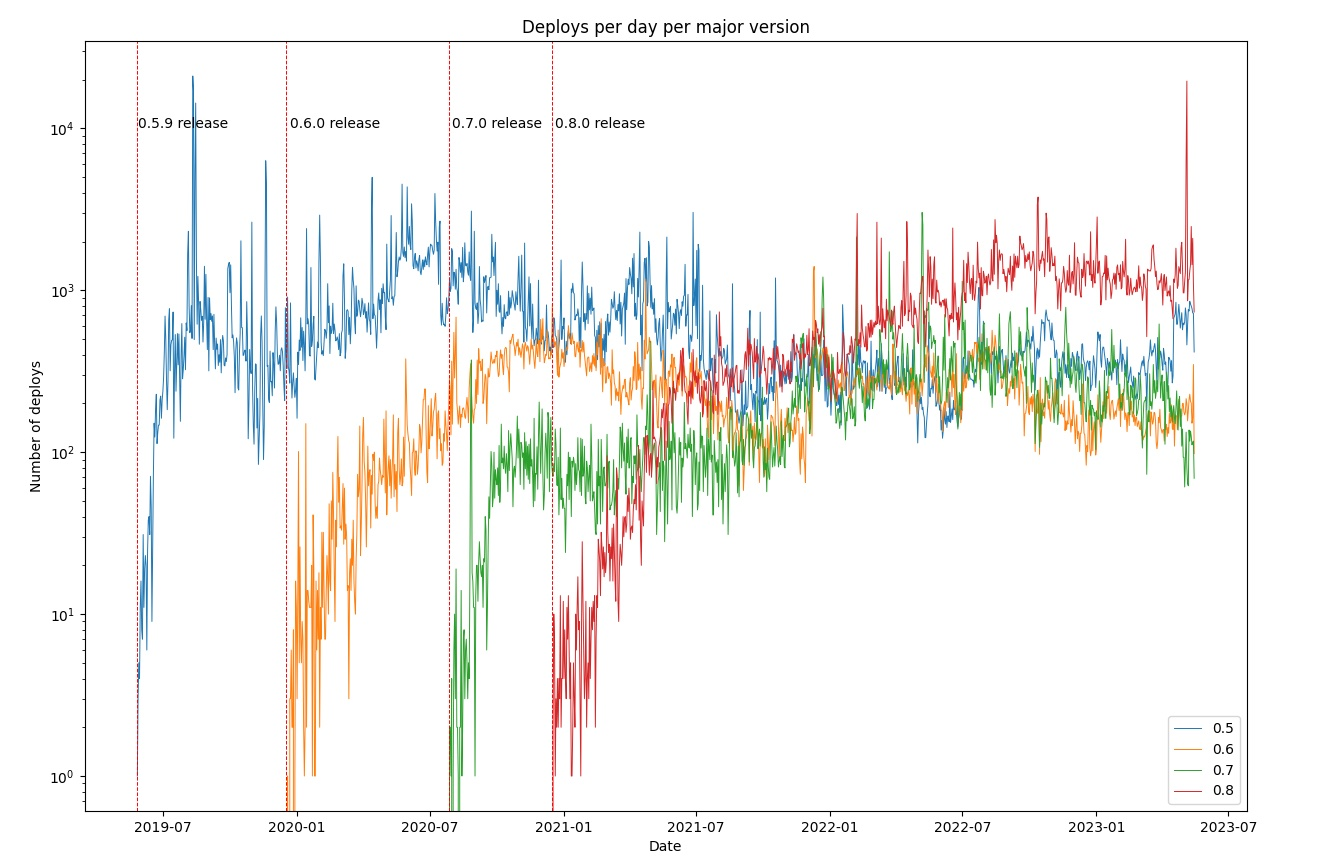
\includegraphics[width=0.95\textwidth]{Figures/analysis/deploys_per_day_per_major.jpg}
    \caption{Deployments over time divided by major Solidity compiler versions. Each data entry represents the daily amount of deployments found per version. Keep in mind the log scale.}
    \label{fig:deploys-per-solidity-version}
\end{figure}





\cleardoublepage

\chapter{Discussion}
\label{chapter-discussion}

\subsection{Dgraph for Ethereum data}

As blockchain technology gains popularity, the challenge of managing data from these networks becomes increasingly critical. Dgraph proved to be a viable solution for managing Ethereum data. This kind of data adapts well to graph databases. 

However, there are some drawbacks that were encountered when using Dgraph:

\begin{itemize}
    \item EVM data is often represented using 256-bit integers or raw bytes. Dgraph does not support these data types. They must be stored as text with all the related disadvantages, such as more disk space used and the impossibility of doing math operations in the queries.
    \item When used with a large dataset, Dgraph encountered some limitations with the usage of memory. It crashed both during the bulk import and during the execution of large queries. These problems were solved by modifying the database source code or tweaking the queries to use less memory. However, they show that Dgraph is still not well-tested against large datasets.
    \item Insertion of live Ethereum data into a cluster with all the history of the blockchain was slower that the production of data from the blockchain. The underlying Badger database gets stuck periodically logging~{\tt L0 was stalled}. This made it impossible to keep the dataset updated with the latest blocks. 
\end{itemize}

Dgraph is a relatively new technology. It was born in 2016 and is currently under active development. The project maintainers showed interest in this use case and actively helped me to solve the problems I faced with the database.

\subsection{Challenges of blockchain data management}

The process of data extraction using the Ethereum RPC interface worked well and proved to be an optimal solution. The biggest problem of this process is the amount of time and computational resources it needs, as described in \Cref{chapter-5}.

It is important to highlight that these data refer to the Ethereum blockchain. Layer 2 protocols and other blockchains are even more critical as they are already producing more data than Ethereum. Polygon\footnote{Polygon is a layer 2 EVM blockchain based on Ethereum.} is producing blocks 6 times faster than Ethereum, with an average of one new block every two seconds. The BNB Chain\footnote{BNB Chain is a layer 1 EVM compatible blockchain developed by the Binance exchange.} is another popular blockchain that is growing at a pace of a new block every three seconds.

Another relevant concern is that blockchains will grow indefinitely. The size of an instance of a Geth archive node is growing at around 3.5TB per year\footnote{This graph made by Etherscan shows the historical size of a Geth archive node: \url{https://etherscan.io/chartsync/chainarchive}.}. Soon, it will not be possible to handle all this data on a single machine, since vertical scalability is not infinite. A distributed approach will be the only viable way in the future.

This expensive entry barrier makes it hard to perform such an operation. People interested in analyzing Ethereum data are more likely to use one of the few centralized services instead of running their infrastructure. 

The lack of research and tools in this field could potentially create a gap between companies and the open-source community. This would reduce the decentralization of the blockchain ecosystem, making an important element such as data analysis dependent on private companies.

\subsection{Domain-specific data analysis}

If blockchains continue to grow in size indefinitely as they are designed to do, it will be unfeasible to get and index all the historical data in a single place. Chances are that it will be a similar challenge of indexing all the history of the World Wide Web on a single machine or cluster of machines right now.

The potential solution to this problem is reducing the domain of the managed data. As seen in the analysis reported in \Cref{chapter-analysis}, most of the traffic on the chain is restricted to a relatively small set of smart contracts. These smart contracts implement different and independent protocols. Information about what happens in these protocols can be extracted, indexed and analyzed independently from each other.

The Graph~\cite{the-graph} proposes a solution of this kind. As noted in \Cref{chapter-3}, this decentralized indexing protocol gathers together data that is indexed independently from the various decentralized protocols implemented by smart contracts. This particular indexing protocol is even more strict in term of amount of data since it just considers the logs, ignoring transactions and blocks data. This technique allows for better scalability, but lacks giving a bigger picture of the traffic in a blockchain network.

\subsection{Future work}

There are some areas of this research that could be explored more in-depth in future works. In theory, eth2dgraph should work with any EVM-compatible chain, such as Polygon, since the RPCs used are the same. This has not been tested because of the lack of available nodes.

Due to the infrastructure available, Dgraph was used in a single machine. It would be interesting to test its behaviour with a cluster distributed over multiple servers. This would test the horizontal scalability of Dgraph.

Another area of improvement is the streaming of live data. Currently, eth2dgraph supports live data insertion from the Ethereum network to an active Dgraph cluster using ACID transactions. It proved to work well when the database does not have a lot of data already indexed, but it was slower than the production of data from the blockchain when the database had all the Ethereum history indexed. The optimization of this part of the tool was not the priority of this work, so this could be an area of improvement.

Talking more broadly, the optimal solution to the problem that this research tries to address would be to have blockchain clients that directly give the option to freely index data. This would remove the redundancy of having to store data in two different places: one in the EVM client storage and one in the database storage. These \textit{Blockchain Analytics Clients} could specifically target data analysts and would not need the ability to participate in the consensus layer of the protocol. 



\cleardoublepage

\chapter{Conclusions}
\label{chapter-conclusions}

This research has investigated a novel solution to the problem of Ethereum data management using a graph database. Thanks to the release of eth2dgraph, it is now possible to easily index Ethereum data using Dgraph and query it with DQL and GraphQL. 

To answer research question 1, the schema used to manage data gives a clear image of what can be extracted from EVM blockchains without relying on centralized services. It is reported in \cref{fig:schema}. The only kind of information that can not be extracted without relying on centralized services is the source code of smart contracts. It is possible to extract functions and events implemented by smart contracts from their bytecodes, even if the data is not perfectly accurate.

Generally, most of the semantics related to on-chain operations can be obtained from logs. In this work, logs referring to token transfers were parsed to allow faster and easier queries. The same can be done for other domains, e.g. token swaps, token approvals, or other protocol-specific use cases.

To answer the second research question, with the solution provided in this Master's Thesis, it is possible to estimate that at least 6TB of fast SSDs, 400GB of RAM, and a CPU of 64 cores are needed to perform independent extraction and indexing of all Ethereum data as of August 2023. 

Although the entry barrier is high, it is still possible to run an archive node, extract all the historical data, and index it in a database all in the same machine. Apart from computational resources, it is an operation that also takes time. It takes at least a few days to sync a node, around seven hours to extract the data and more than two days to ingest it into the database.

The analysis on the extracted data conducted in \Cref{chapter-analysis} serve as an example of the potentiality of this data. They show possible ways of using and interpreting Ethereum data. From these analysis it appeared that most of the traffic on the network is restricted to a small number of smart contracts. This fact suggested that more efficient analysis can be done focusing on a specific decentralized protocol, instead of having to manage all the historical Ethereum data.


\cleardoublepage


\addcontentsline{toc}{chapter}{\protect\numberline{}References}
\printbibliography[title={References}] %you may change the title in the toc here if you want
\cleardoublepage



\chapter*{\LARGE \textbf{Appendices}}
\fancyhf{} %clear the header, it should be empty for the appendices
\renewcommand{\headrulewidth}{0pt} %no rule
\fancyfoot[C]{\thepage} %set the page numbers in the center of the footer instead 

%it is possible to set a different page numbering style for the appendix, but I personally just continued with the same page numbering as the main content as I find that more tidy
%\pagenumbering{roman}
%\setcounter{page}{1}
\addcontentsline{toc}{chapter}{\protect\numberline{}Appendices:}
\appendix

\chapter*{A - Complete schema of indexed data}
{\label[appendix]{app-b}}
\addcontentsline{toc}{chapter}{\protect\numberline{}B - Complete schema of indexed data} 

Here are both the DQL and GraphQL schema of the data extracted.
\cref{lst:dql-schema} reports the DQL schema and \cref{lst:graphql-schema} the GraphQL one.

\begin{lstlisting}[
caption={DQL schema of indexed data},
label={lst:dql-schema}
]
<Account.address>: string @index(hash) @upsert .
<Account.tags>: [string] @index(hash) .
<Account.is_contract>: bool @index(bool) .
<Block.base_fee_per_gas>: float .
<Block.datetime>: datetime @index(hour) .
<Block.difficulty>: string @index(hash) .
<Block.gas_limit>: int .
<Block.gas_used>: int @index(int) .
<Block.gas_price_avg>: float @index(float) .
<Block.gas_price_max>: float .
<Block.gas_price_min>: float .
<Block.gas_price_std_dev>: float .
<Block.number>: int @index(int) @upsert .
<Block.size>: int .
<Block.tx_count>: int .
<Block.miner>: uid @reverse .
<Block.withdrawals>: [uid] @reverse .
<ContractDeployment.block>: uid @reverse .
<ContractDeployment.contract>: uid @reverse .
<ContractDeployment.creation_bytecode>: string .
<ContractDeployment.creator>: uid @reverse .
<ContractDeployment.deployed_bytecode>: string .
<ContractDeployment.experimental>: bool .
<ContractDeployment.failed_deploy>: bool .
<ContractDeployment.skeleton>: uid @reverse .
<ContractDeployment.solc_version>: string .
<ContractDeployment.storage_address>: string .
<ContractDeployment.storage_protocol>: string .
<ContractDeployment.tx_hash>: string @index(hash) .
<ContractDeployment.name>: string @index(trigram) .
<ContractDeployment.verified_source>: bool @index(bool) .
<ContractDeployment.verified_source_code>: string @index(term) .
<ContractDestruction.balance_left>: string .
<ContractDestruction.block>: uid @reverse .
<ContractDestruction.contract>: uid @reverse .
<ContractDestruction.refound_address>: uid .
<ContractDestruction.failed>: bool @index(bool) .
<ContractDestruction.tx_hash>: string @index(hash) .
<Error.inputs>: string @index(trigram) .
<Error.name>: string @index(exact) .
<Error.signature>: string @index(hash) @upsert .
<Event.inputs>: string @index(trigram) .
<Event.name>: string @index(exact) .
<Event.signature>: string @index(hash) @upsert .
<Function.inputs>: string @index(trigram) .
<Function.name>: string @index(exact) .
<Function.bytes4>: string @index(hash) .
<Function.outputs>: string @index(trigram) .
<Function.signature>: string @index(hash) @upsert .
<Skeleton.bytecode>: string @index(hash) .
<Skeleton.erc20_compliancy>: int @index(int) .
<Skeleton.erc721_compliancy>: int @index(int) .
<Skeleton.errors>: [uid] @reverse .
<Skeleton.events>: [uid] @reverse .
<Skeleton.failed_decompilation>: bool .
<Skeleton.functions>: [uid] @reverse .
<Skeleton.similar_code>: [uid] .
<Skeleton.similar_interface>: [uid] .
<TokenTransfer.block>: uid @reverse .
<TokenTransfer.contract>: uid @reverse .
<TokenTransfer.from>: uid @reverse .
<TokenTransfer.to>: uid @reverse .
<TokenTransfer.tx>: uid .
<TokenTransfer.value>: string .
<TokenTransfer.token_id>: string @index(hash) .
<Transaction.block>: uid @reverse .
<Transaction.from>: uid @reverse .
<Transaction.gas>: int .
<Transaction.gas_price>: int .
<Transaction.hash>: string @index(hash) @upsert .
<Transaction.input>: string .
<Transaction.bytes4>: string @index(hash) .
<Transaction.max_fee_per_gas>: int .
<Transaction.max_priority_fee_per_gas>: int .
<Transaction.nonce>: int .
<Transaction.r>: string .
<Transaction.s>: string .
<Transaction.to>: uid @reverse .
<Transaction.v>: string .
<Transaction.value>: string .
<Log.contract>: uid @reverse .
<Log.block>: uid @reverse .
<Log.tx>: uid @reverse .
<Log.topic_0>: string @index(hash) .
<Log.topic_1>: string @index(hash) .
<Log.topic_2>: string @index(hash) .
<Log.topic_3>: string @index(hash) .
<Log.data>: string .
<Log.tx_index>: int .
<Log.index>: int .
<Withdrawal.address>: uid @reverse .
<Withdrawal.string>: int .
<Withdrawal.index>: int .
<Withdrawal.validator_index>: int .
<Withdrawal.amount>: int .
type <Account> {
	Account.address
	Account.tags
	Account.is_contract
}
type <Block> {
	Block.number
	Block.datetime
	Block.difficulty
	Block.tx_count
	Block.gas_price_min
	Block.gas_price_max
	Block.gas_price_avg
	Block.gas_price_std_dev
	Block.gas_limit
	Block.gas_used
	Block.base_fee_per_gas
	Block.size
	Block.miner
	Block.withdrawals
}
type <ContractDeployment> {
	ContractDeployment.contract
	ContractDeployment.block
	ContractDeployment.creator
	ContractDeployment.tx_hash
	ContractDeployment.failed_deploy
	ContractDeployment.creation_bytecode
	ContractDeployment.deployed_bytecode
	ContractDeployment.skeleton
	ContractDeployment.storage_protocol
	ContractDeployment.storage_address
	ContractDeployment.experimental
	ContractDeployment.solc_version
	ContractDeployment.verified_source
	ContractDeployment.verified_source_code
	ContractDeployment.name
}
type <ContractDestruction> {
	ContractDestruction.contract
	ContractDestruction.block
	ContractDestruction.tx_hash
	ContractDestruction.balance_left
	ContractDestruction.refound_address
	ContractDestruction.failed
}
type <Error> {
	Error.signature
	Error.name
	Error.inputs
}
type <Event> {
	Event.signature
	Event.name
	Event.inputs
}
type <Function> {
	Function.signature
	Function.name
	Function.inputs
	Function.outputs
}
type <Skeleton> {
	Skeleton.bytecode
	Skeleton.functions
	Skeleton.events
	Skeleton.errors
	Skeleton.failed_decompilation
	Skeleton.erc20_compliancy
	Skeleton.erc721_compliancy
	Skeleton.similar_code
	Skeleton.similar_interface
}
type <TokenTransfer> {
	TokenTransfer.contract
	TokenTransfer.from
	TokenTransfer.to
	TokenTransfer.value
	TokenTransfer.block
	TokenTransfer.tx
	TokenTransfer.token_id
}
type <Transaction> {
	Transaction.hash
	Transaction.from
	Transaction.to
	Transaction.block
	Transaction.value
	Transaction.gas
	Transaction.gas_price
	Transaction.input
	Transaction.bytes4
	Transaction.max_fee_per_gas
	Transaction.max_priority_fee_per_gas
	Transaction.nonce
	Transaction.r
	Transaction.s
	Transaction.v
}
type <Log> {
	Log.contract
	Log.block
	Log.tx
	Log.topic_0
	Log.topic_1
	Log.topic_2
	Log.topic_3
	Log.data
	Log.tx_index
	Log.index
}
type <Withdrawal> {
	Withdrawal.address
	Withdrawal.amount
	Withdrawal.index
	Withdrawal.validator_index
}
\end{lstlisting}

\begin{lstlisting}[
caption={GraphQL schema of indexed data},
label={lst:graphql-schema}
]
type Account {
  address: String! @id @search(by: [hash])
  tags: [String] @search(by: [hash])
  is_contract: Boolean @search
  token_sent: [TokenTransfer] @dgraph(pred: "~TokenTransfer.from")
  token_received: [TokenTransfer] @dgraph(pred: "~TokenTransfer.to")
  transactions_sent: [Transaction] @dgraph(pred: "~Transaction.from")
  transactions_received: [Transaction] @dgraph(pred: "~Transaction.to")
  created_contracts: [ContractDeployment] @dgraph(pred: "~ContractDeployment.creator")
  logs: [Log] @dgraph(pred: "~Log.contract")
  deployments: [ContractDeployment] @dgraph(pred:"~ContractDeployment.contract")
  destructions: [ContractDestruction] @dgraph(pred:"~ContractDestruction.contract")
  transfers: [TokenTransfer] @dgraph(pred: "~TokenTransfer.contract")
  mined_blocks: [Block] @dgraph(pred:"~Block.miner")
  withdrawals: [Withdrawal] @dgraph(pred:"~Withdrawal.address")
}

type Withdrawal {
  amount: String! @search
  index: Int
  validator_index: Int
  address: Account! @dgraph(pred:"Withdrawal.address")
  block: [Block] @dgraph(pred:"~Block.withdrawals")
}

type Block {
  number: Int! @id @search
  miner: Account @dgraph(pred:"Block.miner")
  datetime: DateTime @search(by: [hour])
  difficulty: String @search
  tx_count: Int @search
  gas_price_min: Float
  gas_price_max: Float
  gas_price_avg: Float @search
  gas_price_std_dev: Float
  gas_limit: Int
  gas_used: Int
  base_fee_per_gas: Float
  size: Int
  deployments: [ContractDeployment] @dgraph(pred: "~ContractDeployment.block")
  destructions: [ContractDestruction] @dgraph(pred: "~ContractDestruction.block")
  transfers: [TokenTransfer] @dgraph(pred: "~TokenTransfer.block")
  transactions: [Transaction] @dgraph(pred: "~Transaction.block")
  withdrawals: [Withdrawal] @dgraph(pred:"Block.withdrawals")
  logs: [Log] @dgraph(pred: "~Log.block")
}

type Transaction {
  hash: String! @id @search(by: [hash])
  value: String! 
  gas: Int @search
  gas_price: Int @search
  input: String
  bytes4: String @search(by: [hash])
  max_fee_per_gas: Int
  max_priority_fee_per_gas: Int
  nonce: Int
  r: String
  s: String
  v: String
  from: Account! @dgraph(pred:"Transaction.from")
  to: Account! @dgraph(pred:"Transaction.to")
  block: Block! @dgraph(pred:"Transaction.block")
  logs: [Log] @dgraph(pred: "~Log.tx")
}

type Function {
  signature: String! @id @search(by: [hash])
  name: String @search(by: [exact])
  inputs: String @search(by: [trigram])
  outputs: String @search(by: [trigram])
  skeletons: [Skeleton] @dgraph(pred:"~Skeleton.functions")
  bytes4: String @search(by: [hash])
}

type Event {
  signature: String! @id @search(by: [hash])
  name: String @search(by: [exact])
  inputs: String @search(by: [trigram])
  skeletons: [Skeleton] @dgraph(pred:"~Skeleton.events")
}

type Error {
  signature: String! @id @search(by: [hash])
  name: String @search(by: [exact])
  inputs: String @search(by: [trigram])
  skeletons: [Skeleton] @dgraph(pred:"~Skeleton.errors")
}

type ContractDeployment {
  tx_hash: String @search(by: [hash])
  failed_deploy: Boolean @search
  creation_bytecode: String
  deployed_bytecode: String
  storage_protocol: String
  storage_address: String
  experimental: Boolean @search
  solc_version: String @search(by: [hash])
  verified_source: Boolean @search
  verified_source_code: String @search(by: [term])
  name: String @search(by: [trigram])
  contract: Account! @dgraph(pred:"ContractDeployment.contract")
  block: Block! @dgraph(pred:"ContractDeployment.block")
  creator: Account! @dgraph(pred:"ContractDeployment.creator")
  skeleton: Skeleton @dgraph(pred:"ContractDeployment.skeleton")
}

type ContractDestruction {
  tx_hash: String @search(by: [hash])
  balance_left: String
  refound_address: Account! @dgraph(pred:"ContractDestruction.refound_address")
  contract: Account! @dgraph(pred:"ContractDestruction.contract")
  block: Block! @dgraph(pred:"ContractDestruction.block")
}

type Skeleton {
  bytecode: String! @search(by: [hash])
  erc20_compliancy: Int @search
  erc721_compliancy: Int @search
  failed_decompilation: Boolean @search
  deployments: [ContractDeployment] @dgraph(pred:"~ContractDeployment.skeleton")
  functions: [Function] @dgraph(pred:"Skeleton.functions")
  events: [Event] @dgraph(pred:"Skeleton.events")
  errors: [Error] @dgraph(pred:"Skeleton.errors")
  similar_code: [Skeleton]
  similar_interface: [Skeleton]
}

type TokenTransfer {
  value: String!
  token_id: String
  tx: Transaction
  block: Block! @dgraph(pred:"TokenTransfer.block")
  contract: Account! @dgraph(pred:"TokenTransfer.contract")
  from: Account! @dgraph(pred:"TokenTransfer.from")
  to: Account! @dgraph(pred:"TokenTransfer.to")
}

type Log {
  topic_0: String @search(by: [hash])
  topic_1: String @search(by: [hash])
  topic_2: String @search(by: [hash])
  topic_3: String @search(by: [hash])
  data: String 
  tx_index: Int
  index: Int
  contract: Account! @dgraph(pred:"Log.contract")
  block: Block @dgraph(pred:"Log.block")
  tx: Transaction @dgraph(pred:"Log.tx")
}
\end{lstlisting}

\chapter*{B - Data returned from Ethereum RPCs}
\addcontentsline{toc}{chapter}{\protect\numberline{}B - Data returned from RPCs} 

To give more context, \cref{lst:block-data-rpc,lst:log-data-rpc,lst:trace-data-rpc} include three examples of data returned from the RPCs that were used for extracting Ethereum data.

\subsection*{eth\_getBlockByNumber}

\begin{lstlisting}[
caption={Data returned from eth\_getBlockByNumber RPC with hydrated transactions.},
label={lst:block-data-rpc}
]
{
    "jsonrpc": "2.0",
    "id": 1,
    "result": {
        "baseFeePerGas": "0x1ced5e1e0c",
        "difficulty": "0x0",
        "extraData": "0x7273796e632d6275696c6465722e78797a",
        "gasLimit": "0x1c9c380",
        "gasUsed": "0xd0b9ef",
        "hash": "0x...",
        "logsBloom": "0x...",
        "miner": "0x1f9090aae28b8a3dceadf281b0f12828e676c326",
        "mixHash": "0x...",
        "nonce": "0x0000000000000000",
        "number": "0x1067381",
        "parentHash": "0x...",
        "receiptsRoot": "0x...",
        "sha3Uncles": "0x...",
        "size": "0x135f5",
        "stateRoot": "0x...",
        "timestamp": "0x6455fe73",
        "totalDifficulty": "0xc70d815d562d3cfa955",
        "transactions": [
            ...,
            {
                "blockHash": "0x...",
                "blockNumber": "0x1067381",
                "from": "0x...",
                "gas": "0x1725d",
                "gasPrice": "0x1cf069692b",
                "maxPriorityFeePerGas": "0x30b4b1f",
                "maxFeePerGas": "0x1df5b2c880",
                "hash": "0x...",
                "input": "0x...",
                "nonce": "0x8",
                "to": "0x...",
                "transactionIndex": "0x9b",
                "value": "0x0",
                "type": "0x2",
                "accessList": [],
                "chainId": "0x1",
                "v": "0x1",
                "r": "0x...",
                "s": "0x..."
                },
                ...
        ],
        "transactionsRoot": "0x...",
        "uncles": [],
        "withdrawals": [
            ...,
            {
                "index": "0x285032",
                "validatorIndex": "0x7125d",
                "address": "0x562ab7dca86f8947f5b066a663d83452954a71a2",
                "amount": "0xbcd8a1"
            },
            ...
        ],
        "withdrawalsRoot": "0x..."
    }
}
\end{lstlisting}

\subsection*{eth\_getLogs}

\begin{lstlisting}[
caption={Data returned from eth\_getLogs RPC.},
label={lst:log-data-rpc}
]
{
  "jsonrpc": "2.0",
  "id": 1,
  "result": [
    ...,
    {
      "address": "0xa0b86991c6218b36c1d19d4a2e9eb0ce3606eb48",
      "topics": [
        "0x...",
        "0x...",
        "0x..."
      ],
      "data": "0x...",
      "blockNumber": "0xe524e1",
      "transactionHash": "0x...",
      "transactionIndex": "0xb",
      "blockHash": "0x...",
      "logIndex": "0x0",
      "removed": false
    },
    ...
  ]
}
\end{lstlisting}

\subsection*{trace\_block}

\begin{lstlisting}[
caption={Data returned from trace\_block RPC.},
label={lst:trace-data-rpc}
]
{
  "jsonrpc": "2.0",
  "id": 1,
  "result": [
  ...,
  {
    "action": {
      "from": "0xaeec6f5aca72f3a005af1b3420ab8c8c7009bac8",
      "callType": "call",
      "gas": "0x11170",
      "input": "0x",
      "to": "0xef86d3164a50df780e24e9226bcddf3c8606e424",
      "value": "0x2b5e3af16b1880000"
    },
    "blockHash": "0x...",
    "blockNumber": 5469798,
    "result": {
      "gasUsed": "0x0",
      "output": "0x"
    },
    "subtraces": 0,
    "traceAddress": [],
    "transactionHash": "0x...",
    "transactionPosition": 0,
    "type": "call"
  },
  ...
  ]
}
\end{lstlisting}



\end{document}
